%%%%%%%%%%%%%%%%%%%%%%%%%%%%%%%%%%%%%%%%%%%%%%%%%%%%%%%%%%%%%%
%                     Gerardo Mazzei                         %
%  based on Luke Van Hulle's and Christian Schaefer's thesis %
%%%%%%%%%%%%%%%%%%%%%%%%%%%%%%%%%%%%%%%%%%%%%%%%%%%%%%%%%%%%%%

% The main thesis document

%% These arara commands are placed here to show the order of operations required to compile this document. If you want to use arara with the subfiles package then these commands will also need to go in every included file. Arara is convenient for multiple workstation compilation and when you need other people to be able to build your document but so far I am not very satisfied with the error reports it generates. Hopefully version 4.0 has a little more documentation and fixes these problems.

% arara: pdflatex
% arara: nomencl
% arara: bibtex
% arara: pdflatex
\documentclass[ 12pt, letterpaper, twoside, openany]{book}

%These files define a lot of the formatting and commands used throughout the document
% 02_Inputs.tex
% the packages are put in a seperate file to help keep the main.tex file clean

% To use the fontec package properly make sure the cm-super
% package is installed for MikTex.
% https://docs.miktex.org/2.9/manual/pkgmgt.html
\usepackage[T1]{fontenc}
\usepackage{fancyhdr}

\usepackage[textwidth=65pt]{todonotes}
\usepackage{siunitx} % provides formating for numbers with SI units

\usepackage{subfiles} % For being able to compile the subfiles on their own
\usepackage{amsmath}

\usepackage{lipsum} % Used for making dummy text

\usepackage{booktabs} % Makes tables better
\usepackage{tablefootnote} % for making footnotes in tables

% used for loading graphics
\usepackage{graphicx}
\graphicspath{{Figures/}}
% used for making sub-figures
\usepackage{subfig}
%used for placing text over images
\usepackage[percent]{overpic}

% Helps with making arrow with overpic
\usepackage{pict2e}

% use the \layout command and compile to show margins
\usepackage{layout}

% For figures with text wrapped around them
\usepackage{wrapfig}

% For special formating of lists
\usepackage{enumitem}


\usepackage{nomencl}
\makenomenclature
\renewcommand{\nomname}{Symbols and Acronyms}

% From https://www.sharelatex.com/learn/Nomenclatures
\usepackage{etoolbox}
\renewcommand\nomgroup[1]{%
  \item[\bfseries
  \ifstrequal{#1}{S}{Symbols}{%
  \ifstrequal{#1}{A}{Acronyms}}%
]}
 
% This will add the units to nomenclature
%----------------------------------------------
\newcommand{\nomunit}[1]{%
\renewcommand{\nomentryend}{\hspace*{\fill}#1}}
%----------------------------------------------

\usepackage{titlesec}

\titleformat{\chapter}
  {\huge\bfseries} % format
  {\thechapter \enspace}   % label
  {0pt}             % sep
  {\huge}           % before-code

% Change the plain style used by chapters as shown on page 7 of
% the fancyhdr manual: http://texdoc.net/texmf-dist/doc/latex/fancyhdr/fancyhdr.pdf
\fancypagestyle{plain}{%
\fancyhf{} % clear all header and footer fields
\fancyhead[LE, RO]{\thepage} %RO=right odd, RE=right even
\renewcommand{\headrulewidth}{0pt}
\renewcommand{\footrulewidth}{0pt}}

\setlength{\headheight}{14.5pt} % to prevent the \headheight warning
\fancyhf{}

%%% Use these four to make it look like a nice book
\fancyhead[LE, RO]{\thepage} % Page number
\fancyhead[LO, RE]{\slshape \leftmark} % Chapter number and name
\renewcommand{\chaptermark}[1]{\markboth{\thechapter.\ #1}{}}
\renewcommand{\headrulewidth}{1pt}

%%% Use these two make it fit the University Guidelines
%\fancyhead[RE, RO]{\thepage}
%\renewcommand{\headrulewidth}{0pt}


% set the margins to the UW-Madison's standard
\usepackage[left=1.3in,
                        top=1.3in,
                        right=1.1in,
                        bottom=1.1in,
                        marginparwidth=65pt]
                        {geometry}

\usepackage[backend=bibtex]{biblatex}
\addbibresource{BibTex/library.bib}

\usepackage{epigraph} % Only used in the SciSlice chapter

%------------------------------------------------------------------------------------		
%Hyperlinks einfügen und PDF Einstellungen 
\usepackage[
	bookmarksopen =false, 				% Anzeigen der Bookmarks beim Öffen des Dokuments
	pdftoolbar =true, 						% Anzeigen der Acrobat toolbar
	bookmarksnumbered =true,			% Abschnittsnummer anzeigen
	pdfpagelabels = false, 				% Orginalseitenzahl anzeigen
	%plainpages = false, 					% Leere Seiten
	hyperfootnotes=true,
	pdfpagelayout = TwoPageRight, % Anzeigen des PDF beim Öffnen (2-seitig)
]{hyperref}

%Hyperref formatieren
\hypersetup{
	colorlinks=true,	% Hyperlinks einfärben, bei "`False"' wird es in rote Rahmen gesetzt
	linkcolor=blue,		% Farbe des verlinkten Textes, Dokument-interne Links
	citecolor=blue,	% Farbe des verlinkten Textes, Links zum Literaturverzeichnis
	pdftitle = {Robotic Off-Axis Fused Filament Fabrication},					% Titel im PDF
	pdfsubject = {Thesis 2017},							% Beschreibung im PDF
	pdfauthor = {Luke Van Hulle},					% Autor im PDF
	pdfkeywords = { } 			% Beschreibung im PDF
}
%%%%%%%%%%%%%%%%%%%%%%%%%%%%%%%%%%%%%%%%%%%%%%%%%%%%%%%%%%%%%%%%%%%%%%%%%%%%%%%%%%%%%%%%%%%%%%%%%%%%%%%%%%%%%%%%%%%%%%%%%%%%%%%%%%%%%%%%%%%%%%%%

% Präamble: Ploteinstellungen

%%%%%%%%%%%%%%%%%%%%%%%%%%%%%%%%%%%%%%%%%%%%%%%%%%%%%%%%%%%%%%%%%%%%%%%%%%%%%%%%%%%%%%%%%%%%%%%%%%%%%%%%%%%%%%%%%%%%%%%%%%%%%%%%%%%%%%%%%%%%%%%%

% Für Plots
\usepackage{pgfplots}
\usepackage{pgf}
\usepackage{chemfig}
% Version
\pgfplotsset{compat=1.9}
\usepgfplotslibrary{patchplots}

% Hauptgitter
\pgfplotsset{major grid style={gray}}

% Nebengitter
%\pgfplotsset{minor grid style={dashed,red}}

% Alles inerhalb von Tikz-Umgebung in SF
\tikzset{ every picture/.style = {font=\rmfamily} }

% Groupplots erlauben
\usepgfplotslibrary{groupplots}

\usetikzlibrary{patterns,chains}

%Für Bilder
\usepackage{tikz}
  
\usetikzlibrary{shapes.geometric}% für Ellipse
%\tikzset{
%  pfeil/.style={stealth-},
%  beschr/.style={remember picture,overlay,font=\small}}
%\newcommand\mrahmen[3][]{%
%  \tikz[baseline,remember picture]
%    \node[anchor=base,inner sep=2pt,draw=#2,#1]{$\displaystyle#3$};}
%\colorlet{mfarbe}{red}
%\newcommand\sbinom[2]{\genfrac{}{}{0pt}{}{#1}{#2}}

\usetikzlibrary{calc,positioning,arrows}
\usetikzlibrary{fit}

%Für Plots
\usepackage{tikzscale}
\usepackage{filecontents}

%Wegen Overwriting
\usepackage{silence} 
\WarningFilter{latex}{Overwriting file}

\tikzset{ every pin/.style={rectangle,rounded corners=3pt,font=\small}, small dot/.style={fill=black,circle,scale=0.3}}

% \pgfplotsset{
  % tick label style = {font=\sansmath\sffamily},
  % every axis label = {font=\sansmath\sffamily},
  % legend style = {font=\sansmath\sffamily},
  % label style = {font=\sansmath\sffamily}
% }

% PEC Style Graph
%%%%%%%%%%%%%%%%%%%%%%%%%%%%%%%%%%%%%
%Globale Definition der Einträge!
\pgfplotsset{
    cycle list={PEC_red,mark=triangle,line width = 1pt,smooth\\
                black,mark=square,line width = 1pt,smooth\\
                gray,mark=triangle,line width = 1pt,smooth\\
                PEC_red2,mark=square,line width = 1pt,smooth\\
                },
}
%%%%%%%%%%%%%%%%%%%%%%%%%%%%%%%%%%%%%%%%%%%%%%%%%%%%%%%%%%%%%%%%%%%%%%%%%%%%%%%%%%%%%%%%%%%%%%%%%%%%%%%%%%%%%%%%%%%%%%%%%%%%%%%%%%%%%%%%%%%%%%%%

% Präamble: Farben und Einstellungen der Farben

%%%%%%%%%%%%%%%%%%%%%%%%%%%%%%%%%%%%%%%%%%%%%%%%%%%%%%%%%%%%%%%%%%%%%%%%%%%%%%%%%%%%%%%%%%%%%%%%%%%%%%%%%%%%%%%%%%%%%%%%%%%%%%%%%%%%%%%%%%%%%%%%

% Farben laden
\usepackage{xcolor}
\usepackage{colortbl}

% Farben selbst definierten
\definecolor{grau}{rgb}{0.9,0.9,0.9}
\definecolor{dunkelgrau}{rgb}{0.8,0.8,0.8}

\definecolor{gelb}{rgb}{1,1,0}

\definecolor{rot}{rgb}{1,0,0}

\definecolor{blau}{rgb}{0.2,0.2,1}

\definecolor{FAU_blau}{RGB}{0,60,100}
\definecolor{FAU_grau}{RGB}{140,140,140}

\definecolor{mygreen}{RGB}{28,172,0} % color values Red, Green, Blue
\definecolor{mylilas}{RGB}{170,55,241}
\definecolor{myturkis}{RGB}{0,191,255}

\definecolor{PEC_red}{RGB}{153,0,0}
\definecolor{PEC_red2}{RGB}{172,8,9}
%\definecolor{hellgrau}{rgb}{0.95,0.95,0.95}
%\definecolor{dunkelrot}{rgb}{0.95,0.0,0.4}

\usepackage{footnote}
\renewcommand*{\thefootnote}{\alph{footnote}}


% To make the Structure section work in TexMaker it needs to see
% the \include command, but the subfiles package needs \subfile
% so I changed \include to just call \subfile.
\renewcommand{\include}[1]{
        \subfile{#1}}

\begin{document}
        \frontmatter
        		\pagenumbering{gobble} %No page number in front matter
                % cover.tex
% Cover Pages

\documentclass[main.tex]{subfiles}
\begin{document}

\begin{titlepage}
	\begin{center}
		\vspace{1cm}
		{\scshape\Huge\textbf{Defining a failure surface for Fused Filament Fabrication parts using a novel failure criterion} \par}
		\vspace{1cm}
		{\LARGE\textbf{Gerardo A. Mazzei Capote} \par}
		\vspace{1cm}
		{\Large A thesis submitted in partial fulfillment of \par 
				the requirements for the degree of \par}
		\vspace{1cm}
		{\LARGE\textbf{Master of Science} \par}
		{\LARGE\textbf{(Mechanical Engineering)} \par}
		\vspace{1cm}
		{\Large at the \par}
		\vspace{0.5cm}
		{\scshape\LARGE\textbf{ University of Wisconsin-Madison} \par}
		\vspace{0.5cm}
		{\Large 2018 \par}
		\vfill
		{\large Final Oral Examination: September $7^{th}$, 2018}		%MODIFY DATE
	\end{center}
\end{titlepage}

\pagestyle{empty}
\cleardoublepage
\setcounter{page}{1}

\chapter*{Approval}
%\thispagestyle{fancy}
The following thesis, \textbf{Defining a failure surface for FFF parts using a novel failure criterion}, developed at the \textbf{University of Wisconsin-Madison}
has been approved by:
\vspace{2cm}

\noindent
\makebox[7cm]{\hrulefill} \hfill\makebox[4cm]{\hrulefill}
\par\noindent
\textit{Signature} \hfill\textit{Date}\hspace{3cm}
\vspace{5 mm}
\par\noindent
\textbf{Professor Tim A. Osswald}
\par\noindent Department of Mechanical Engineering
\par\noindent College of Engineering
\par\noindent University of Wisconsin-Madison

\cleardoublepage

\end{document}



                \addcontentsline{toc}{chapter}{Front Matter}
                \pagenumbering{roman}
                % abstract

\documentclass[main.tex]{subfiles}
\begin{document}
\setcounter{page}{1}
\chapter*{Abstract}
Yada Yada Yada %Modify


\end{document}                
                \addcontentsline{toc}{section}{Abstract}
                % Acknowledgments

\documentclass[main.tex]{subfiles}
\begin{document}

\chapter*{Acknowledgments}
{
\setlength{\parindent}{0cm}
\setlength{\parskip}{12pt}
Thank you Prof. Osswald and Prof. Rudolph for your trust and patience. I couldn't hope for better advisors.
     
Thank you Tom for your extrusion expertise and polymer knowledge. I suppose the sass was OK too.

Thank you Luke for building the tools necessary for this whole project to work. And for answering all my random grammar questions.

Thank you Alec for being an ever-present helping hand, sounding board, and a great classmate. Hope you make ND proud.

Thank you to Thibaut, Colby, Johannes, Peilin and Brendan. This thesis would look very empty without your contributions!
    
Thank you to the entire PEC family for creating a great learning environment. I've grown so much with all of you. I hope that you've learned a thing or two with me as well.

Thank you to Ben, Josh, Diego, Iv\'an and Jos\'e for your friendship. Madison is an amazing city but you made it a lot more fun. I wish you the best, wherever your future leads you.

Gracias a mi familia, a quienes les debo todo.

Gracias Sonya por tu cari\~no, por tus consejos y por tu madurez. Te quiero.  
}
\end{document}
                \addcontentsline{toc}{section}{Acknowledgments}
                \renewcommand{\contentsname}{Table of Contents}
                \tableofcontents
                
                \printnomenclature
                \addcontentsline{toc}{section}{Nomenclature}
                \listoffigures
                \addcontentsline{toc}{section}{\listfigurename}
               \listoftables
               \addcontentsline{toc}{section}{\listtablename}
               \cleardoublepage
                
        \mainmatter
                \pagestyle{fancy} % Needed again because it is turned off in some
                                                  % previous sections.                
                % introduction.tex

\documentclass[main.tex]{subfiles}
\begin{document}
\chapter{Introduction}

%Chapter body
\emph{Additive Manufacturing} (AM) is an umbrella term that encompasses all fabrication techniques where the final geometry of the part is obtained through superposition of material in a layer-by-layer basis \cite{Gibson2015}. Developed in the 1980s, this manufacturing technique permits immensely shorter part development cycles, since the transition from a 3D \emph{Computer Aided Design} (CAD) to part fabrication only requires one intermediate step: the use of a slicing engine that converts the geometry of the object into machine instructions \cite{Gibson2015}. For this reason, AM technologies were initially employed exclusively for prototype development and were referred to as \emph{Rapid Prototyping techniques} (RP). However, recent innovations in the field have caused AM to be perceived as a legitimate manufacturing technology since it is also capable of reproducing complex geometries unattainable through other means \cite{Gibson2015}.

While offering great advantages over traditional part fabrication methods, AM comes with its own set of limitations and disadvantages: First and foremost, the use of a stratified build approach tends to produce extremely anisotropic parts. Secondly, the geometric accuracy of the object produced is highly dependent of process parameters, particularly of the thickness of the layers. Finally, as of the time of this writing, AM lacks the standardization and scrutiny that are associated to most traditional manufacturing techniques \cite{Gibson2015}.  

\emph{Fused Filament Fabrication} (FFF), also known under the trademark \emph{Fused Deposition Modeling} (FDM\texttrademark), represents perhaps the most prevalent AM technique in the market due to the advent of low-cost, desktop 3D printers in the early 2010s \cite{Capote2017}. Due to the broad availability of machines and relatively low costs of material, there's a surging interest in optimizing FFF to produce small batches of end-user grade parts. Success stories are varied, but examples include vacuum form molds, fixtures, jigs, and tools used to aid assembly lines in the automotive industry \cite{Hartman2014, VanHulle2017,deVries2017}. However, this technology still faces the challenges and limitations that currently affect the field of AM as a whole. Namely, anisotropy introduced through the layer-by-layer build approach makes it difficult to assess the expected mechanical behavior of FFF parts when subjected to important mechanical stresses \cite{Capote2017}. For these reasons, multiple attempts have been made to characterize the anisotropy of FFF objects. Recent studies performed by Koch \emph{et al.} \cite{Koch2017} and Rankouhi \emph{et al.} \cite{Rankouhi2016} show that the ultimate tensile strength of FFF coupons is sensitive to process parameters such as the layer thickness and, in particular, the orientation in which the plastic strands are laid during the build process -henceforth referred to as the bead orientation. However, literature related to preventing failure through design is scarce, given the difficulty of using commercially available FFF machines to produce test coupons with unconventional bead orientations, as well as the limitations inherent to commonly used failure criteria that make it difficult to develop an accurate failure surface.

This research applies a novel criterion, tailored for anisotropic materials, to develop a failure surface for FFF parts through mechanical testing of coupons under various types of loading conditions. Certain test specimens were produced using a unique, in house developed off-axis 3D printer that allowed production of coupons in unconventional configurations. Such surface can be an invaluable tool in part design, since catastrophic failure can be prevented in the early stages of part development. This could potentially allow a broader embrace of FFF as a legitimate manufacturing technique in highly demanding engineering fields, such as the aerospace or automotive industries -where part failure is to be avoided at all costs.

This work offers a comprehensive overview of AM technologies and FFF in Chapter 2. Chapter 3 details the failure criterion used, as well as outlining its advantages over similar criteria. Chapters 4 through ? detail the experimental setup followed, as well as outlining noteworthy results. Finally, Conclusions and Recommendations are given in Chapter ?? in the hopes of guiding future work on the topic. %REMEMBER TO MODIFY SPECIFICS OF THE TEXT HERE!.

%Nomenclature introduced in this chapter:
\nomenclature[A]{AM}{Additive Manufacturing}% 
\nomenclature[A]{RP}{Rapid Prototyping}%
\nomenclature[A]{CAD}{Computer Aided Design}%
\nomenclature[A]{FDM}{Fused Deposition Modeling\texttrademark}
\nomenclature[A]{FFF}{Fused Filament Fabrication}%

\end{document}
                % background.tex
\documentclass[main.tex]{subfiles}
\begin{document}
\chapter{Background}
\section{Additive Manufacturing}\label{sec:AM} %Section labeling for cross-referencing
\emph{Additive Manufacturing} (AM) technologies had their beginnings in the decade of the 1980s. During this time, various independently developed patents were filed across the globe, describing a process that would construct an object by selectively adding layers of material -as opposed to removing excess matter or deforming mass to obtain a desired shape. This represents the core definition of AM: any technology where the final geometry of the manufactured object is obtained through controlled addition of material qualifies as an Additive Manufacturing technique \cite{Gibson2015}.

Advancements in the fields of computing, \emph{Computer Aided Design} (CAD), and controllers, among other technological developments, were necessary to translate the patents into working prototypes, with some eventually becoming the foundations of commercially successful companies -such as 3D Systems in 1986 and Stratasys in 1989 \cite{Gibson2015,3DSystems,Stratasys2017}. However, the basic process of AM has remained largely unchanged from its first iteration in the late 80s: First, a computer model of the object is made using CAD software and exported under the .\emph{stl} file format. Afterwards, the part geometry is stratified, or \textquotedblleft sliced\textquotedblright, and translated into machine instructions using a specialized software called \emph{slicing engine}. An AM machine then follows said instructions, commonly referred to as the \emph{toolpath}, to build the object in layers. Finally, the part is available to the user. Depending on either the requirements of the part, or the specifics of the AM technique used, some post-processing may be required \cite{Gibson2015}. A visual representation of the process is shown in Figure~\ref{fig:AM_flow}.

\begin{figure}[h]
	\center
	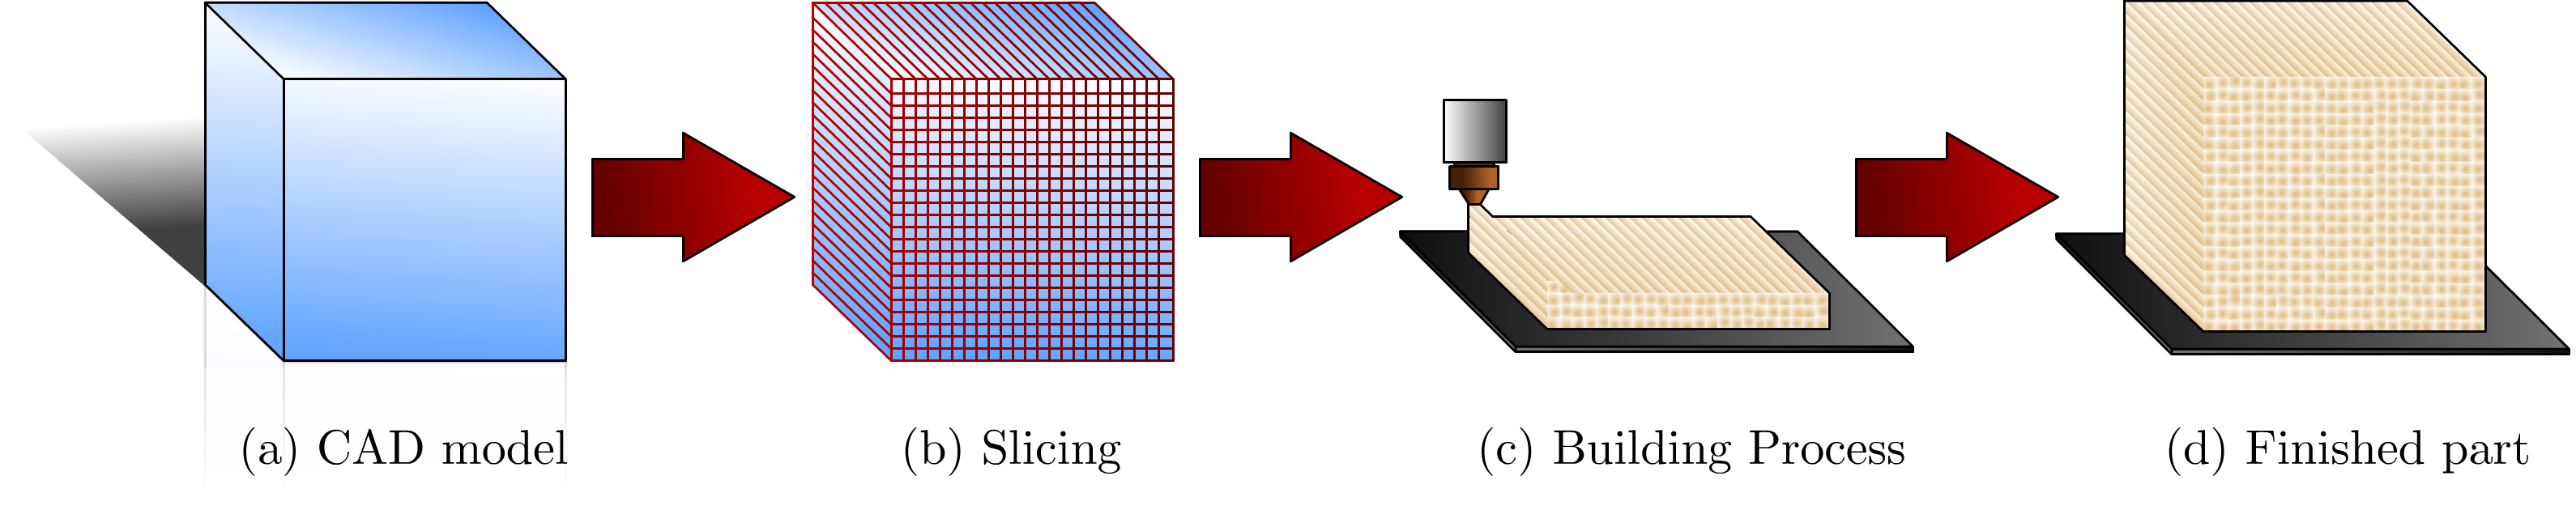
\includegraphics[width=\linewidth]{AM_flowchart_1}
	\caption{Process flow of AM} \label{fig:AM_flow}
\end{figure}
\pagebreak %Used to move the entire paragraph to a new page.
 
While all AM technologies operate on the same basic process flow described above, the specifics of each AM technique vary substantially, ranging from processes that use paper and binder, all the way through metal-based, laser tracing technologies. Since this is a rapidly evolving field, no general consensus exists for classifying the multiple AM processes available. However, the classification system proposed under the ASTM/ISO 52900 standard \cite{ASTM52900}, has been somewhat accepted by the field and divides AM technologies as follows:
\begin{enumerate}
	\item \textbf{Binder Jetting}: AM techniques where a binding agent is used to selectively promote cohesion in powder materials -generally gypsum, sand or metallic powders~\cite{ASTM52900,3DHubs2018}.
	\item \textbf{Directed Energy Deposition}: AM processes where a focused thermal energy source (i.e. laser, electron beam, plasma arc) is used to fuse materials as they are being deposited in the build volume. Materials are almost exclusively metals~\cite{ASTM52900,3DHubs2018}.
	\item \textbf{Material Extrusion}: In this type of AM technology, material is dispensed through a nozzle or orifice. Fused Filament Fabrication belongs to this classification. Materials are almost exclusively thermoplastics \cite{ASTM52900,3DHubs2018}.
	\item \textbf{Material Jetting}: AM techniques where build material is deposited selectively in droplets. Materials are usually wax or thermoplastics, but there are examples of metal-based, material jetting techniques \cite{ASTM52900,3DHubs2018}.
	\item \textbf{Powder Bed Fusion}: AM processes where portions of a powder bed are selectively fused through application of thermal energy. \emph{Selective Laser Sintering} (SLS) belongs to this category. Materials are usually thermoplastic polymers or metals \cite{ASTM52900,3DHubs2018}. 
	\item \textbf{Sheet Lamination}: In this type of AM technology, the final part is formed by bonding sheets of material -usually paper or composites \cite{ASTM52900,3DHubs2018}. 
	\item \textbf{Vat Photopolymerization}: In this AM process, a liquid photopolymer is selectively cured by a light source. \emph{Stereolithography} (SLA), arguably the first AM technology, belongs to this category. Due to the nature of this technique, the only materials used are photopolymers \cite{ASTM52900,3DHubs2018}.
\end{enumerate} 

\subsection{Advantages, Disadvantages and Success Stories}\label{subsec:AMAdDis} 
Since AM processes allow a relatively direct conversion of a CAD model into a constructed object, they were originally exclusively used for prototype development. For this reason, they were initially classified as \textquotedblleft \emph{Rapid Prototyping}\textquotedblright~(RP) technologies. This terminology is still used today, however, it is being superseded by \emph{Additive Manufacturing} since its potential to become a proper fabrication technique exists \cite{Gibson2015}. However, while being capable of quickly jumping from part design to manufacturing is a great advantage, AM has its own set of drawbacks. Table \ref{tab:AM_AdDis} summarizes the most noteworthy set of advantages and disadvantages typical of most AM technologies.

\begin{table}[h]
	\centering
	\caption{Advantages and Disadvantages of Additive Manufacturing}
	\label{tab:AM_AdDis}
	\begin{tabu} to 0.95\textwidth {  X[c]  X[c] }
		\hline
		\textbf{Advantages} & \textbf{Disadvantages} \\ 
		\hline
		Faster product development cycles \cite{Gibson2015} & Part quality highly dependent on process parameters \cite{Gibson2015}\\
		%---------
		No additional tools needed for part fabrication\cite{Gibson2015}&  Stratified build generally results in anisotropic parts \cite{Gibson2015, Capote2017}\\
		%---------
		Cost effective for small batches of parts \cite{Baumers2016,Conner2014,Berman2012}&  Costly for production of more than hundreds of parts \cite{Baumers2016,Conner2014,Berman2012}\\
		\hline
	\end{tabu}
\end{table}   

Out of all the described advantages and disadvantages, the high anisotropy of AM parts is responsible for the slow embrace of AM in highly demanding engineering fields -such as the aerospace and automotive industries. The highly anisotropic mechanical behavior makes it extremely difficult to predict part failure, therefore, it can't be implemented in engineering applications where catastrophic failure is to be avoided at all costs. Even so, success stories of implementation of AM in industrial environments are abundant. Below is a number of relatively 
recent examples:

\begin{itemize}
	\item \textbf{Volkswagen Autoeuropa}: This automotive assembly plant implemented the use of FFF machines to manufacture tools, jigs and fixtures used in their assembly line. They now produce 93\% of the tools that were historically externally sourced, and have reportedly cut their tool development time and costs by 95\% and 91\% respectively \cite{deVries2017}.
	\item \textbf{General Electric}: GE is currently producing in Alabama a complex fuel nozzle injector for the LEAP jet engine, using powder based, metal AM. The complex geometry of this component could not be manufactured by any other manufacturing technique. The production plant is expected to have 50 AM machines producing 35,000 fuel nozzle injectors annually by 2020 \cite{GEAdditive2016}. 
	\item \textbf{Adidas and New Balance}: Both shoe companies have developed separate approaches to constructing highly optimized, 3D printed midsoles for high performance running sneakers. New Balance makes use of SLS technology to build the intricate geometry of their \textquotedblleft \emph{Zante Generate}\textquotedblright~sneaker, using powdered TPU elastomer as the parent material. The designed honeycomb structure of the midsole, combined with the flexible material used, are supposed to improve the comfort and support brought by the shoe \cite{NewBalance2016}. Adidas on the other hand chose to develop the \textquotedblleft \emph{AlphaEDGE 4D LTD}\textquotedblright~running shoe using the CLIP technology by Carbon3D. While the cell geometry in  the midsole is also supposed to bring performance and comfort improvements, the final ambition of Adidas is to perfect the technology to a point where a customer can simply go to a shoe store, have their feet scanned, and receive a fully customized shoe with a 3D printed midsole that fits their particular needs \cite{Matisons2015,Saunders2018}. In both cases, the geometry of the midsole can only be produce by AM. The intricate structures in the midsoles can be seen in Figure \ref{fig:AMshoes}.
		
\end{itemize}
\begin{figure}[h]
	\center
	\subfloat[New Balance Zante Generate~\cite{NewBalance2016}\label{fig:NBZG}]{%
		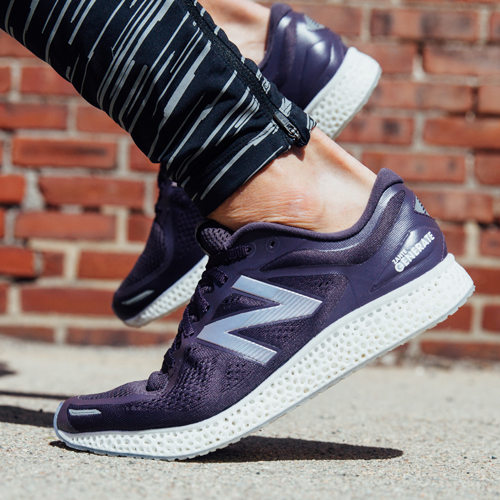
\includegraphics[height=6cm, keepaspectratio]{NB_generate}
	}
	\hfill
	\subfloat[Adidas AlphaEdge 4D LTD~\cite{Saunders2018}\label{fig:adidas}]{%
		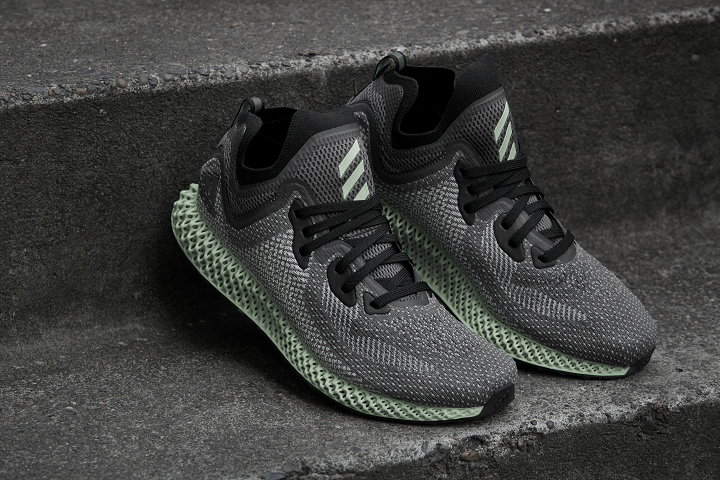
\includegraphics[height=6cm, keepaspectratio]{alphaedge_4D}
	}
	\caption{Shoes with AM midsoles}
	\label{fig:AMshoes}
\end{figure}

Note that in the cases presented, the main reason behind the usage of AM was either reduction expenses associated with producing small batches of parts, or the capability of reproducing a unique and complex geometry. This is a trend that is observed in most of the literature describing implementation of AM into industrial scenarios.

While the advantages and disadvantages described here cover the field of AM as a whole, each technique comes with its own set of pros and cons that may make it the preferred method to reproduce a particular product or geometry. This work, however, focuses solely on FFF. The specifics of this process are described in detail in Section~\ref{sec:FFF}.
\section{Fused Filament Fabrication}\label{sec:FFF} 
\emph{Fused Filament Fabrication}~(FFF) is an AM technology where the final geometry of the part is obtained through controlled extrusion of a liquid, self-hardening material -usually a thermoplastic polymer in molten state \cite{Gibson2015}. Originally developed by Stratasys in the 1980s under the \textendash~still trademarked \textendash~\emph{Fused Deposition Modeling}~(FDM\texttrademark) moniker, it has recently become one of the most widely used AM techniques due to the advent of low-cost, desktop FFF machines in the early 2010s caused by the expiration of key patents from Stratasys \cite{Gibson2015,Capote2017}. 

\pagebreak
\subsection{The FFF process}\label{ssec:FFFmach}

\begin{figure}[h]
	\center
	\subfloat[FFF printhead\label{fig:FFFnoz}]{%
		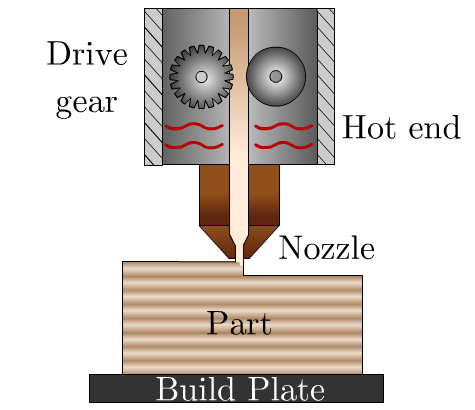
\includegraphics[height=6cm, keepaspectratio]{nozzle}
		}
	\hfill
	\subfloat[Typical FFF machine\label{fig:FFFmach}]{%
		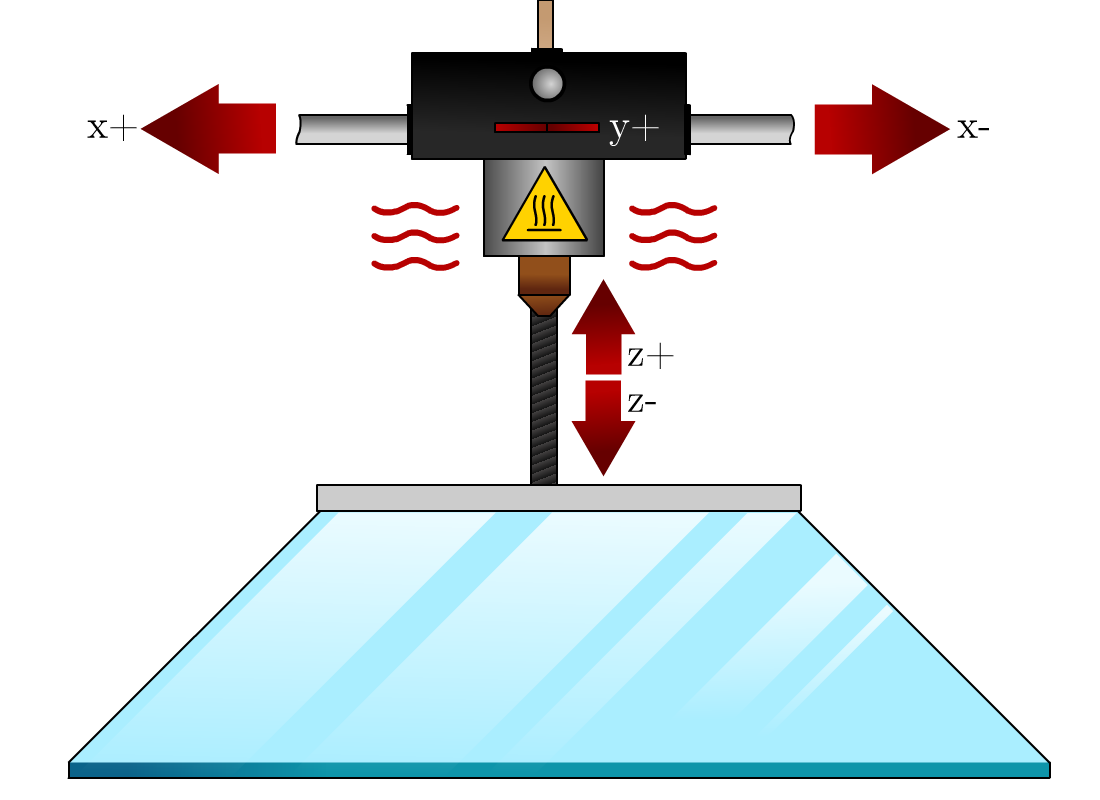
\includegraphics[height=6cm, keepaspectratio]{printer_layout}
		}
	\caption{The typical FFF machine configuration} \label{fig:machconfig}
\end{figure}
Like all AM technologies, the FFF process starts in a computer with a CAD model converted to the \emph{.stl} file format. The geometry is then translated to machine instructions through a \emph{slicing engine}, where the user inputs process parameters. Finally the \emph{toolpath} is executed by the FFF printer, building the object in a layer-by-layer basis -sometimes referred to as \emph{2.5D} printing. Figure \ref{fig:FFFflow} shows an abridged version of the process. The \emph{z} axis indicates the intended build direction. 
\begin{figure}[h]
	\center
	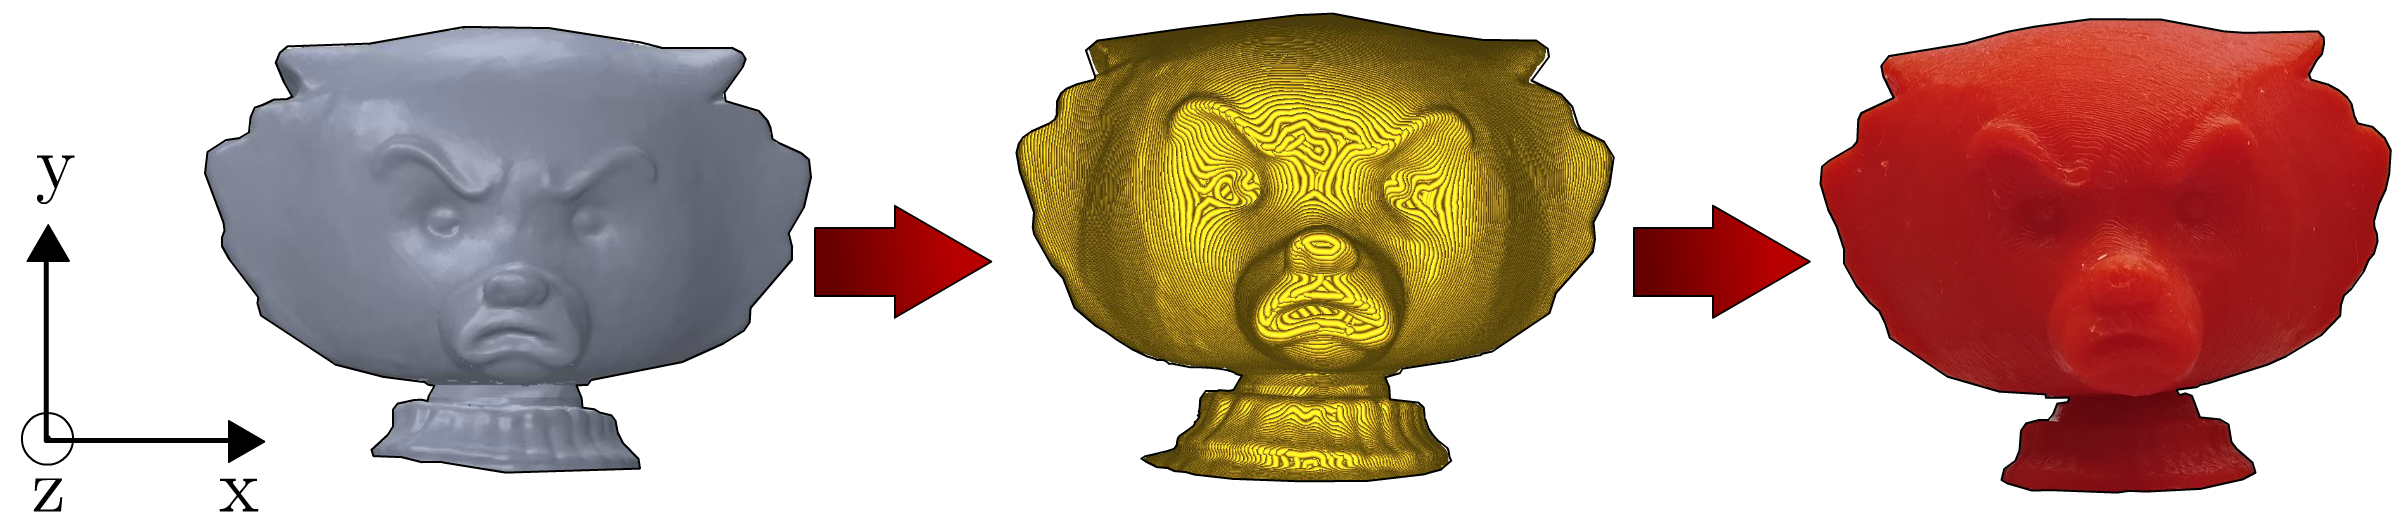
\includegraphics[width=0.95\textwidth]{FFF_flow}
	\caption{From left to right: stl, toolpath and final part} \label{fig:FFFflow}
\end{figure}
%Nomenclature introduced in this chapter:
\nomenclature[A]{SLA}{Stereolithography}% 
\nomenclature[A]{SLS}{Selective Laser Sintering}%
\end{document}
                % oocriterion.tex
\documentclass[main.tex]{subfiles}
\begin{document}
\chapter{A Novel Failure Criterion} \label{ch:oocrit}
\epigraph{\textit{The Osswald$^2$ criterion}}

As described during Section \ref{sec:FC} of Chapter \ref{ch:bg}, currently available failure criteria fail to completely integrate interaction effects into the modeled failure behavior of anisotropic materials. In 2017, Paul and Tim Osswald proposed a model that attempts to overcome these limitiations \cite{Osswald2017a}. This recent failure criterion has the following characteristics:
\begin{itemize}
	\item \textbf{Tensor based and purely mathematical}: as opposed to phenomenological or mechanistic models such as the Puck or Cuntze failure criteria.
	\item \textbf{Based on the Gol'denblat-Kopnov model}.
	\item \textbf{Includes stress interactions that other models neglect}.
\end{itemize}

Originally titled \textquotedblleft A Strength Tensor Based Failure Criterion with Stress Interactions\textquotedblright, it will be referred in this work as the Osswald-Osswald Criterion (OOC). This chapter will describe the Gol'denblat-Kopnov model upon which the OOC is based, followed by a proper description of how this novel model implements stress interactions.

\section{The Gol'denblat-Kopnov Model}\label{sec:GKC}
The Gol'denblat-Kopnov Criterion (GKC) describes a mathematical function that depends on the stress state of an anisotropic material. Should the computation of this expression exceed a threshold, part failure is to be expected. To that end, a scalar function that depends on stress tensors that completely characterize the state of the material was developed \cite{Goldenblat1965}. This function is shown in Equation \ref{eq:GKCgen}, where stresses are denoted $\sigma$, and the subindices \emph{i,j,k,l} denote a particular load direction.

\begin{equation} \label{eq:GKCgen}
f=(F_{ij}\sigma_{ij})^\alpha + (F_{ijkl}\sigma_{ij}\sigma_{kl})^\beta + (F_{ijklmn}\sigma_{ij}\sigma_{kl}\sigma_{mn})^\gamma + ...
\end{equation}

The terms $F_{ij}$, $F_{ijkl}$ and $F_{ijklmn}$ represent second, fourth and sixth order tensors respectively. These terms of the equation depend on engineering strength parameters, such as the ultimate tensile and compressive strengths of the material in a particular load direction \cite{Osswald2017a}. Due to the complexity associated with using higher order tensors, Gol'denblat and Kopnov limited their approach to using only the second and fourth order terms. Thus Equation \ref{eq:GKCgen} is reduced to:

\begin{equation} \label{eq:GKCgenTrunc}
f=(F_{ij}\sigma_{ij})^\alpha + (F_{ijkl}\sigma_{ij}\sigma_{kl})^\beta
\end{equation}

In order to attain a linear criterion scalar function, the exponents $\alpha$ and $\beta$ were assigned values of 1 and 1/2 respectively. Finally, in plane stress scenarios, the GKC becomes:

\begin{equation} \label{eq:GKCfinal}
\begin{split}
f=F_{11}\sigma_{11} + F_{22}\sigma_{22} + F_{12}\tau_{12} + (F_{1111}\sigma_{11}^{2} + F_{2222}\sigma_{22}^{2} + F_{1212}\tau_{12}^{2} \\ + 2F_{1122}\sigma_{11}\sigma_{22} + 2F_{1112}\sigma_{11}\tau_{12} + 2F_{2212}\sigma_{22}\tau_{12})^{1/2}
\end{split}
\end{equation}

Note that in Equation \ref{eq:GKCfinal} $\sigma$ and $\tau$ denote normal and shear stresses respectively. Figure \ref{fig:loaddir} depicts an anisotropic material and all the possible loading directions for reference.

\begin{figure}[h]
	\center
	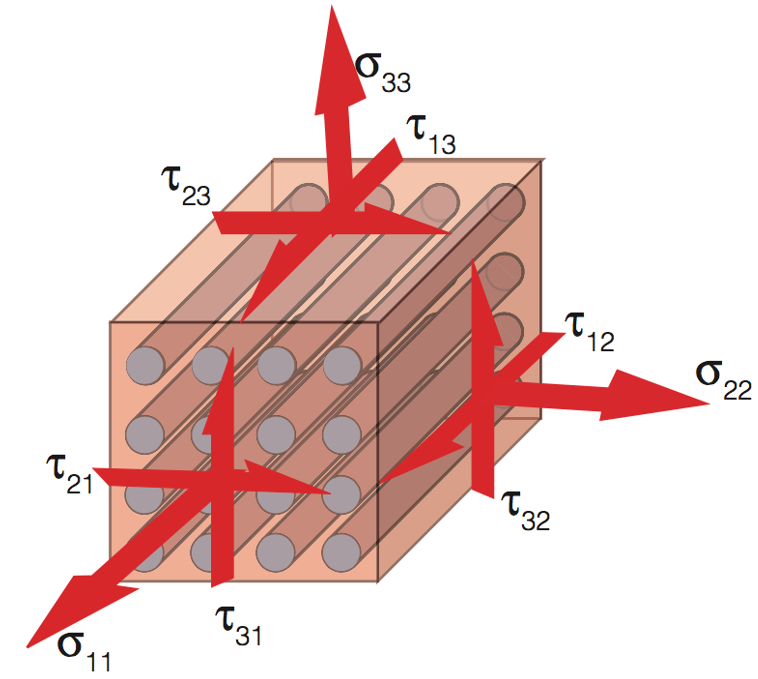
\includegraphics[height=5cm]{reference_cube}
	\caption{Different load directions in an anisotropic material} \label{fig:loaddir}
\end{figure}

Per Gol'denblat and Kopnov's design, should the computation of $f$ in Equation \ref{eq:GKCfinal} be greater or equal to 1, part failure is to be expected. However, to simplify calculations, they deliberately assumed the interaction terms $F_{1112}$ and $F_{2212}$ to be zero. This is an important consideration that will come into play when describing the OOC.

Most of the terms in the GKC are obtained through mechanical testing of coupons under pure uniaxial loads in the 1 or 2 direction, or pure shear in the 1-2 plane \cite{Osswald2017a}. In these scenarios, $f$ will be equal to 1 at failure, and the stress state will be known to the user, allowing some of the unknown tensorial parameters to be easily calculated. Using $F_{11}$ and $F_{1111}$ as examples, the process would be as follows:
\pagebreak
\begin{enumerate}
	\item The tensile and compressive strength in the 1-1 direction would be obtained through mechanical testing. These values are named $X_t$ and $X_c$ respectively.
	\item Under these failure conditions, Equation \ref{eq:GKCfinal} is reduced to the following system of equations:
	\[
	\systeme*{1=F_{11}X_t + (F_{1111}X_t^{2})^{1/2}, 1= -F_{11}X_c + (F_{1111}X_c^{2})^{1/2}}
	\]

	\item $F_{11}$ and $F_{1111}$ can be obtained, yielding $F_{11}=\frac{1}{2}(\frac{1}{X_t}-\frac{1}{X_c})$ and $F_{1111}=\frac{1}{4}(\frac{1}{X_t}+\frac{1}{X_c})^2$.
\end{enumerate}

The only exception to this procedure would be the $F_{1122}$ component, which requires measuring the positive and negative shear strengths of a coupon with reinforcement oriented in 45$^\circ$. These parameters are named $S_{45p}$ and $S_{45n}$ respectively. Table \ref{tab:GKparam} summarizes the nomenclature used for the strength parameters required to completely populate the failure function of the GKC. Table \ref{tab:GKtens} summarizes all the tensorial component calculations.

\begin{table} [h]
	\centering
	\caption{Nomenclature of the GKC parameters}
	\begin{tabular}{ c c }
	\toprule
		\textbf{Parameter} & \textbf{Description} \\ 
		\midrule
		$X_t$ & Tensile strength in the 1-1 direction\\
		$X_c$ & Compressive strength in the 1-1 direction\\
		$Y_t$ & Tensile strength in the 2-2 direction\\
		$Y_c$ & Compressive strength in the 2-2 direction\\
		$S_{45p}$ & Positive shear strength for 45$^\circ$ specimen\\
		$S_{45n}$ & Negative shear strength for 45$^\circ$ specimen\\
		$S$ & Shear strength in the 1-2 plane\\
	\bottomrule
	\end{tabular}
	\label{tab:GKparam}
\end{table}

\begin{table} [h]
	\centering
	\caption{Tensorial components of the GKC}
	\begin{tabular}{ c c } 
	\toprule
		\textbf{Component} & \textbf{Formula} \\
		\midrule
		$F_{11}$ & $\frac{1}{2}(\frac{1}{X_t}-\frac{1}{X_c})$\\ [1ex]
		$F_{1111}$ & $\frac{1}{4}(\frac{1}{X_t}+\frac{1}{X_c})^2$\\ [1ex]
		$F_{22}$ & $\frac{1}{2}(\frac{1}{Y_t}-\frac{1}{Y_c})$\\ [1ex]
		$F_{2222}$ & $\frac{1}{4}(\frac{1}{Y_t}+\frac{1}{Y_c})^2$\\ [1ex]
		$F_{12}$ & 0\\ [1ex]
		$F_{1212}$ & $\frac{1}{S^2}$\\ [1ex]
		$F_{1122}$ & $\frac{1}{8}[(\frac{1}{X_t}+\frac{1}{X_c})^2+(\frac{1}{Y_t}+\frac{1}{Y_c})^2-(\frac{1}{S_{45p}}+\frac{1}{S_{45n}})^2]$\\ [1ex]
		\bottomrule
	\end{tabular}
	\label{tab:GKtens}
\end{table}
\pagebreak

\section{The Osswald-Osswald Criterion}\label{sec:OOC}
One of the assumptions made in the GKC is that the components $F_{1112}$ and $F_{2212}$ in Equation \ref{eq:GKCfinal} are null. While this simplifies the model, it essentially neglects any interactions between axial loads and shear stresses, namely, the $\sigma_{11}$ - $\tau_{12}$ and $\sigma_{22}$ - $\tau_{12}$ interactions. Practically, this causes the failure surface developed through the GKC to under predict shear strengthening effects exhibited by anisotropic materials loaded in combined axial and shear conditions. Figure \ref{fig:GKClimit} shows a comparison between experimental data obtained from the first World Wide Failure Exercise (WWFE-I) and the GKC envelope developed for this material. In this example, a unidirectional glass reinforced epoxy composite was tested in multiple loading conditions in the $\sigma_{22}$ and $\tau_{12}$ stress plane. White circles indicate average values for pure uniaxial or shear scenarios. Note how on the first quadrant, the model follows the data closely. However, in the second quadrant, the criterion is relatively conservative, failing to capture the strengthening that occurs when loading the material in compression and shear.   

\begin{figure}[h]
	\center
	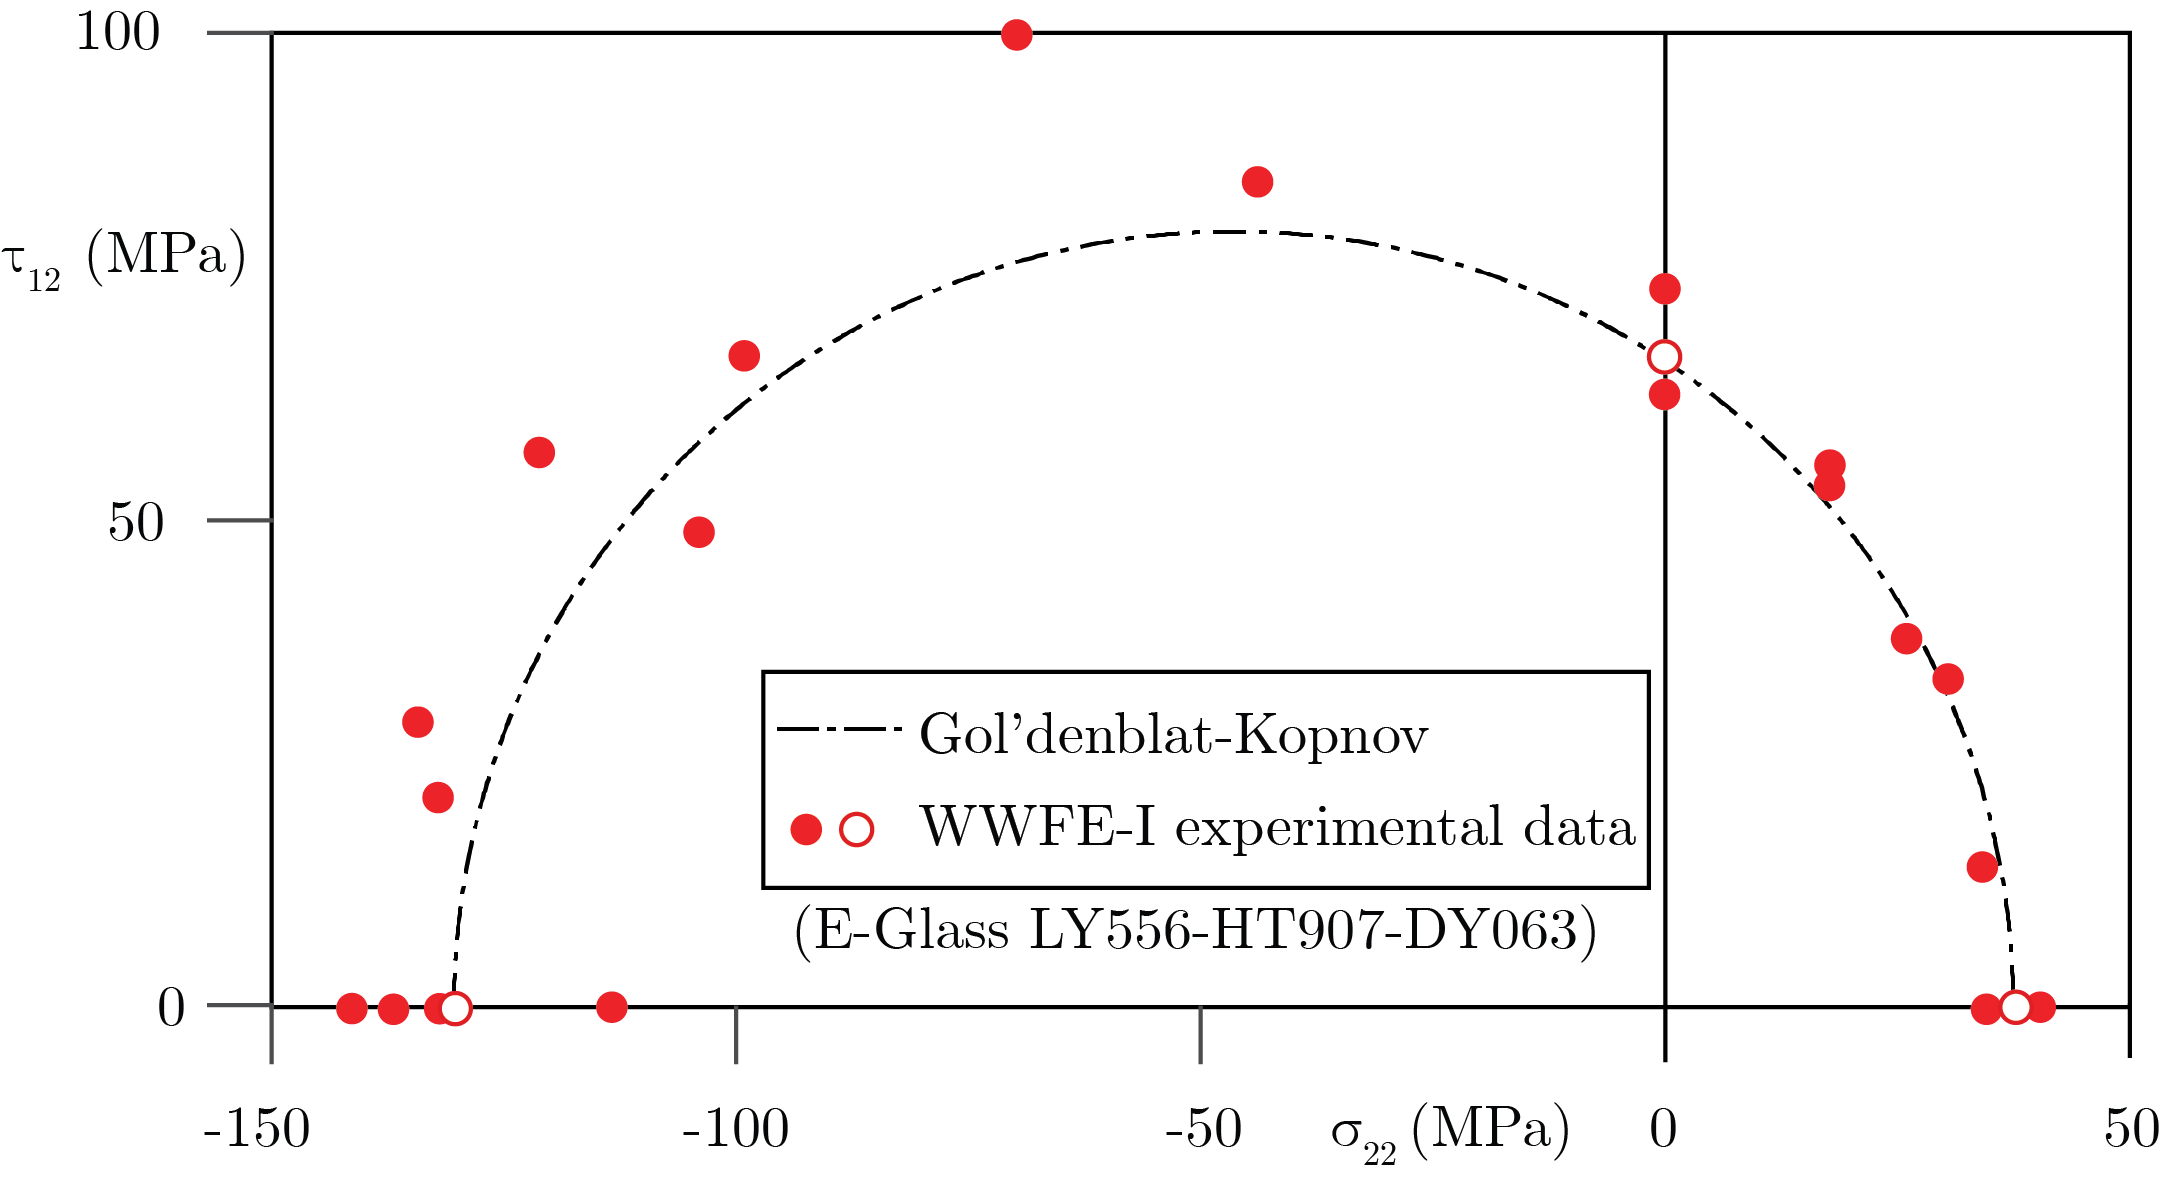
\includegraphics[height=7cm]{GK_thesis}
	\caption{GKC failure surface developed using data from the WWFE-1 \cite{Osswald2017a}} \label{fig:GKClimit}
\end{figure}

The Osswald-Osswald Criterion (OOC) attempts to overcome these limitations by building upon the GKC. For the OOC, the interaction effects are captured through the use of the slopes of the failure surface at any of the points where the engineering strength is known within a particular stress plane \cite{Osswald2017a}. In this failure scenario, the stress state of the coupon is known and easy to implement into Equation \ref{eq:GKCfinal}, where $f=1$. The resulting expression can then be derived with respect to one of the stresses, allowing for the interaction components to be calculated. This is better illustrated through an example. Assuming the component of interest is $F_{2212}$, the procedure to calculate it through the OOC would be as follows:

\pagebreak
\begin{enumerate}
	\item Obtain all the tensorial components possible through the GKC.
	\item Using the $\sigma_{22}$\textendash$\tau_{12}$ stress plane, take the derivative of Equation \ref{eq:GKCfinal} as a function of $\sigma_{22}$ in the scenario of failure under pure shear ($f=1$). This yields the expression:
	\begin{equation} \label{eq:OOCex1}
	 0= F_{22}+[F_{1212}S(\frac{d\tau_{12}}{d\sigma_{22}})+F_{2212}S]
	\end{equation}
	 where $\frac{d\tau_{12}}{d\sigma_{22}}$  is the slope of the graph at failure under shear. This term is named $\mu^{2212}$ in the OOC and can be obtained by performing combined loading tests. Refer to Figure \ref{fig:OOCdemo} for a visual representation.
	\item Rearranging Equation \ref{eq:OOCex1} to solve for the unknown $F_{2212}$ gives the following expression:
	\begin{equation} \label{eq:OOCex2}
	F_{2212}=-\frac{F_{22}}{S}-F_{1212}\mu^{2212}
	\end{equation}
\end{enumerate}

\begin{figure}[h]
	\center
	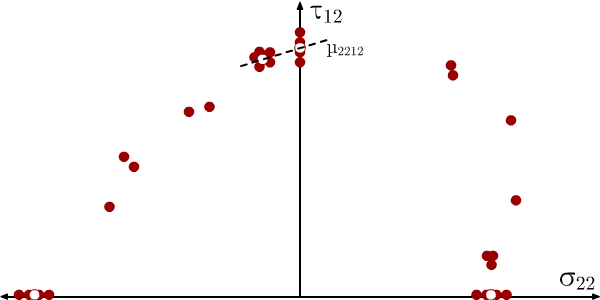
\includegraphics[height=5cm]{OOC_demo_thesis}
	\caption{$\mu^{2212}$ parameter in the $\tau_{12}$ - $\sigma_{22}$ plane} \label{fig:OOCdemo}
\end{figure}

A similar procedure can be followed for any $\sigma_{ii}$-$\tau_{ij}$ interaction, or even any $\sigma_{ii}$-$\sigma_{jj}$ components. For this last scenario, the user has four potential choices of slopes to determine the tensorial component of interest. In the OOC, any slope obtained from a $\sigma_{ii}$-$\sigma_{jj}$ stress plane is named $\lambda^{iijj}$, as opposed to $\mu^{iiij}$ for slopes in a $\sigma_{ii}$-$\tau_{ij}$ reference. A schematic of all possible $\lambda^{iijj}$ is shown in Figure \ref{fig:OOCdemo2}, while Table \ref{tab:OOCcomp} summarizes all the possible interaction factors available through the OOC, where $\tau_{ij}^u$ denotes ultimate shear strength in a particular shear plane. 

\pagebreak
\begin{figure}[h]
	\center
	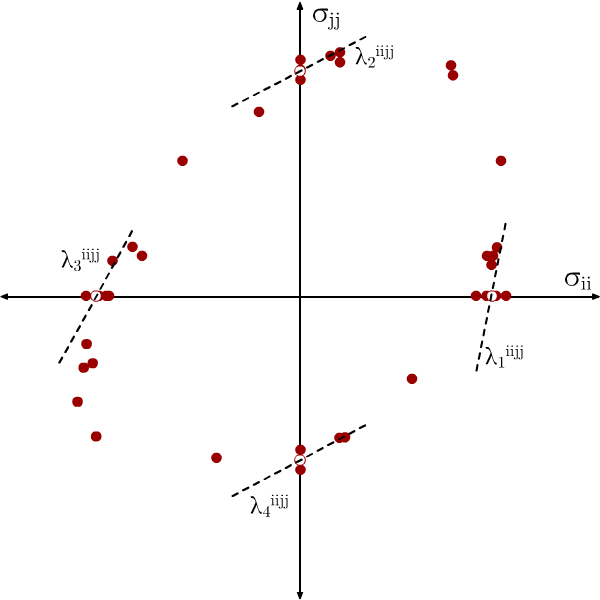
\includegraphics[height=10cm]{OOC_demo_thesis2}
	\caption{$\lambda^{iijj}$ parameters in a generic $\sigma_{ii}$ - $\sigma_{jj}$ stress plane} \label{fig:OOCdemo2}
\end{figure}
\begin{table}[!htbp] %Fixates table so that it doesn't randomly jump around between pages
	\renewcommand{\arraystretch}{1.5}
	\centering
	\caption{Interaction components attainable through the OOC~\cite{Osswald2017a}}
	\begin{tabular}{ c c } 
		\toprule
		\textbf{Component} & \textbf{Formula} \\
		\midrule
		$F_{iiij}$ & $-\frac{F_{ii}}{\tau_{ij}^u}-F_{ijij}\mu^{iiij}$\\
		$F_{iijj}$ through $\lambda^{iijj}_1$ & $-\frac{(F_{ii}+F_{jj}\lambda^{iijj}_1)F_{iiii}^{1/2}+F_{iiii}}{\lambda^{iijj}_1}$\\
		$F_{iijj}$ through $\lambda^{iijj}_2$ & $-(F_{ii}+F_{jj}\lambda^{iijj}_2)F_{jjjj}^{1/2}-F_{jjjj}\lambda^{iijj}_2$\\
		$F_{iijj}$ through $\lambda^{iijj}_3$ & $\frac{(F_{ii}+F_{jj}\lambda^{iijj}_3)F_{iiii}^{1/2}-F_{iiii}}{\lambda^{iijj}_3}$\\
		$F_{iijj}$ through $\lambda^{iijj}_4$ & $(F_{ii}+F_{jj}\lambda^{iijj}_4)F_{jjjj}^{1/2}-F_{jjjj}\lambda^{iijj}_4$\\
		\bottomrule
	\end{tabular}
	\label{tab:OOCcomp}
\end{table}

Applying the OOC to the data shown in Figure \ref{fig:GKClimit} demonstrates how the failure surface developed through this new criterion better reflects the failure behavior than its GKC counterpart. A comparison between the two can be seen in Figure \ref{fig:GKOOComp}. Note how the OOC envelope captures the shear strengthening better than the GKC. 
\begin{figure}[h]
	\center
	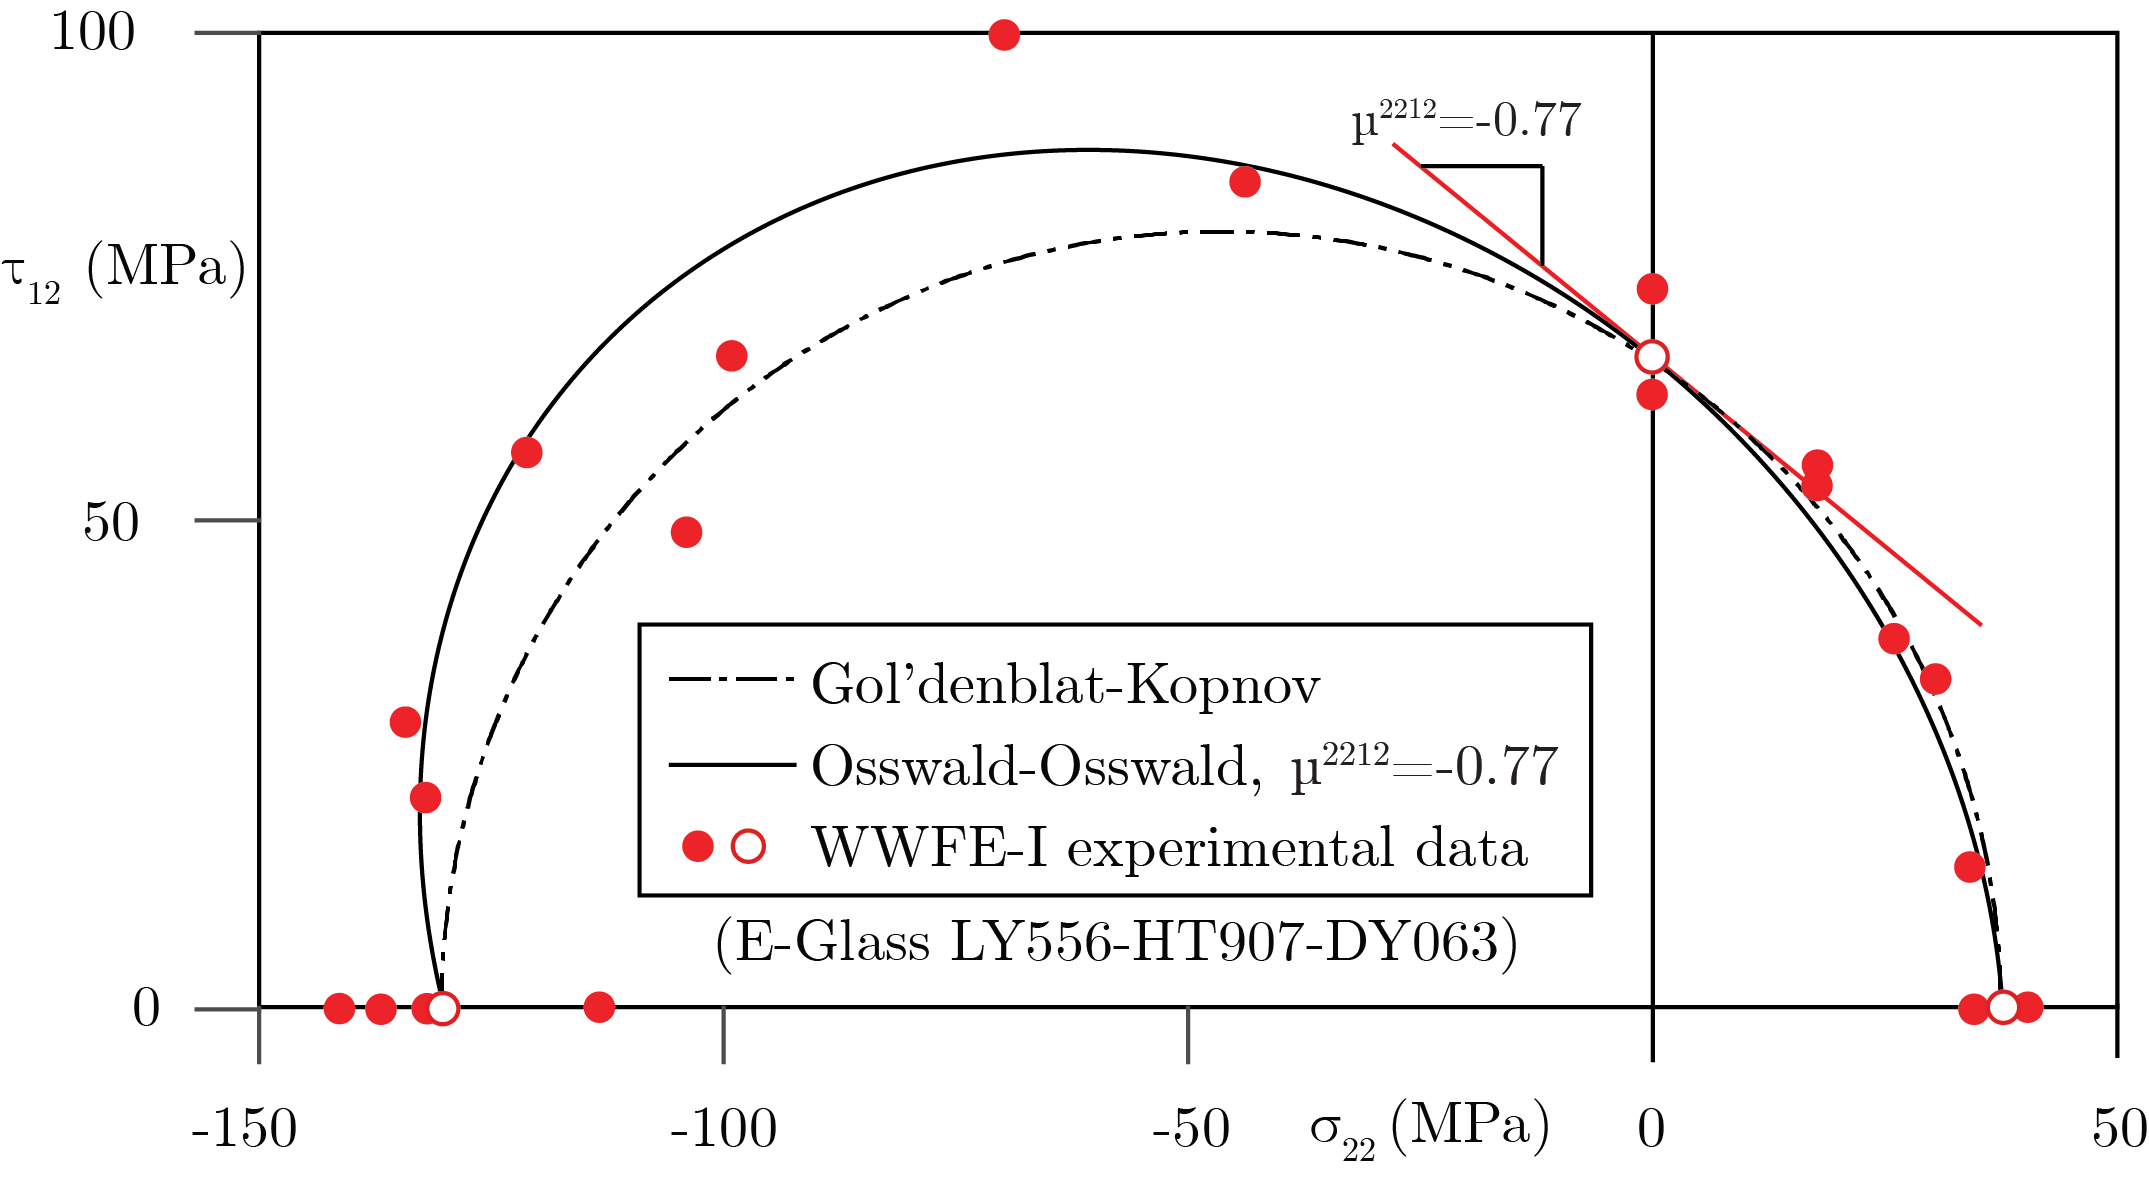
\includegraphics[height=7cm]{GK_OO}
	\caption{Comparison of GKC and OOC failure envelopes \cite{Osswald2017a}} \label{fig:GKOOComp}
\end{figure}

The OOC offers a way of capturing in a more accurate manner the different failure modes of parts produced through AM technologies. As an example, the model has been successfully implemented by Obst \emph{et al.} in 2018 for SLS manufactured parts produced with PA12 \cite{Obst2018, Obst2017}. Their results show how the model was able to capture the $\tau_{12}$-$\sigma_{22}$ and $\sigma_{11}$-$\sigma_{22}$ interactions. The failure surface obtained is shown in Figure \ref{fig:OOCSLS}.

\begin{figure}[h]
	\center
	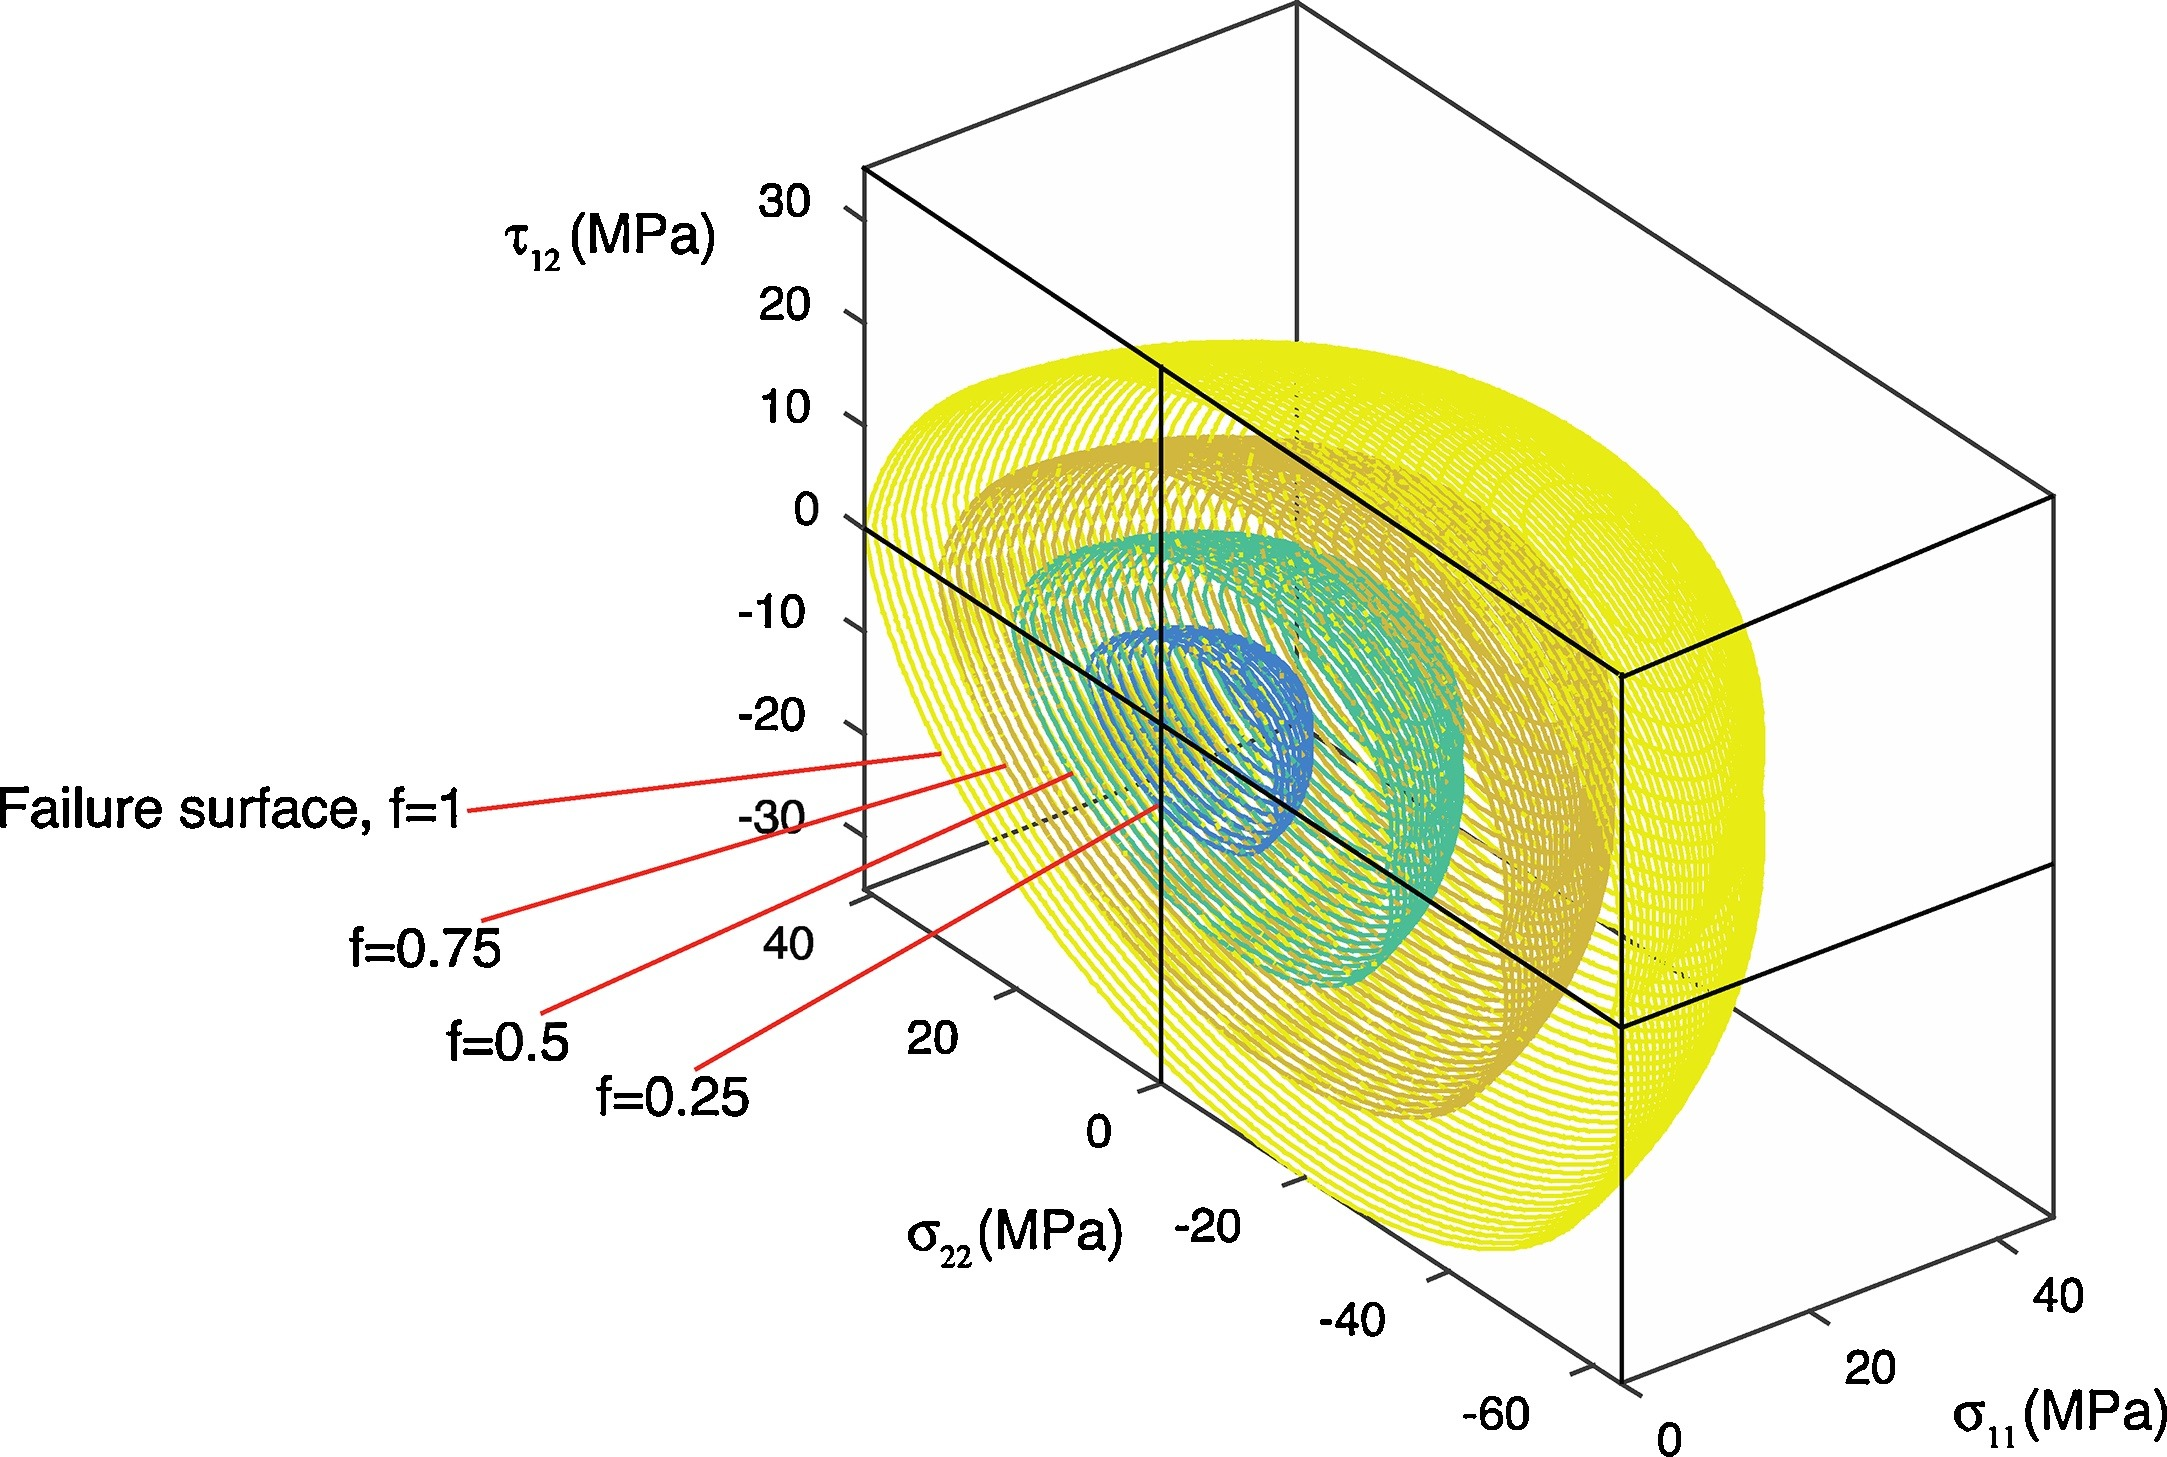
\includegraphics[height=7cm]{Obst_SLS}
	\caption{Failure surface for SLS developed through the OOC \cite{Obst2018}} \label{fig:OOCSLS}
\end{figure}

This work will apply the OOC to FFF, in the hopes that it becomes a tool for safely designing parts intended to be manufactured through this process. Chapter \ref{ch:exp} will detail the material and experimental methods used to achieve this goal.
  
% Nomenclature introduced in this chapter:
\nomenclature[A]{OOC}{Osswald-Osswald Criterion}% 
\nomenclature[A]{GKC}{Gol'denblat-Kopnov Criterion}% 

% Symbols introduced in this chapter:
\nomenclature[S]{$X_t$}{Tensile strength in the 1-1 direction \nomunit{$MPa$}}
\nomenclature[S]{$X_c$}{Compressive strength in the 1-1 direction \nomunit{$MPa$}}
\nomenclature[S]{$Y_t$}{Tensile strength in the 2-2 direction \nomunit{$MPa$}}
\nomenclature[S]{$Y_c$}{Compressive strength in the 2-2 direction \nomunit{$MPa$}}
\nomenclature[S]{$S$}{Shear strength in the 1-2 plane \nomunit{$MPa$}}
\nomenclature[S]{$S_{45p}$}{Positive shear strength for 45$^\circ$ specimen \nomunit{$MPa$}}
\nomenclature[S]{$S_{45n}$}{Negative shear strength for 45$^\circ$ specimen \nomunit{$MPa$}}
\nomenclature[S]{$\mu^{1112}$}{OOC parameter- slope at pure shear failure in the $\sigma_{11}$ - $\tau_{12}$ plane \nomunit{$-$}}
\nomenclature[S]{$\mu^{2212}$}{OOC parameter- slope at pure shear failure in the $\sigma_{22}$ - $\tau_{12}$ plane \nomunit{$-$}}
\end{document}
                % experimental.tex
\documentclass[main.tex]{subfiles}
\begin{document}
\chapter{Experimental Methods} \label{ch:exp}
This chapter explains all the experimental procedures followed to obtain all the parameters necessary to compute the failure surface described by the OOC. This includes detailed information pertaining to the material used, sample geometries and toolpath considerations, as well as describing the equipment used to produce and test the coupons.   

\section{Material} \label{sec:material}

The first step of the experimental work involved development of a custom thermoplastic filament for the FFF process. The reasoning behind this decision was two-fold. First, the use of an off the shelf, commercial thermoplastic filament generally does not guarantee that two different spools were produced under the same processing conditions \textemdash or even using the same parent material. Secondly, the results from Koch \emph{et al.} \cite{Koch2017} show that fluctuations in the filament diameter have an impact in the mechanical properties of FFF parts due to improper volumetric output at the nozzle.

The Cycolac\textregistered~MG94 material produced by SABIC was chosen for this work. This is an Acrylonitrile Butadiene Styrene (ABS) based material traditionally used for injection molding thin walled parts, as well as extrusion of FFF filament. With a reported Melt Flow Index of 11.7 g/10 min, it is an ideal material for both the FFF and extrusion processes. The MG94 was extruded in a setup that consisted of a single screw extruder (Extrudex EDN 45X30D, Germany) with 45 mm screw diameter and L/D ratio of 30D. The hot melt was extruded at 205 $^\circ$C through a circular die with a 5.8 mm diameter, and then guided through a pre-skinner into a vacuum-assisted, heated water bath (Conair, USA) to cool the extrudate whilst minimizing void formation. The solidified filament was then passed through a 3-axis laser micrometer (LaserLinc, USA) and a belt puller (Conair, USA) configured in a control loop. The dimensions of the filament were controlled by automatically adjusting the speed of the puller if the readings from the micrometer were out of specification \textemdash in this case a diameter of 2.85 mm with a tolerance of $\pm$ 0.02 mm. Finally, the product was wound onto spools using a filament winder. A schematic of the extrusion setup can be seen in Figure \ref{fig:extrLine}. Prior to any usage in a printer, the filament was dried in a silo (Novatec, USA) at 82~$^\circ$C for 3 hours.

\begin{figure}[h]
	\center
	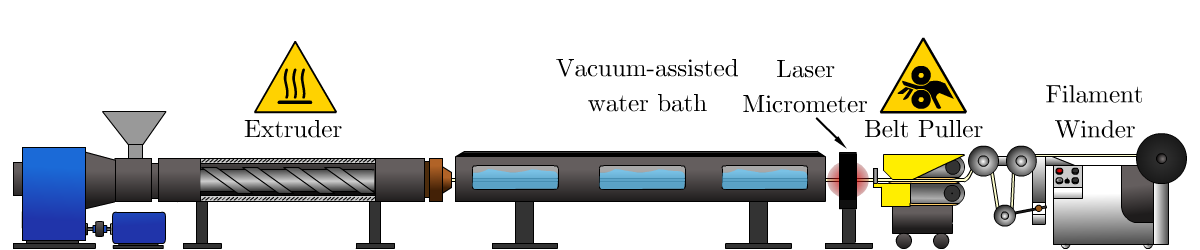
\includegraphics[width=\linewidth]{Extrusion_line}
	\caption{Extrusion line setup} \label{fig:extrLine}
\end{figure}
\pagebreak

\section{Sample Preparation}

As explained in Chapter \ref{ch:oocrit}, the OOC requires mechanical tests to obtain the multiple tensorial components of the mathematical function that describes part failure. Table \ref{tab:testsum} summarizes the tests required.
\begin{table} [h]
\centering
\caption{Mechanical tests required for the OOC}
\begin{tabular}{ c c } 
	\toprule
	\textbf{Mechanical Test} & \textbf{OOC parameters obtained} \\
	\midrule
	Tensile           &   $X_t$, $Y_t$\\
	Compressive       &   $X_c$, $Y_c$\\
	Torsion           &   $S$, $S_{45p}$ , $S_{45n}$\\
	Combined loading  &   $\mu^{1112}$ , $\mu^{2212}$\\
 	\bottomrule
\end{tabular}
\label{tab:testsum}
\end{table}

Given that at the moment of this writing AM testing standards are still in development, custom specimen geometries had to be created in order to test certain loading conditions. Additionally, some bead orientations required are difficult or impossible to reproduce through \emph{2.5-D} FFF. Therefore, the use of a customized robotic, off-axis FFF printer was necessary. This section will detail the coupon geometries used to perform all the mechanical tests described in Table \ref{tab:testsum}, as well as the printing equipment, and toolpath considerations necessary to properly arrange the printed beads in the desired orientation for each condition. 

\subsection{Printing Equipment}
Specimens were produced using either a commercially available desktop FFF printer (Lulzbot TAZ5, USA), or a customized 6-axis robotic printing solution whenever the bead orientation was hard to achieve using a \emph{2.5-D} machine. The robotic printer, developed in the Polymer Engineering Center and nicknamed \emph{Otto} \cite{VanHulle2017}, was based on a 6-axis robot (ABB IRB-120, Switzerland) and fitted with a stationary printhead mounted on an aluminum frame, chosen to be the same extruder from the traditional printer (LulzBot TAZ Single Extruder Tool Head v2, 0.5 mm nozzle, USA) to minimize machine influence on the results. The printing equipment can be seen in Figure \ref{fig:PrintEquip}. 
\begin{figure}[h]
	\center
	\subfloat[TAZ 5 Printer \cite{Lulzbot2018}\label{fig:taz5}]{%
		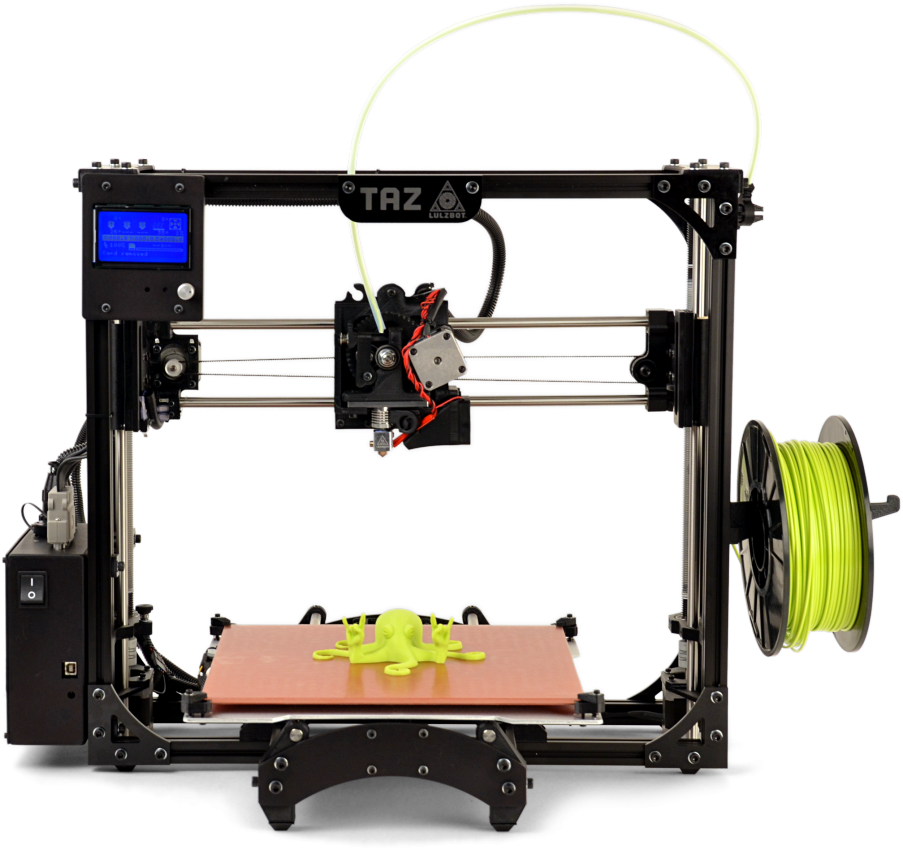
\includegraphics[height=6cm, keepaspectratio]{TAZ_5}
	}
	\hfill
	\subfloat[6-axis robotic printer: \emph{Otto}\label{fig:Otto}]{%
		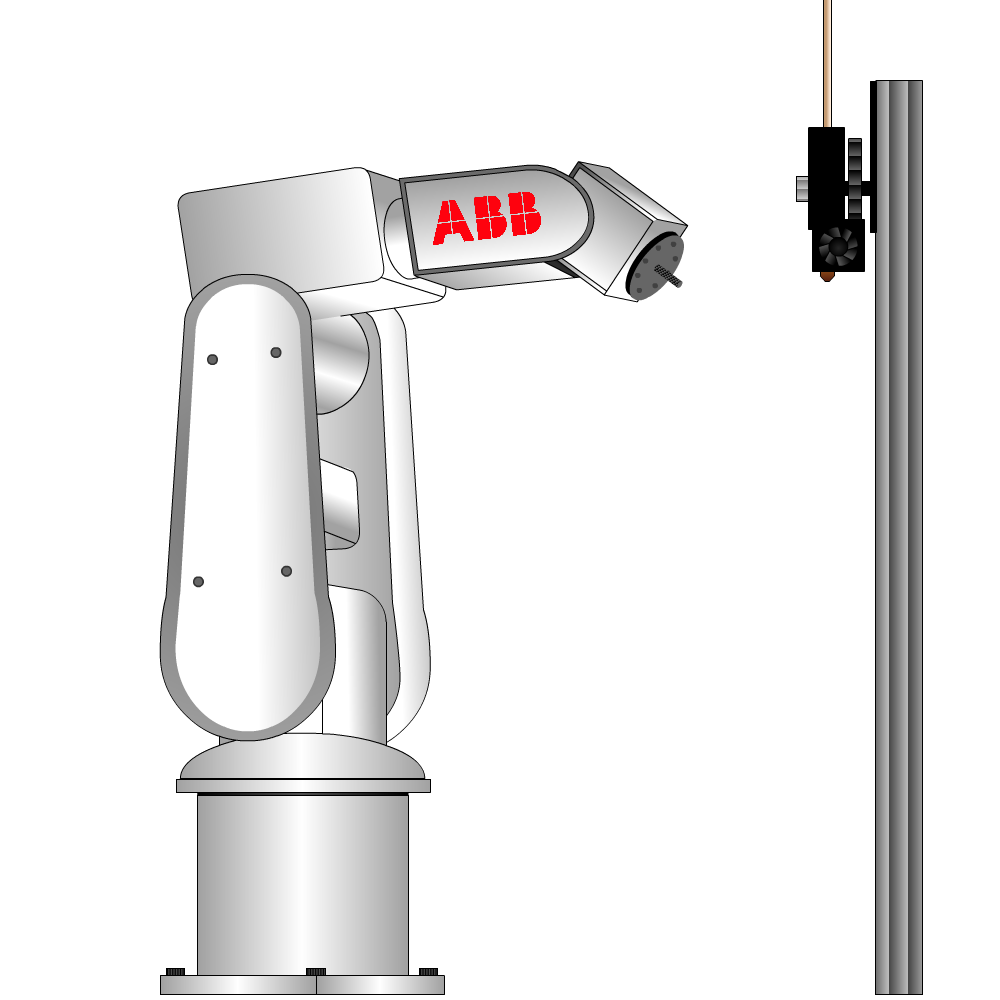
\includegraphics[height=6cm, keepaspectratio]{Otto}
	}
	\caption{Printing equipment} \label{fig:PrintEquip}
\end{figure}

The 6-axis robotic printer's layout is optimized to produce objects of cylindrical nature. A specialized base plate is attached to the sixth axis of the robot, where a threaded rod allows the attachment of disposable plastic cylinders that acts as a build surface. A cylindrical core can then be built by \emph{Otto}, upon which beads in any orientation can be deposited after the robot reorients its joints. Refer to Figure \ref{fig:otto2} for a representation of the process. The left side shows the core being produced atop the disposable build surface, followed by the right hand side, where beads are being laid upon the core in a 45$^\circ$ angle.  
\begin{figure}[h]
	\center
	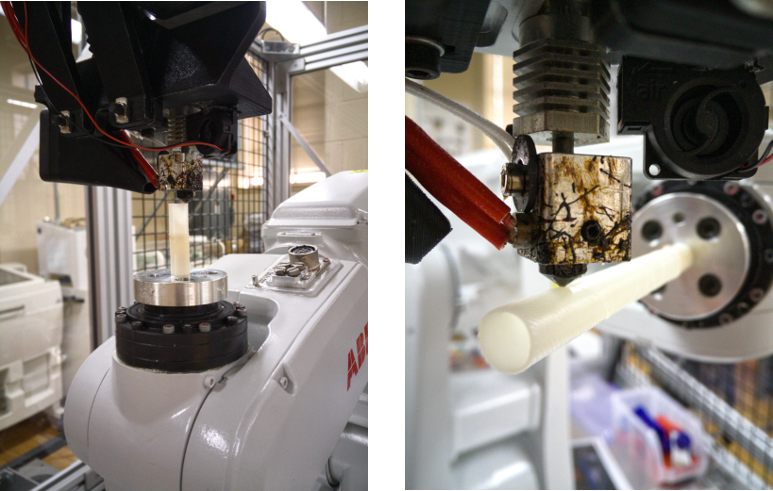
\includegraphics[height=7.5cm, keepaspectratio]{otto2}
	\caption{Print process in \emph{Otto}} \label{fig:otto2}
\end{figure}

Since printing parameters in FFF are known to impact in varying degrees the mechanical performance of objects manufactured through this technology, a conscious effort was made to keep as many processing parameters as possible constant. Table \ref{tab:printparam} summarizes these values.

\begin{table}[!htbp] %Fixates table so that it doesn't randomly jump around between pages
	\renewcommand{\arraystretch}{1.2}
	\centering
	\caption{Constant printing parameters}
	\begin{tabular}{ c c } 
		\toprule
		\textbf{Printing Parameter} & \textbf{Value} \\
		\midrule
		Nozzle temperature & 220$^\circ$C\\
		Bed temperature~\tablefootnote{Applicable only to prints performed on the traditional FFF printer.} & 100$^\circ$C\\
		Printing Speed & 2000 $\frac{mm}{min}$\\
		Layer height & 0.2 mm\\
		Path width & 0.5 mm\\
		Extrusion Factor & 1\\
		\bottomrule
	\end{tabular}
	\label{tab:printparam}
\end{table}

Extrusion Factor (EF) refers to a ratio of the area occupied by the cross section of a bead ($A_{bead}$) divided by the product of the bead width ($W_{bead}$) with the layer height ($H_{layer}$). This factor is used to calculate the length of filament ($L_{fil}$) necessary to produce a bead of known length ($L_{bead}$) as shown in Equations \ref{eq:EFdef} and \ref{eq:EFvol}. The cross sectional area of the filament ($A_{fil}$) is known through the filament diameter used by the printer.

\begin{equation} \label{eq:EFdef}
EF=\frac{A_{bead}}{W_{bead}\times H_{layer}}
\end{equation}  

\begin{equation}\label{eq:EFvol}
\frac{L_{fil}}{L_{bead}}\times A_{fil}=EF \times W_{bead} \times H_{layer}
\end{equation}

   
\subsection{Tensile Specimens}
Tensile coupons were manufactured on the TAZ5, with bead orientations of 0$^\circ$ and 90$^\circ$ with respect to the load direction in order to test $X_t$ and $Y_t$ respectively. The chosen geometry was the ASTM D-638 Type I coupon \cite{ASTMD638} which can be seen in Figure \ref{fig:db}. The toolpath required to produce these samples was developed through \emph{SciSlice}, a customized slicing engine created in the Polymer Engineering Center that allows layer-by-layer and part-by-part controls of crucial process parameters \textemdash such as the bead orientation \textemdash making it ideal for research in the field of FFF \cite{VanHulle2017a}.
\pagebreak
\begin{figure}[h]
	\center
	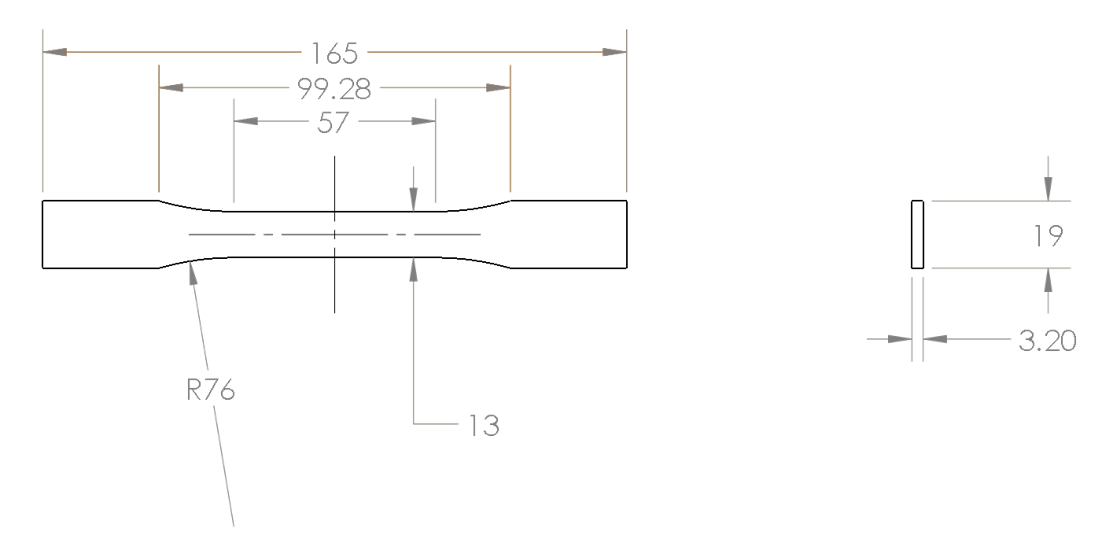
\includegraphics[width=0.95\linewidth, keepaspectratio]{typeIDB}
	\caption{ASTM D-638 Type I coupon} \label{fig:db}
\end{figure}

In order to minimize stress concentrators due to printing discontinuities, the 0$^\circ$ specimens were printed using 13 perimeters, also known as \emph {shells}. This produced a continuous toolpath with beads oriented in the loading direction at the neck section of the specimen. No shells were added to the 90$^\circ$ samples. Refer to Figure \ref{fig:090db} for a visual representation of the coupons. 

\begin{figure}[h]
	\center
	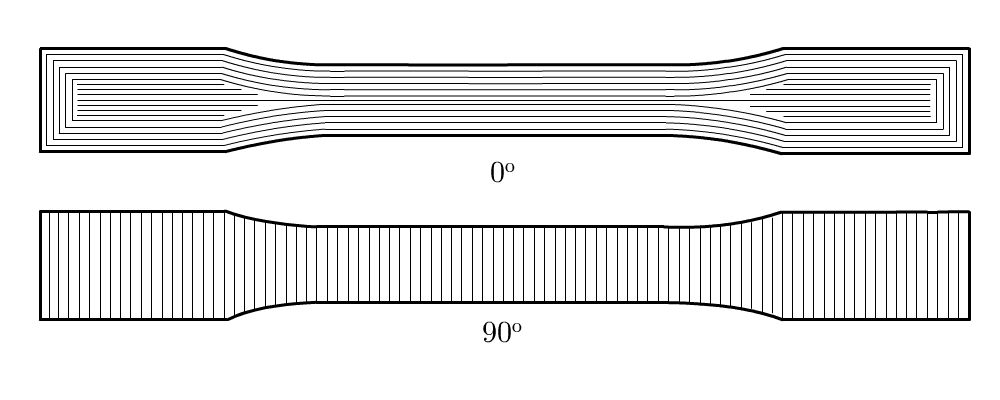
\includegraphics[width=0.7\linewidth, keepaspectratio]{090db}
	\caption{Toolpath considerations for the tensile coupons} \label{fig:090db}
\end{figure}

\subsection{Compressive Specimens}

Compressive samples were designed with a tubular cross section. This geometry was chosen to mitigate hydrostatic stresses that could artificially increase the compressive strength of the sample if it were made as a completely solid object. Additionally, the cylindrical geometry allowed production of the 0$^\circ$ samples in \emph{Otto}. The geometry can be seen in Figure \ref{fig:comp}.
\begin{figure}[h]
	\center
	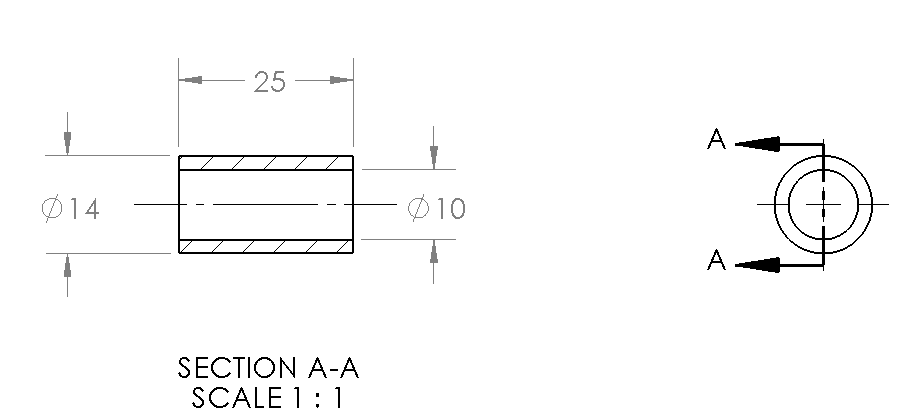
\includegraphics[height=6cm, keepaspectratio]{compres}
	\caption{Compression specimen geometry} \label{fig:comp}
\end{figure}

Compression samples with a bead orientation of 90$^\circ$ with respect to the loading direction were produced using the TAZ5 and \emph{SciSlice}. The coupons with a bead orientation of 0$^\circ$ with respect to the loading direction were made using \emph{Otto} and a customized \emph{Python} script that converted process parameters into instructions for the robotic arm through ABB's \emph{RAPID} toolpathing language. A visual representation of the specimens can be seen in Figure \ref{fig:comp_d}. 
\begin{figure}[h]
	\center
	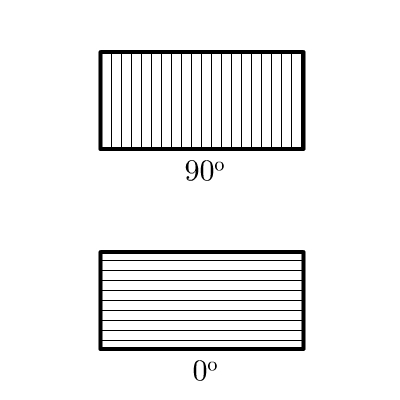
\includegraphics[height=5cm, keepaspectratio]{comp_diagram}
	\caption{Representation of compression samples} \label{fig:comp_d}
\end{figure}

\subsection{Torsion and Combined Loading Specimens}

The geometry of the torsion specimens was loosely based in the EN ISO 3167, Type A specimens used by Obst \emph{et al.} \cite{Obst2018}. The cross sectional area of the testing area was chosen to be the same as for the compression specimens. This geometry was chosen since its tubular arrangement allows easy integration with the 6-axis robotic printer, as well as offering axisymmetry and reduction of the risk of artificially increasing the strength of the sample due to yielding restrictions associated with using a completely solid coupon \cite{Obst2018}. However, due to toolpathing complications, more than one torsion geometry was necessary. Each one is described in detail below.  

\subsubsection{45$^\circ$ torsion samples}

To test the $\sigma_{11}$-$\sigma_{22}$ interaction, a torsion sample with beads oriented in 45$^\circ$ was necessary. The geometry, which can be seen in Figure \ref{fig:tors45}, consists of a specimen of cylindrical nature, with a filleted, widening change in cross sectional area that culminates in a gripping section. In this portion, three flat surfaces are added to ensure proper contact with the grips of the torsion machine. 
\begin{figure}[h]
	\center
	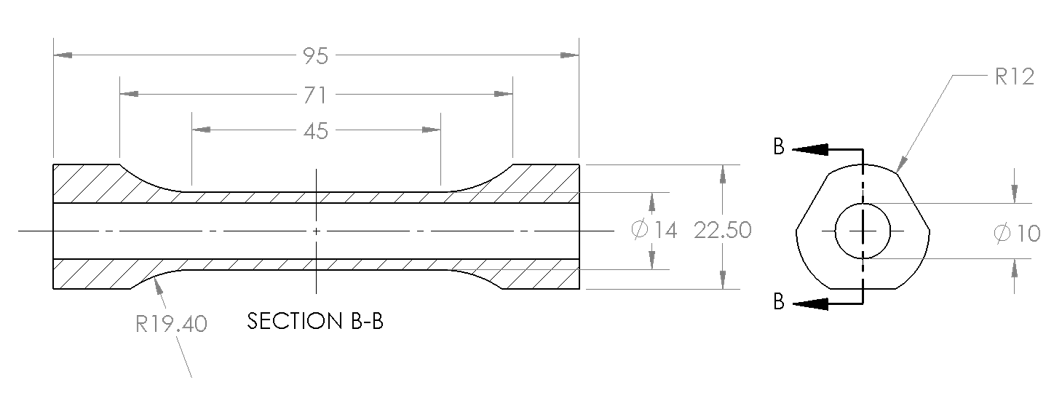
\includegraphics[width=\linewidth, keepaspectratio]{torsion}
	\caption{$S_{45}$ Torsion specimen geometry} \label{fig:tors45}
\end{figure}

The manufacturing of this type of specimen through \emph{Otto} involved laying 10 layers of beads in a 45$^\circ$ angle atop a cylindrical core of 10 mm in diameter and 95 mm in height. Finally, the gripping section is added using beads in alternating  $\pm$45$^\circ$ orientations, culminating in a wider area with a diameter of 24 mm. The flat areas had to be machined in post processing by producing cuts of 1.5 mm in depth in the grips, separated by 120$^\circ$. A visual representation of the finished sample can be seen in Figure \ref{fig:tors45d}. Note that the disposable build surface (visible on the left side of the figure) becomes a part of the coupon without impacting the gage section of the sample. All toolpath was generated using a customized  \emph{Python} script that converted process parameters into instructions for the robotic arm.
\begin{figure}[!htbp]
	\center
	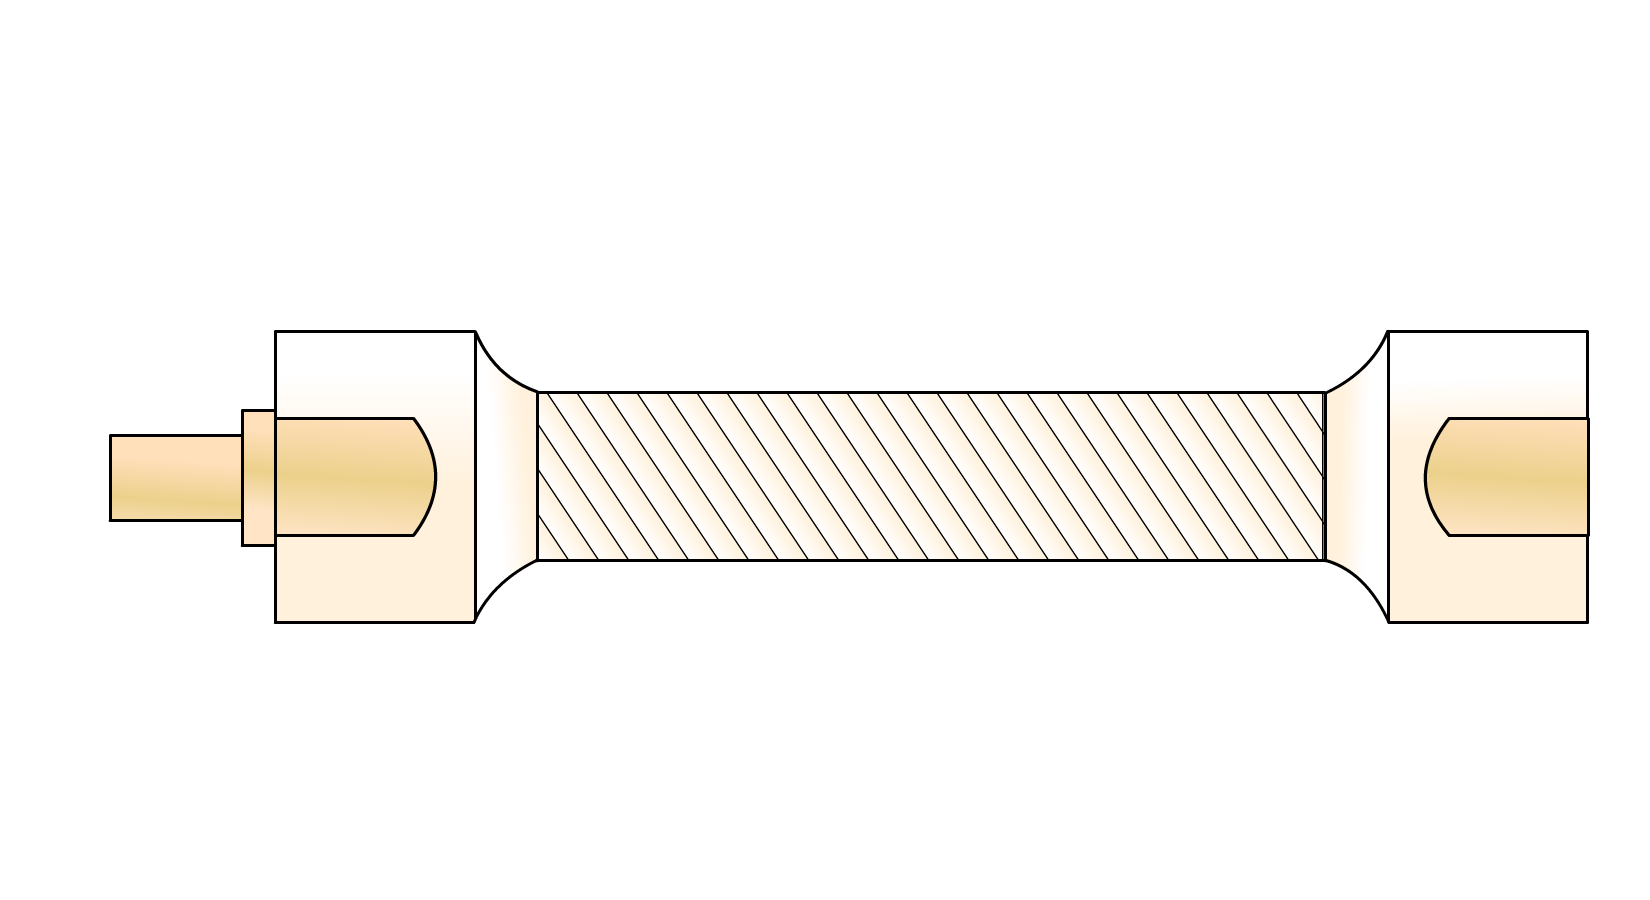
\includegraphics[width=0.35\linewidth, keepaspectratio]{Torsion_45}
	\caption{$S_{45}$ Representation of the 45$^\circ$ specimen} \label{fig:tors45d}
\end{figure}

\subsubsection{0$^\circ$ and 90$^\circ$ torsion samples}
For the 0$^\circ$ and 90$^\circ$ bead orientations, a specimen redesign was necessary due to toolpathing problems. Specifically, the length of the 45$^\circ$ torsion specimens proved problematic to print using 0$^\circ$ and 90$^\circ$ orientations, each for different reasons. In the case of the 0$^\circ$ orientation, the long and unidirectional travel distance of each bead introduced considerable tool pressure on the core, causing bowing. This was significant enough to cause poor adhesion of the beads towards the end of the specimen. By contrast, the 90$^\circ$ samples caused the sixth axis of the robot to heat up considerably and to almost completely maximize its range. 

The modified torsion sample was redesigned to have the same cross sectional area as the original 45$^\circ$ torsion samples, but shorter length. An optimal distance was devised through multiple print trials where the length of the specimen was varied between 95 and 50 mm. The final chosen geometry is shown below in Figure ????.%ELABORATE

\section{Mechanical Testing}

\subsection{Tension and Compression tests}
Tensile and compressive tests were performed with an Instron 5967 Dual Column Universal testing machine, using a 30 kN load cell. All data acquisition was handled through the accompanying Instron Bluehill 3 software. A movement speed of 5 mm/min was used to deform the 50 mm gage section of the tensile specimens, while a testing speed of 2.5 mm/min was used to deform the 25 mm of height of the compression samples. These testing speeds ensured a strain rate of 0.1 min$^{-1}$ across both specimen types.

The tensile specimens were tested using clamp grips and an extensometer. To protect the samples from excessive gripping force, emery cloth tabs were used, as described by Mazzei Capote \emph{et al}~\cite{Capote2017}. Figure \ref{fig:testsetup} shows a photograph of the setup. Compressive tests were performed using standard compression platens with the universal testing machine. 
    
\subsection{Torsion and Combined loading tests}

All torsion tests were performed using an ADMET eXpert 9618 torsion machine fitted with the MTEST Quattro controller and software suite. The machine sits on a rail system that allows the sample to deform freely during testing. The equipment has two adjustable jaws, with three contact surfaces that holds the sample in place, as shown in Figure \ref{fig:testsetup}. Of the two jaws, one rotates as controlled by a servomotor, while the other is fixed in terms of angular movement. 

\begin{figure}[h]
	\center
	\subfloat[Tensile setup \label{fig:tens}]{%
		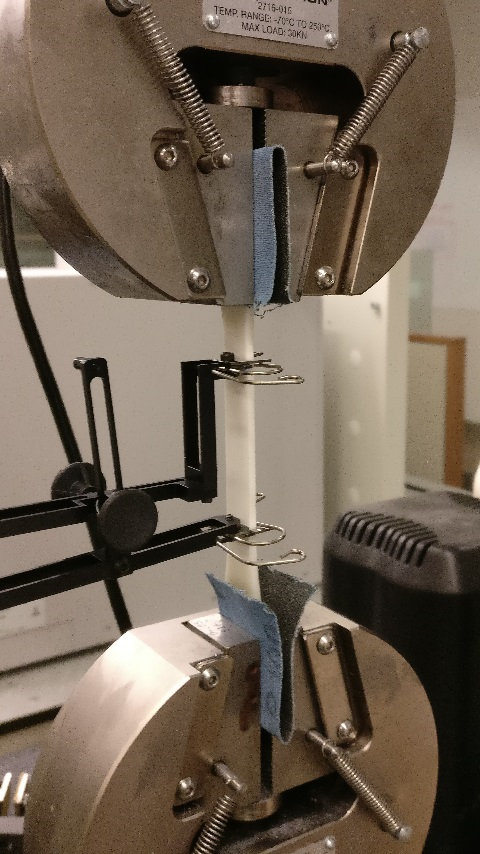
\includegraphics[height=6cm, keepaspectratio]{tensgrip}
	}
	\hfill
	\subfloat[Torsion setup\label{fig:tors}]{%
		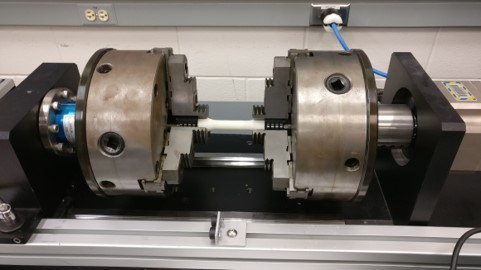
\includegraphics[height=5cm, keepaspectratio]{torsmach}
	}
	\caption{Mechanical testing setup} \label{fig:testsetup}
\end{figure} 

A conscious effort was made to maintain the same strain rate of 0.1 min$^{-1}$ used for the tensile and compression tests. The approach used was the same described by Obst \emph{et al.}~\cite{Obst2018}. The initial assumption is that the shear strain rate ($\dot{\gamma}$) is twice the engineering strain rate ($\dot{\epsilon}$), as shown in Equation \ref{eq:tors1}.

\begin{equation}\label{eq:tors1}
\dot{\gamma}= 2 \times \dot{\epsilon} 
\end{equation}

Figure \ref{fig:torscal} represents a tubular element of outer radius $\rho$ and length L, subjected to a torque T. Using this image as reference, one can see that if point B is fixed in space \textemdash as is the case of the stationary jaw of the torsion machine used throughout this work~\textemdash point A will deform to position A'. The angle of twist $\Phi$ can then be approximated using the arc length $AA'$ as $AA'=\rho \times \Phi$ for small values of shear strain~$\gamma$. It can also be seen in Figure \ref{fig:torscal} that the relationship $AA'=L\times \gamma$ also exists. From this, Equation \ref{eq:tors2} can be obtained.

\begin{figure}[h]
	\center
	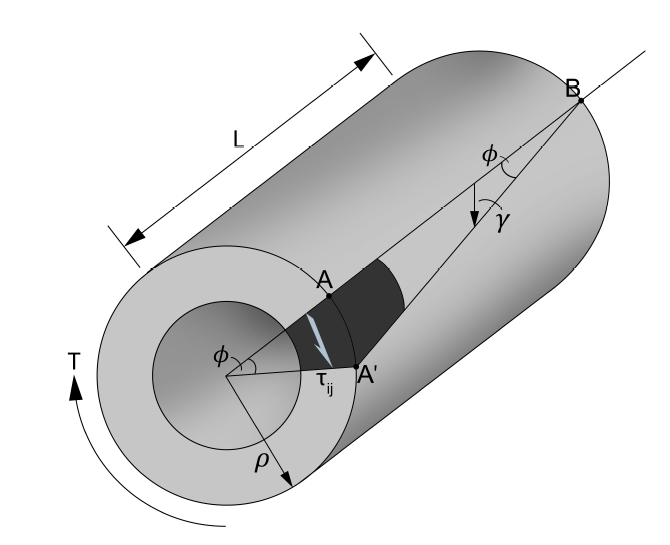
\includegraphics[width=0.55\linewidth, keepaspectratio]{tors2}
	\caption{Stress and strain caused by torque on a tubular geometry~\cite{Obst2018}} \label{fig:torscal}
\end{figure} 

\begin{equation}\label{eq:tors2}
L\times \gamma= \rho \times \Phi  
\end{equation}

Finally, after rearranging and deriving with respect to time, Equation \ref{eq:tors3} is obtained.
\begin{equation}\label{eq:tors3}
\dot{\Phi}=\frac{L\times\dot{\gamma}}{\rho}  
\end{equation}

For this work, $\dot{\gamma}$ is known to be $2 \times 0.1~min^{-1}= 0.2~min^{-1}$, as dictated by Equation \ref{eq:tors1} and the testing conditions chosen for the tensile and compressive tests. In the case of the 45$^\circ$ specimens, preliminary tests performed in positive torsion showed an average outer radius of 6.91 mm and a mean length of failure propagation of 54 mm. Using these values in Equation \ref{eq:tors3} yields a rotational speed of 1.56 rad/min, or 89.4$^\circ$/min. Following a similar procedure for the 0$^\circ$ and 90$^\circ$ samples, the angular speed of the torsion test was calculated to be ???.%ELABORATE.

\pagebreak
In the case of combined loading scenarios, the setup was fitted with a pulley system that allowed a weight to pull the sample in a nominal direction, while the torsion machine applied shear stresses. Refer to Figure \ref{fig:torscomb} for a visual representation of the compressive and tensile force setup of the torsion machine. 

\begin{figure}[!htbp]
	\center
	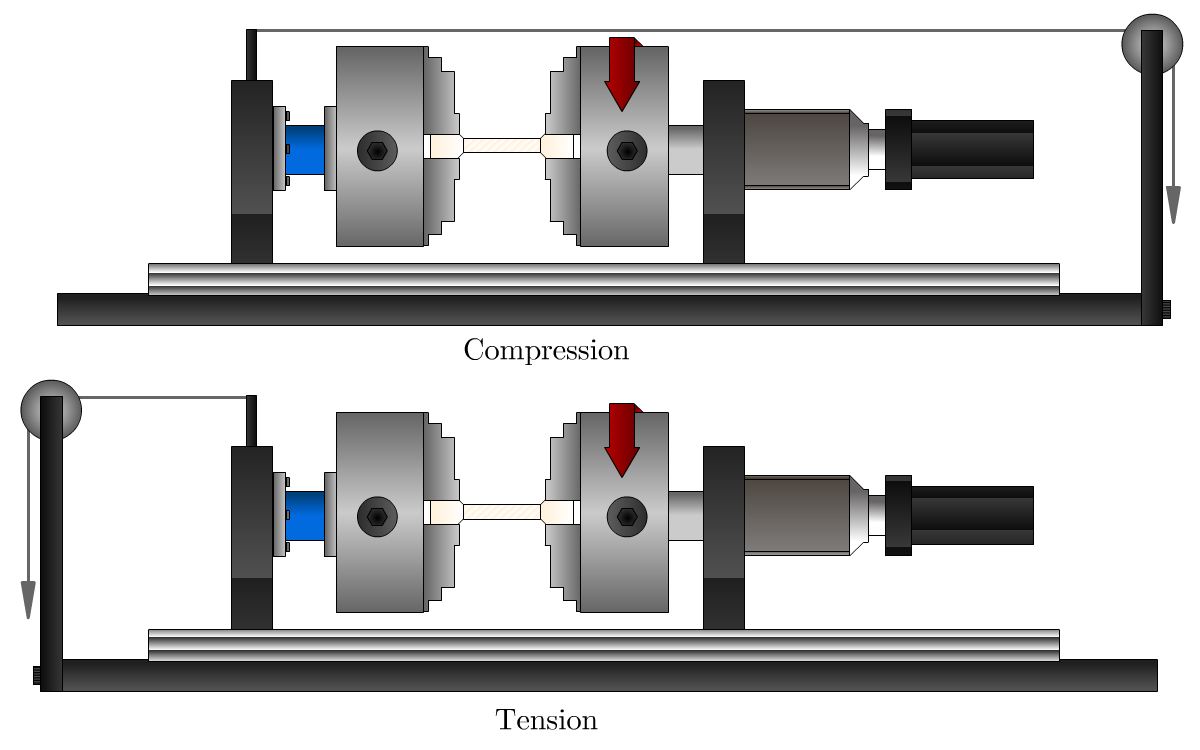
\includegraphics[width=0.8\linewidth, keepaspectratio]{torsion_machine}
	\caption{Machine setup for combined loading scenarios} \label{fig:torscomb}
\end{figure}

The shear stress from the torsion tests was obtained through Equation \ref{eq:shear}, where $\tau_{ij}$, $R$, $T$, and $J_{z}$ represent the shear stress in the $ij$\texttt{} plane, the outer radius of the test section of the sample, the Torque applied, and the second moment of area respectively.
\begin{equation}\label{eq:shear}
\tau_{ij}=\frac{T\times R}{J_{z}}  
\end{equation}

For this case, the second moment of area is defined as described in Equation \ref{eq:moment}, where $r$ represents the inner radius of the tubular specimen.

\begin{equation}\label{eq:moment}
J_{z}=\frac{\pi\times (R^4-r^4)}{2}  
\end{equation}

Finally, combining Equations \ref{eq:shear} and \ref{eq:moment}, yields Equation \ref{eq:shearf}
\begin{equation}\label{eq:shearf}
\tau_{ij}=\frac{2\times T \times R}{\pi\times(R^4-r^4)}  
\end{equation}

% Nomenclature introduced in this chapter:
\nomenclature[A]{ABS}{Acrylonitrile Butadiene Styrene}% 
\nomenclature[A]{EF}{Extrusion Factor}%

% Symbols introduced in this chapter:
\nomenclature[S]{$\epsilon$}{Engineering Strain \nomunit{$-$}}%
\nomenclature[S]{$\gamma$}{Shear Strain \nomunit{$-$}}%
\nomenclature[S]{$\dot{\epsilon}$}{Engineering Strain rate \nomunit{$min^{-1}$}}%
\nomenclature[S]{$\dot{\gamma}$}{Shear Strain rate \nomunit{$min^{-1}$}}%
\end{document}
                % results.tex
\documentclass[main.tex]{subfiles}
\begin{document}
\chapter{Results} \label{ch:res}

This chapter presents all the results originating from the experimental procedures described in Chapter \ref{ch:exp}. Additionally, details are provided regarding data processing, and the calculations that lead to the definition of the desired failure surface. 

\section{Tensile Tests} \label{sec:tensr}
Performing tensile tests showed that the values of $X_t$ and $Y_t$ were significantly different, in accordance to the literature review presented in Section \ref{ssec:mechPropFFF}. An initial number of 20 samples per orientation was produced, however, multiple specimens failed outside the gage section of the coupon and thus, data originating from these coupons was considered invalid and promptly discarded. The valid results are summarized in Table \ref{tab:tensrtab}. Note that $X_t$ was on average 9.16 MPa higher than $Y_t$, a difference of 22.7\%.
\begin{table} [h]
	\centering
	\caption{Summary of Tensile tests}
\begin{tabular}{ c| c c } 
	\toprule
	\textbf{Information} & $X_t$ & $Y_t$\\
	\midrule
	Average [MPa] & 40.29 & 31.13\\
	Standard Deviation & 0.75 & 0.58\\
	Number of samples & 19 & 12\\
	Lowest measurement [MPa] &39.37  & 29.68\\
	Highest measurement [MPa] &40.90 & 32.08\\
	\bottomrule
\end{tabular}
\label{tab:tensrtab}
\end{table}

The behavior of both sets of samples was completely different. Coupons used to measure $X_t$ clearly showed whitening of the gage section, indicating plastic deformation. Specimens used for $Y_t$ on the other hand generally failed between beads and rarely showed any change in color. Figure~\ref{fig:tensComp} clearly shows the difference in mechanical behavior. Note how the $X_t$ specimen shows a ductile failure, as opposed to brittle breakage for the $Y_t$ sample. Figure \ref{fig:tensSComp} shows both tested samples side by side.
\pagebreak

\begin{figure}[h]
	\center
	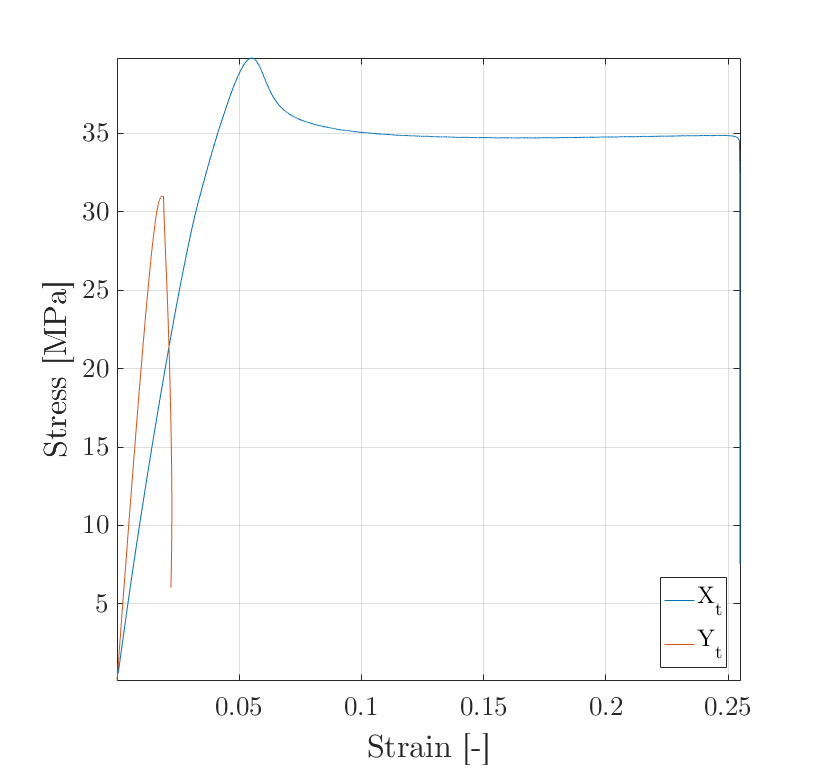
\includegraphics[height=9cm, keepaspectratio]{tenscomp}
	\caption{Comparison of tensile results} \label{fig:tensComp}
\end{figure}

\begin{figure}[!htbp]
	\center
	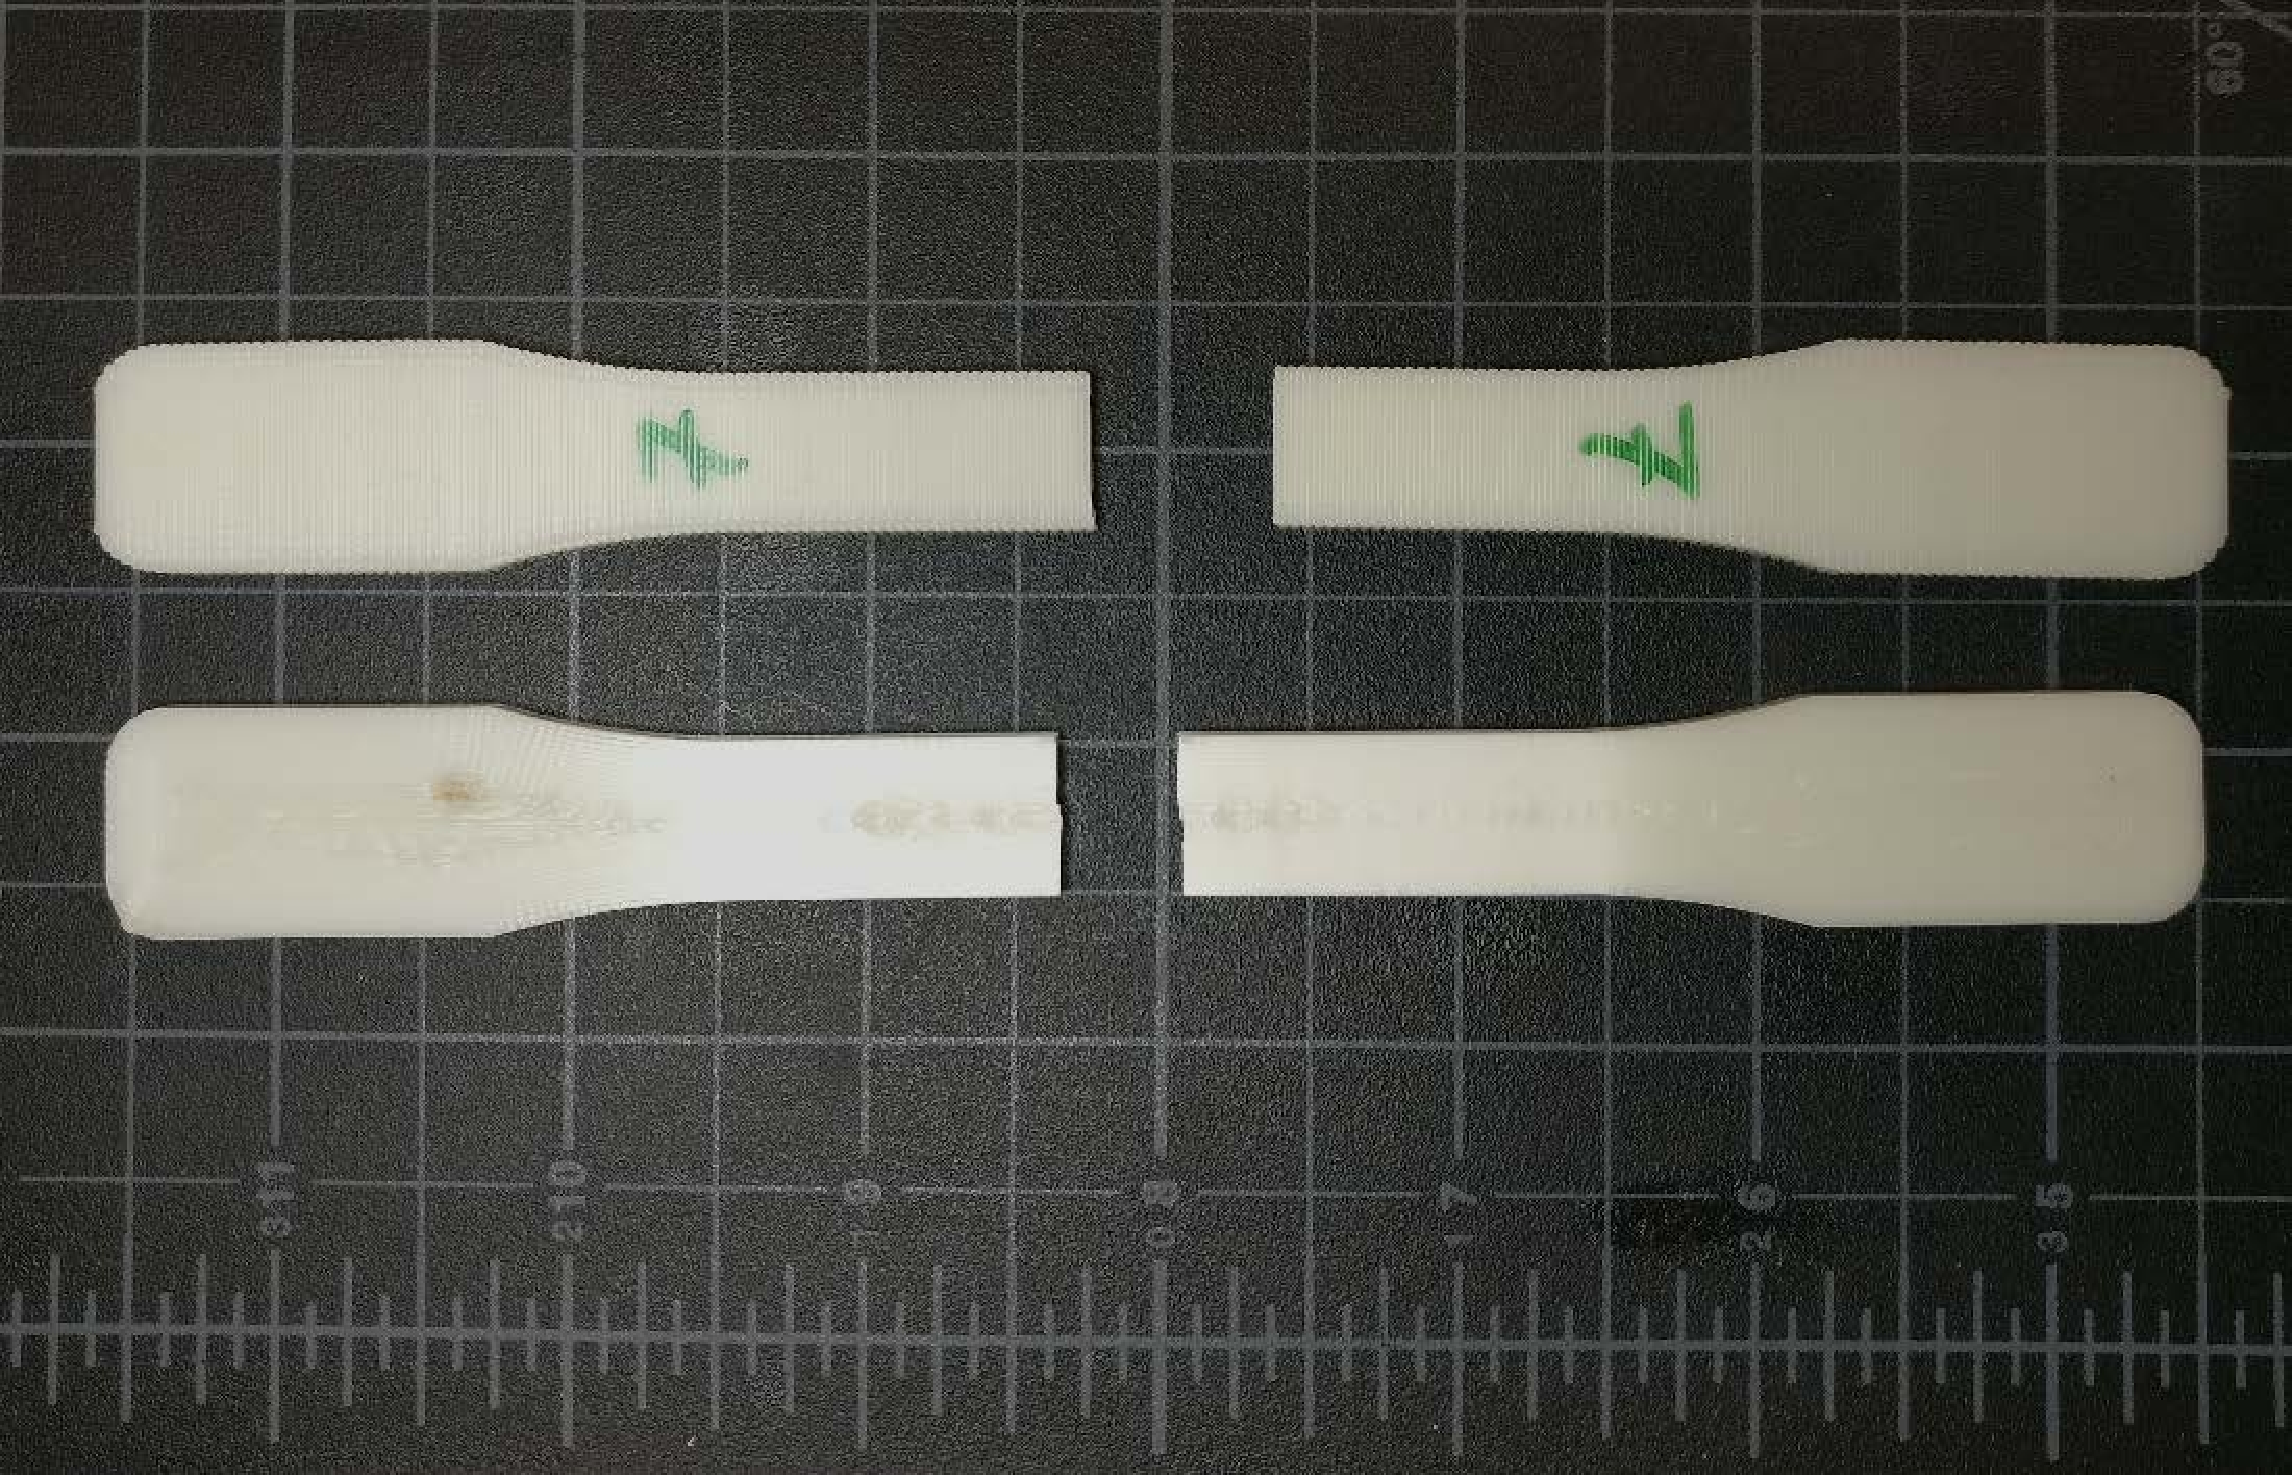
\includegraphics[height=6cm, keepaspectratio]{tenscsomp.pdf}
	\captionsetup{justification=centering} %long caption
	\caption[$X_t$ and $Y_t$ tested samples]{$Y_t$ (top) and $X_t$ (bottom) tested samples. Scale in inches. Note whitening in gage section for $X_t$ specimen.} \label{fig:tensSComp}
\end{figure}

Anderson-Darling tests (ADT) were performed on the results to validate if the data follows a normalized distribution. In the case of $X_t$, the ADT yields a p-value of 0.023. Thus, on a 95\% confidence interval, a normalized distribution can be discarded. This can be seen graphically in the goodness of fit plot, where data points fail to align with the slope that corresponds to a theoretical Gaussian distribution. By contrast, performing the ADT on the $Y_t$ samples fails to reject a normalized distribution using the same confidence interval, offering a p-value of 0.109. %A case could be made for a false negative for $X_t$ and a false positive for $Y_t$, given the relatively small sample size for each data set.
The results from ADT can be seen in Figure \ref{fig:adttens}.

%FIX
\begin{figure}[!htbp]
	\center
	\subfloat[$X_t$ \label{fig:adtxt}]{%
		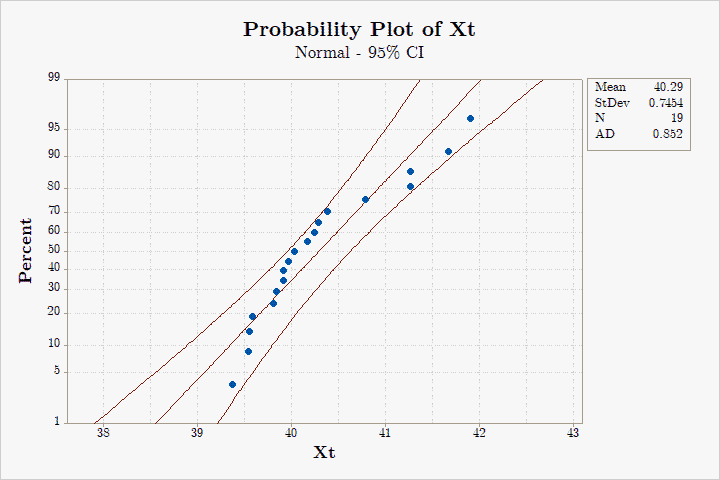
\includegraphics[height=8.5cm, keepaspectratio]{PP_Xt}
	}
	\hfill
	\subfloat[$Y_t$\label{fig:adtyt}]{%
		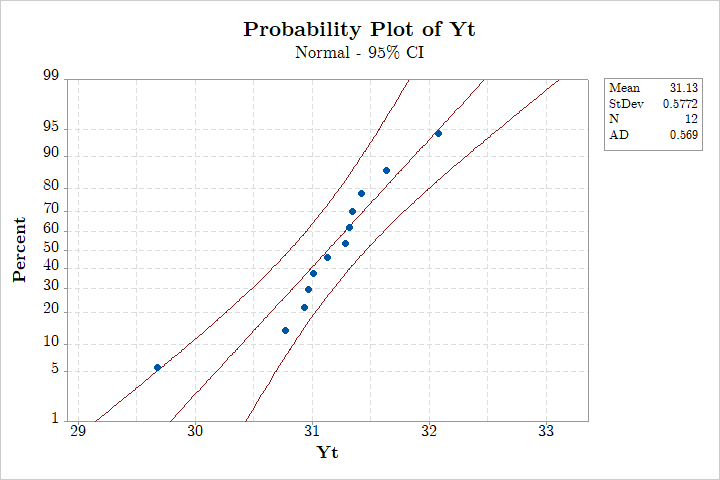
\includegraphics[height=8.5cm, keepaspectratio]{PP_Yt}
	}
	\caption{ADT results for tensile data} \label{fig:adttens}
\end{figure}

\pagebreak
      
\section{Compression Tests} \label{sec:compr}
For the compression tests, a total of 25 samples were produced for each orientation. However, a number of coupons were discarded due to manufacturing defects. Table \ref{tab:comprtab} summarizes the test results.  

\begin{table} [h]
	\centering
	\caption{Summary of Compression tests}%ELABORATE
	\begin{tabular}{ c| c c } 
		\toprule
		\textbf{Information} & $X_c$ & $Y_c$\\
		\midrule
		Average [MPa] &43.91  & 57.96\\
		Standard Deviation &3.23  & 1.81\\
		Number of samples &25  & 22\\
		Lowest measurement [MPa] &37.95 &54.93 \\
		Highest measurement [MPa] &48.87 &61.39 \\
		\bottomrule
	\end{tabular}
\label{tab:comprtab}
\end{table}

Surprisingly, both sets of specimens had different failure behavior. The $Y_c$ samples displayed pure ductile behavior through testing. A clear maximum stress can be observed at the yield point in a stress-strain graph, and all samples showed localized whitening and deformation along the center of the specimen. By contrast, the $X_c$ samples showed a considerably lower yield point, cracking sounds were common during testing, and specimens deformed in a way that formed petal-like structures due to contiguous bead delamination. Figure \ref{fig:CompSComp} shows $X_c$ and $Y_c$ samples side by side post testing, where the different failure behavior becomes evident.

\begin{figure}[!htbp]
	\center
	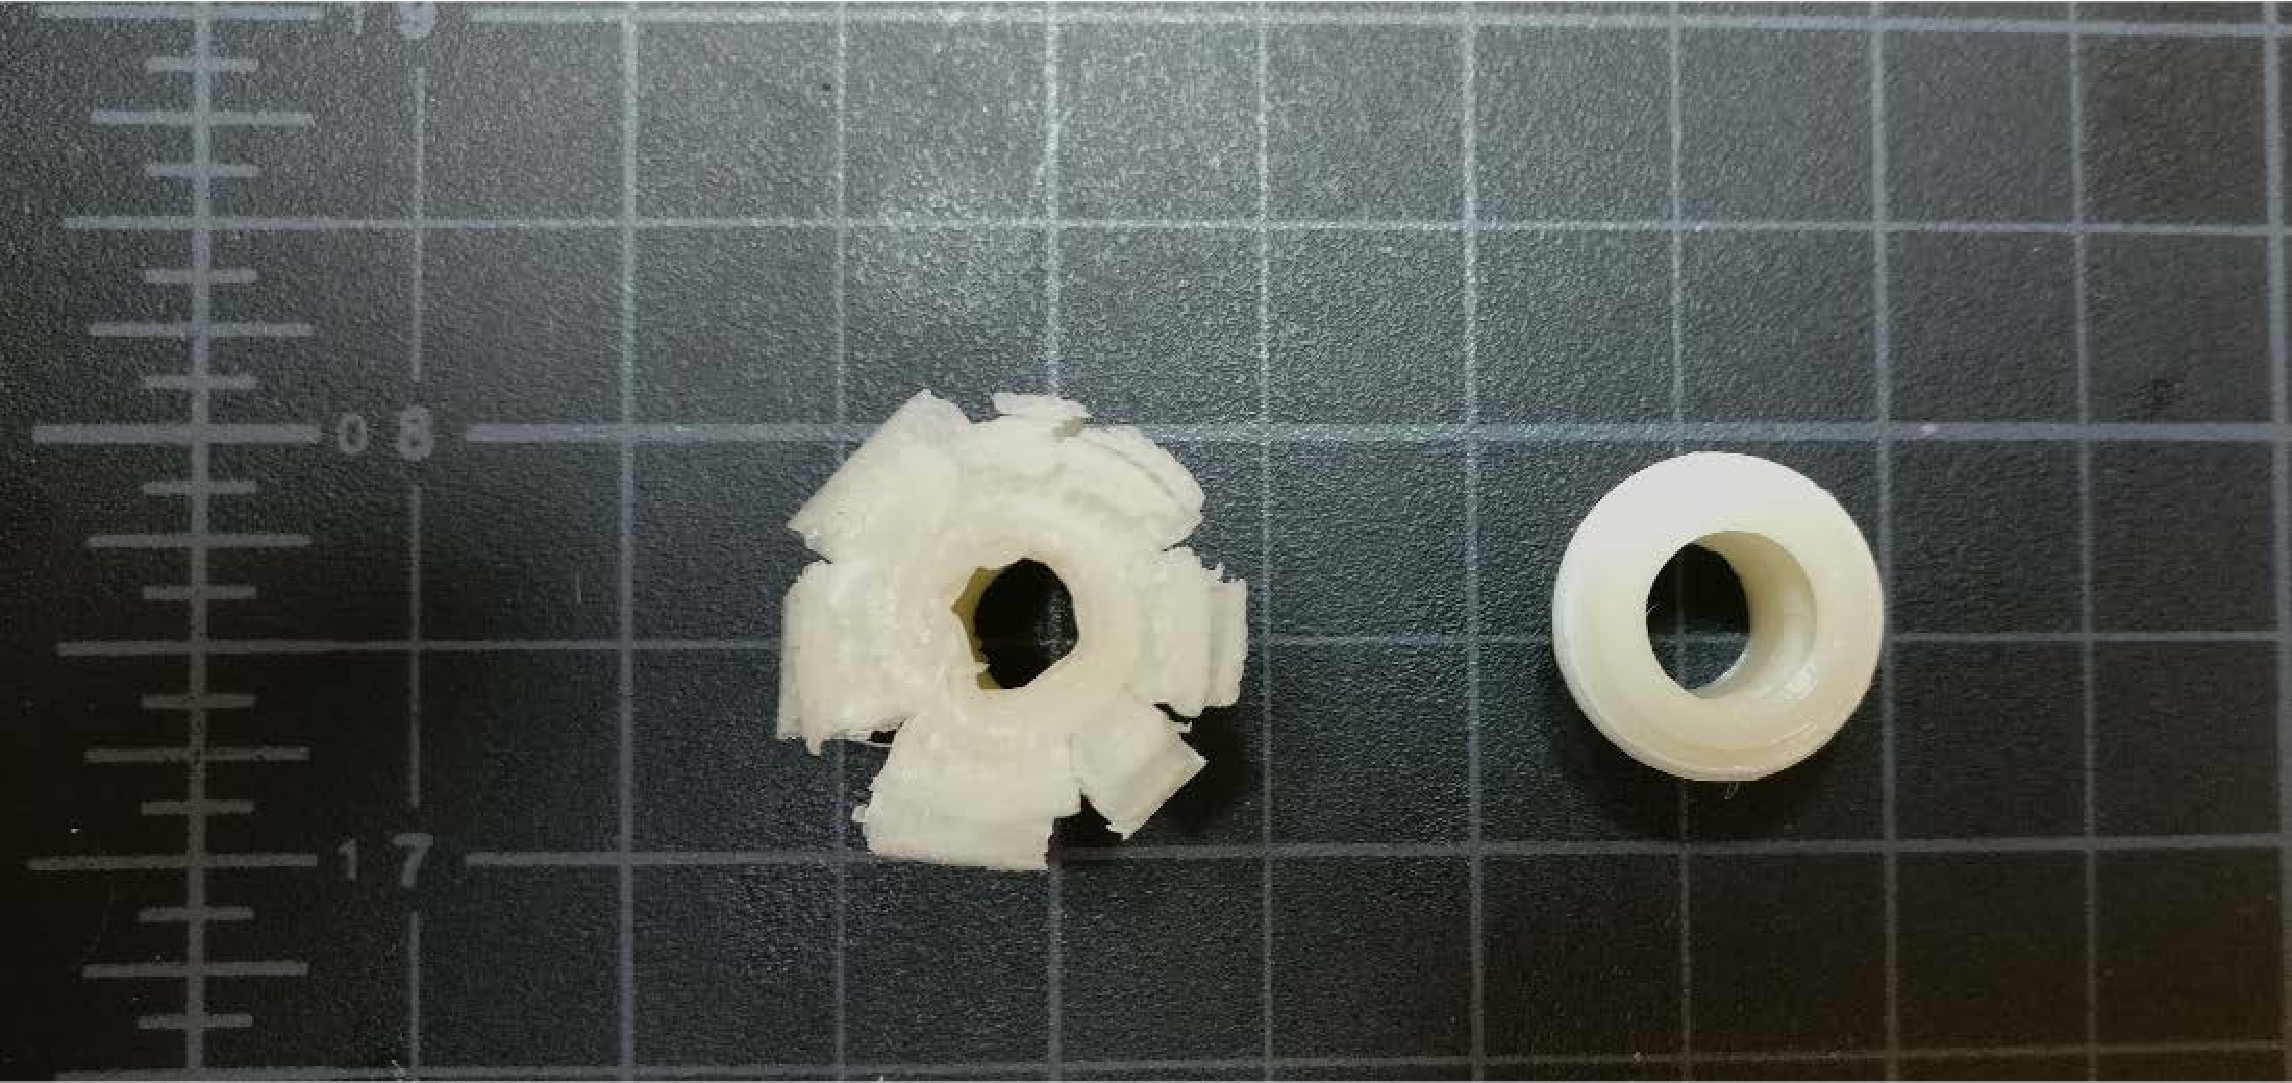
\includegraphics[height=6cm, keepaspectratio]{compscomp.pdf}
	\captionsetup{justification=centering} %long caption
	\caption[$X_c$ and $Y_c$ tested samples]{$X_c$ (left) and $Y_c$ (right) tested samples. Scale in inches. Note petal-like structure of $X_c$ sample.} \label{fig:CompSComp}
\end{figure}

The difference in mechanical behavior can be seen clearly in Figure \ref{fig:comprComp}, where stress-strain curves for $X_c$ and $Y_c$ are compared. Note the erratic behavior of the $X_c$ sample, caused by delamination of adjacent beads.  

\begin{figure}[!htbp]
	\center
	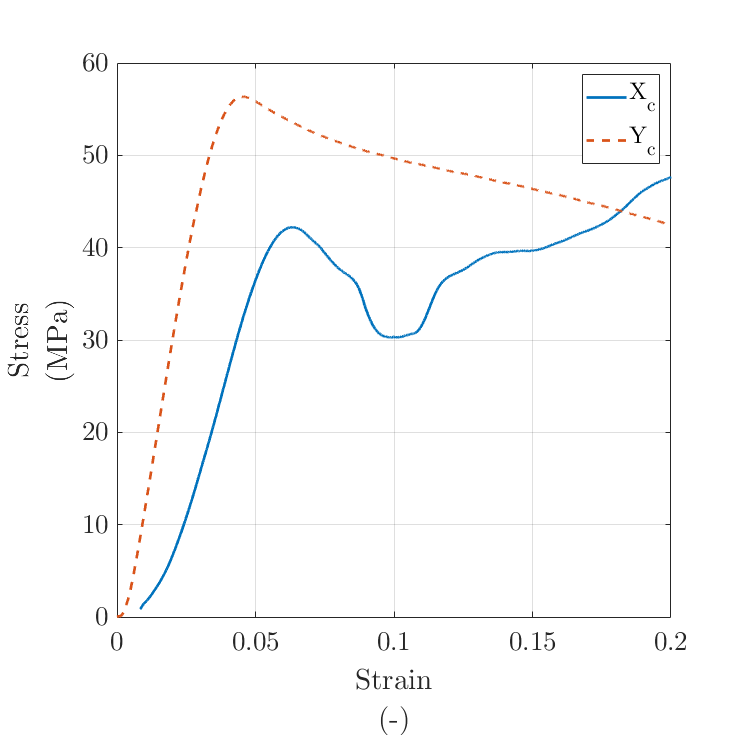
\includegraphics[height=9cm, keepaspectratio]{compresscomp}
	\caption{Comparison of compression results} \label{fig:comprComp}
\end{figure}  

Performing ADT on the data reveals a p-value of 0.072 for $Y_c$, and 0.056 for $X_c$, thus, normalized distributions cannot be discarded on a 95\% confidence interval. These tests can be seen in Figure \ref{fig:adtcomp}. %ELABORATE

\begin{figure}[!htbp]
	\center
	\subfloat[$X_c$ \label{fig:adtxc}]{%
		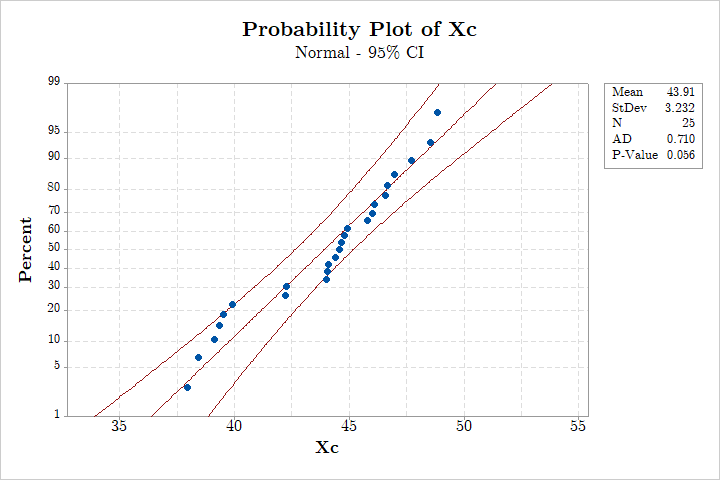
\includegraphics[height=8.5cm, keepaspectratio]{PP_Xc}
	}
	\hfill
	\subfloat[$Y_c$\label{fig:adtyc}]{
		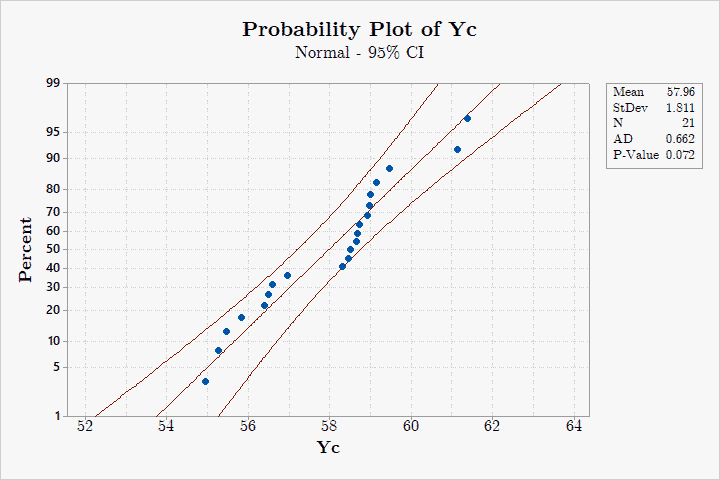
\includegraphics[height=8.5cm, keepaspectratio]{PP_Yc}
	}
	\caption{ADT results for compression tests} \label{fig:adtcomp}
\end{figure}

\section{Torsion Tests} \label{sec:torsr}
\subsection{45$^\circ$ orientation} \label{ssec:45r}
A total of 30 samples were produced with a 45$^\circ$ bead orientation, divided evenly for tests in positive and negative shear. As was the case for tensile and compressive tests, a number of specimens had to be discarded due to undesired behavior during testing. A common problem was delamination of the grips, thus requiring the data to be discarded. 

Results showed significant difference in behavior depending on the direction of the applied torque. The $S_{45p}$ samples showed a completely brittle behavior, with fracture occurring between beads, as opposed to ductile failure in the center of the specimen for the $S_{45n}$ coupons. This resulted in an average difference of 6.3 MPa between both sets of data. Results are summarized in Table \ref{tab:tors45r} and a graph comparing the behavior of both sets of samples can be seen in Figure \ref{fig:45comp}. Note how the positive shear sample fails at low angles in a completely brittle manner.

\begin{table} [h]
	\centering
	\caption{Summary of 45$^\circ$ torsion tests}
\begin{tabular}{ c| c c } 
	\toprule
	\textbf{Information} & $S_{45p}$ & $S_{45n}$\\
	\midrule
	Average [MPa] & 20.80 & 27.13\\
	Standard Deviation & 2.50 & 0.50\\
	Number of samples & 9 & 9\\
	Lowest measurement [MPa] &17.21  & 26.59\\
	Highest measurement [MPa] &24.61 & 28.17\\
	\bottomrule
\end{tabular}
\label{tab:tors45r}
\end{table}

\begin{figure}[!htbp]
	\center
	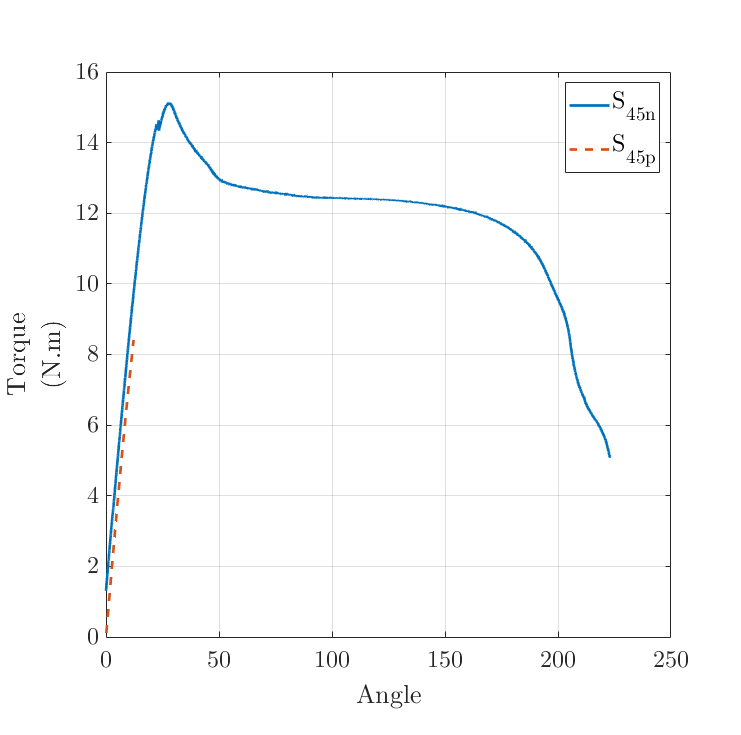
\includegraphics[height=9cm, keepaspectratio]{comp45t}
	\caption{Comparison of 45$^\circ$ torsion results} \label{fig:45comp}
\end{figure}

\begin{figure}[!htbp]
	\center
	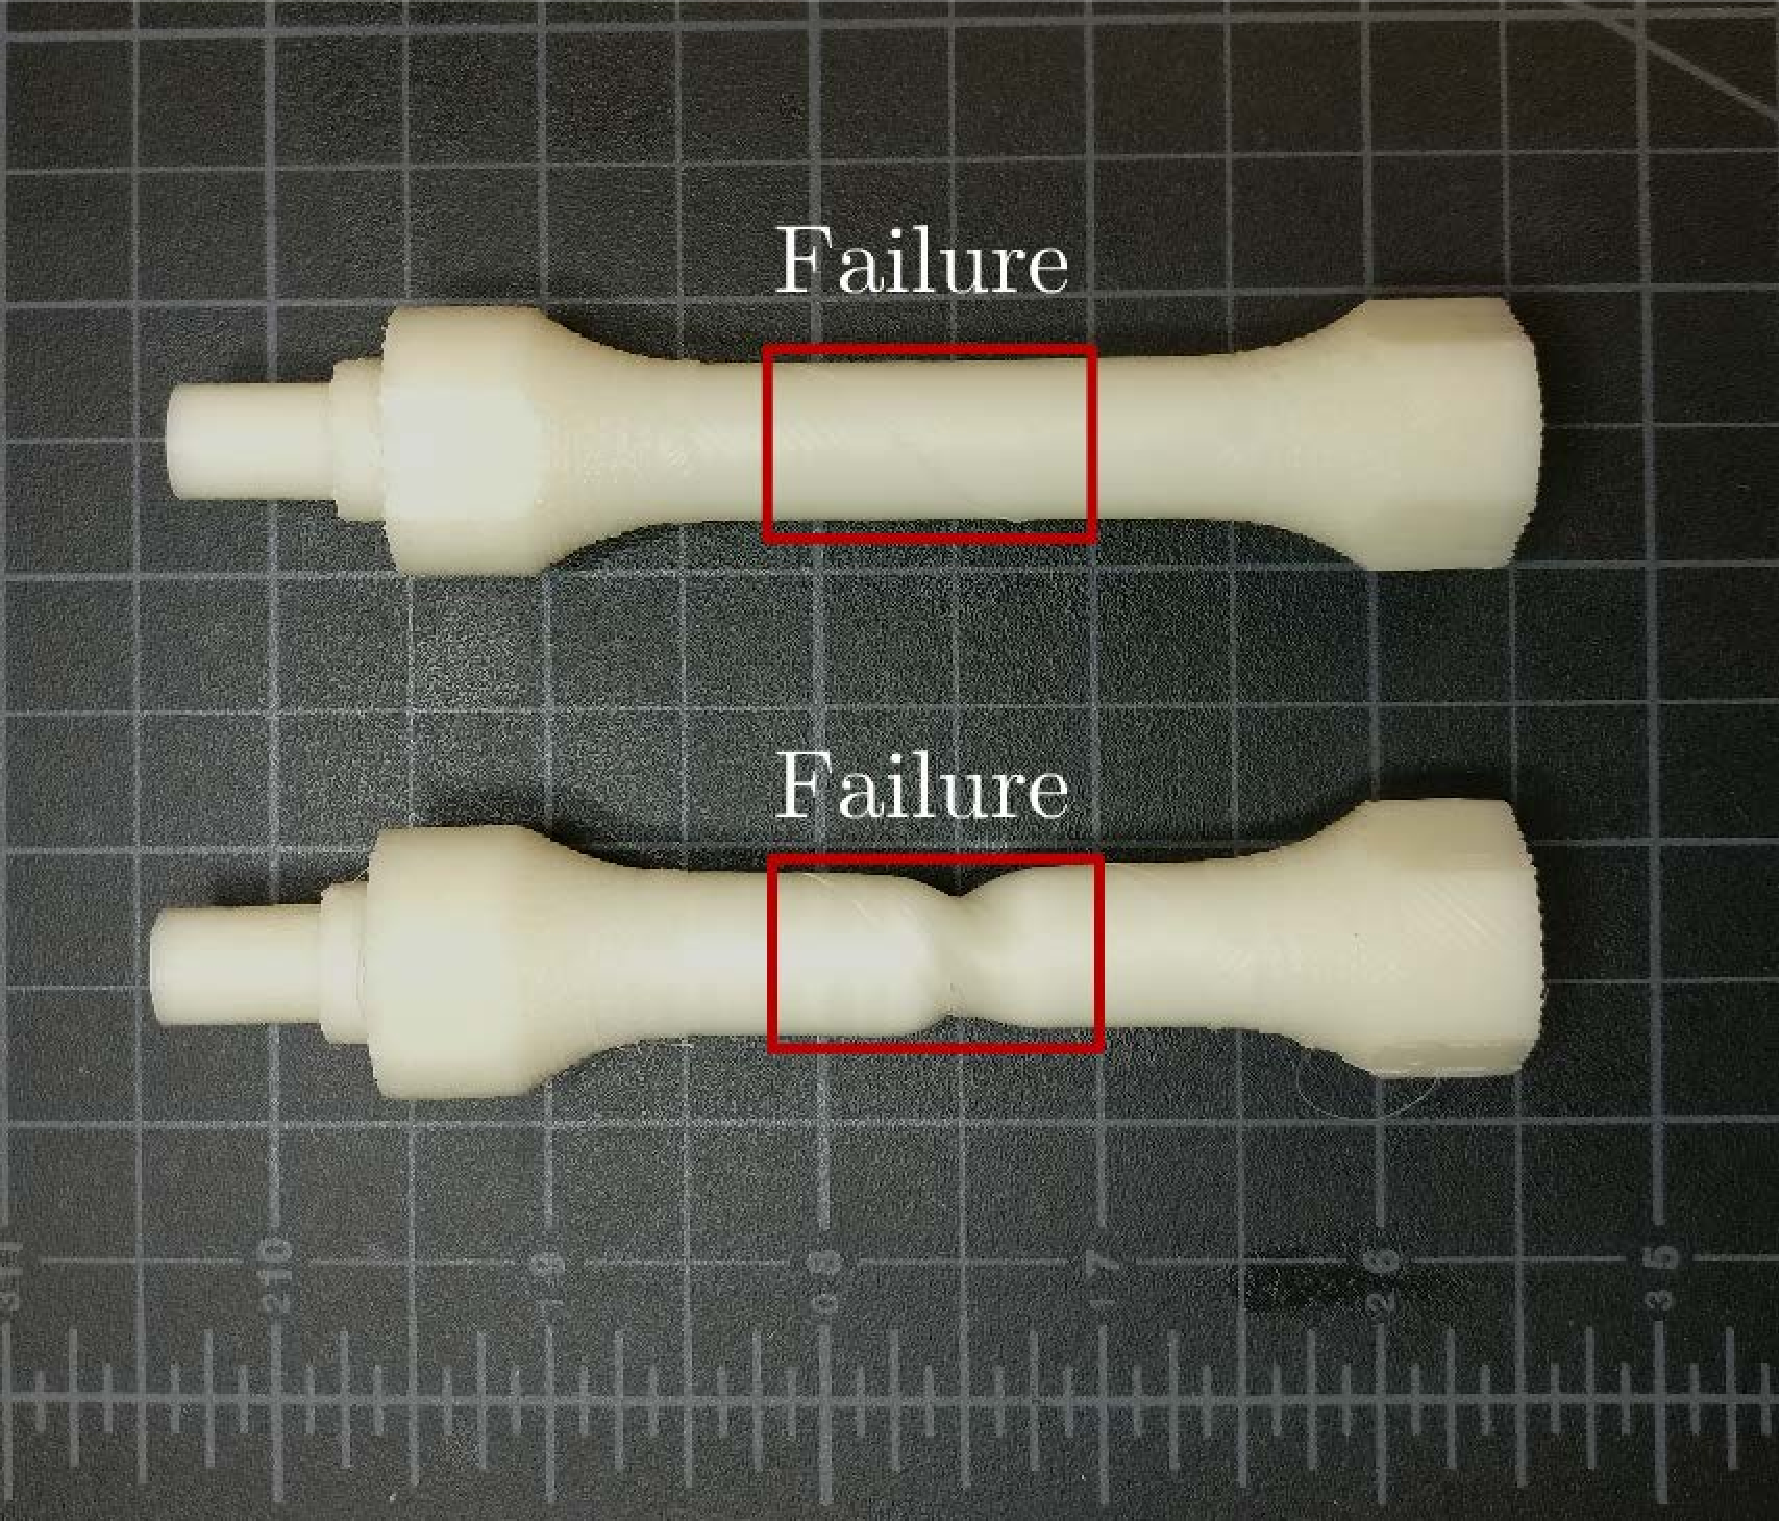
\includegraphics[height=7cm, keepaspectratio]{t45scomp}
	\captionsetup{justification=centering} %long caption
	\caption[Comparison of 45$^\circ$ torsion results]{Comparison of 45$^\circ$ torsion samples. Positive shear (top) caused bead delamination and brittle failure, whereas negative shear (bottom) produced plastic deformation of the gage section} \label{fig:45scomp}
\end{figure}
  
\subsection{0$^\circ$ and 90$^\circ$ orientation} \label{ssec:090r}

A total of 10 samples was produced for each orientation. Table \ref{tab:tors090r} summarizes the results from the torsion tests.

\begin{table} [h]
	\centering
	\caption{Summary of 0$^\circ$ and 90$^\circ$ torsion tests}
\begin{tabular}{ c| c c } 
	\toprule
	\textbf{Information} & $S_{0}$ & $S_{90}$\\
	\midrule
	Average [MPa] &  & \\
	Standard Deviation & & \\
	Number of samples &  & \\
	Lowest measurement [MPa] &  & \\
	Highest measurement [MPa] & & \\
	\bottomrule
\end{tabular}
\label{tab:tors090r}
\end{table}

\section{Combined Loading Tests} \label{sec:clr}

The combined loading scenarios involved testing 10 samples in shear and tension, and 10 for shear and compression, totaling 20 samples for each orientation. 
 
\section{Development of the Failure Surface} \label{sec:fsc}

The failure surface calculations were performed using MATLAB\textregistered~code based on previous work by Obst \emph{et al.} \cite{Obst2018} and the mathematical relations shown in Chapter \ref{ch:oocrit}. This code can be found in Appendix \ref{ch:fsurfcode} for reference.

Calculations were based on the average values obtained from the mechanical tests in order to incorporate a probabilistic approach as developed by Zaitsev, Pashkov and Strelyaev \cite{Zaitsev1975}. In practice, this signifies that the condition $f=1$ in Equation \ref{eq:GKCfinal} is equivalent to a probability of part failure equal to 50\%.

Starting with the $\sigma_{11}$-$\sigma_{22}$ plane, it can be seen that the failure envelope has a notable tilt, agreeing with the difference observed between compressive and tensile strengths in both directions, as well as the difference in behavior for the $S_{45}$ tests. Refer to Figure \ref{fig:1122plane} for a graph showing the calculated failure envelope, including the experimental data for reference.

\begin{figure}[!htbp]
	\center
	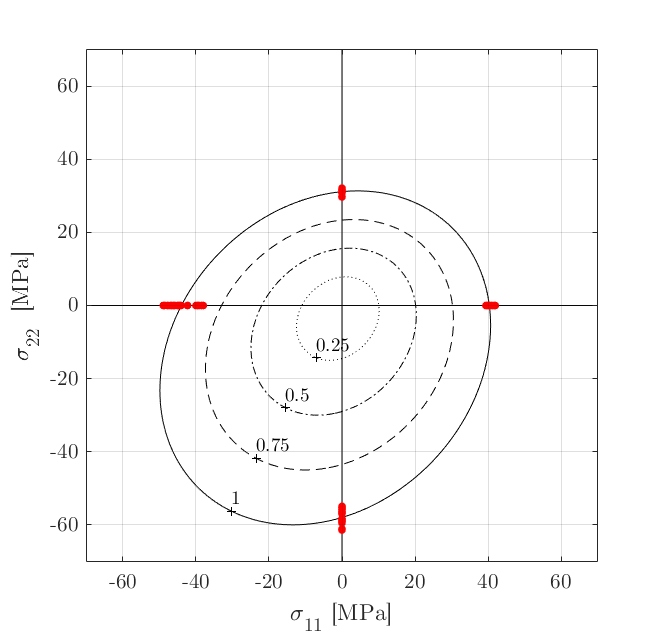
\includegraphics[width=\linewidth, keepaspectratio]{11_22plane}
	\captionsetup{justification=centering} %long caption
	\caption[failure envelope in the $\sigma_{11}$-$\sigma_{22}$ plane]{$\sigma_{11}$-$\sigma_{22}$ plane including data of $X_t$, $X_c$, $Y_t$ and $Y_c$ tests. Graph shows calculated f values of 1, 0.75, 0.50 and 0.25 to illustrate safety factors of 1, 4/3, 2 and 4 respectively} \label{fig:1122plane}
\end{figure}

It can be seen from the tilt of the envelope that there's a strong interaction between the transverse and longitudinal stresses. Computing all tensorial components associated with the  $\sigma_{11}$-$\sigma_{22}$ plane results in Table \ref{tab:1122calc}. Note how $F_{1122}$ is negative and in the same order of magnitude as $F_{1111}$ and $F_{2222}$. 

\begin{table} [h]
	\centering
	\caption{Tensorial components obtained from tests in the $\sigma_{11}$-$\sigma_{22}$ plane}
	\begin{tabular}{ c c } 
		\toprule
		\textbf{Component} & \textbf{Value} \\
		\midrule
		$F_{11}$ & 1.023$\times 10^{-3}$\\ [1ex]
		$F_{1111}$ & 5.663$\times 10^{-4}$\\ [1ex]
		$F_{22}$ & 7.435$\times 10^{-3}$\\ [1ex]
		$F_{2222}$ & 6.095$\times 10^{-4}$\\ [1ex]
		$F_{1122}$ & -3.139$\times 10^{-4}$\\ [1ex]
		\bottomrule
	\end{tabular}
	\label{tab:1122calc}
\end{table}  

Figure \ref{fig:1122plane} indicates that FFF parts produced with the print parameters used should show considerable strengthening when loaded bi-axially in compression. Further experimental work would be of interest to compare bi-axial compression test data to this result.


% Nomenclature introduced in this chapter:
\nomenclature[A]{ADT}{Anderson-Darling Test}% 

% Symbols introduced in this chapter:
%\nomenclature[S]{$\epsilon$}{Engineering Strain \nomunit{$-$}}%
\end{document}
                %% toolpath.tex

\documentclass[main.tex]{subfiles}
\begin{document}

\chapter{Robot Programming}
Two options are commonly available for programming most industrial robots: produce a standard G-code program and run it through the robot's G-code interpreter or use the robot's native programming language.
Using G-code is useful when the robot's tool paths will be generated by standard computer aided manufacturing (CAM) software packages.
\nomenclature[A]{CAM}{Computer Aided Manufacturing}
Most facilities with CNC machines already have access to CAM software and knowledgeable operators making it easy to transition from programming CNC machines to programming a robot.
CAM packages are also essential when tool paths require thousands to hundreds of thousands of points for complex machining or polishing applications.
There are, however, some disadvantages associated with using G-code on a robot.
The first disadvantage with G-code is that since it was originally designed for operating three axis CNC machines and only later expanded to handle more axes, it does not provide as rich of a command set for operating a robot as the robot's native language.
This can limit a programmer's ability to access robot specific reposition commands, handle advanced motion planning tasks, or interface with external devices.

A second disadvantage lies in needing to know the implementation and reliability of the robot's G-code interpreter.
Knowing which G-codes are implemented is usually simple but understanding the subtle differences which can occur between implementations can be difficult.
How will the robot move when G-code commands cause it to move near a singularity or require a different robot configuration to prevent a crash?
While these problems can also occur when using the robot's native language they become more opaque and difficult to predict with an additional layer of abstraction between the operator/programmer and the actual robot motions.

Due to the limitations present in using G-code to program the robot it was decided to use ABB's proprietary RAPID programming language for operating the robot.
By using the RAPID language it is possible to directly control the quaternions and robot configuration parameters for each point along a path making it easier to command off-axis work.
Communication between the robot and RAMBo board is easier with RAPID plus the RobotStudio environment simplifies program debugging.
For 2.5D printing it was possible to modify SciSlice to output RAPID programs instead of G-code enabling easy initial testing of the system.
When off-axis tool paths were required additional Python scripts were developed to produce the desired robot code.

When creating RAPID programs the most essential elements for making the robot move as desired are tool and work objects, motion commands, and the desired movement points.
The tool and work objects, sec. \ref{sec:toolworkobjects}, tell the robot where the tool and build platform are located providing a reference frame for the coordinate system.
Motions commands, sec. \ref{sec:motioncommands}, define how the robot should move between programmed points, i.e. straight line, arc, joint etc..
While points, or \texttt{robTarget}s, sec. \ref{sec:points}, define where the robot should move, what posture the tool should be in, and the desired robot configuration.
With these three basic items and knowledge of the robot's syntax, it is possible to create off-axis programs for the robot.



\section{Tool and Work Objects}
\label{sec:toolworkobjects}
As is done in CNC machine programming, tool and work offsets can and should be used when programming robots.
In ABB's RAPID programming language these offsets are stored in variable objects of types \texttt{tooldata} and \texttt{wobjdata}, respectively.
Unlike in CNC operations, the RAPID programming language allows a user to declare whether the robot is holding the tool or the work object.
Most applications use a robot held tool with a fixed work object but for this application it was decided to use a robot held work object (build platform) and a fixed tool (print head).
By using a robot held work object the $xyz$ coordinates used for commanding program positions become fixed to the part enabling the robot to track their locations as the part is rotated.
Calculating where the part is in space as the robot rotates, called the forward kinematics, is not overly complicated but it is work best completed by the robot itself.
With this setup a point on the part is always the same $xyz$ coordinates independent of the part's angle relative to the nozzle.
Commanding the robot to be at the same point with different orientations is done by using the same $xyz$ values and only changing the \texttt{robTarget}'s quaternion.
This makes it easy for the operator to know where on the part the robot is moving and which locations will have different orientations.
If a robot held tool and fixed work object had been used different positions around the part could be commanded with the same $xyz$ values but different quaternions, a situation deemed very difficult to read and troubleshoot.

Using tool and work objects also enables the operator to make adjustments to the tool path without editing and reloading the entire program.
If the operator notices that a new build platform was causing the initial layers of a part to be printed too high they could go into the work object representing the build platform and adjust it, fixing the tool path problem without changing the program.
It should be noted that in this situation the changing of the build platform made it obvious as to which object, tool or work, was causing the problem.
In other situations the adjustment required may not be so clear and special care should be taken when adjusting the location of the nozzle.
An adjustment in $z$\nobreakdash-height of the nozzle may fix a problem in the $xy$\nobreakdash-plane but create a new one when the work piece is rotated into a new orientation.

\subsection{Measuring the Nozzle}
As mentioned in section \ref{sec:challangenozzle}, accurately measuring the location of the nozzle in $xyz$ is critical to the quality of off-axis printed parts.
To measure the nozzle's location a 3-axis analog indicator made by Haimer, their Universal 3D-Sensor, was used which is accurate to \SI{10}{\micro m}.
A custom adapter was designed and then machined out of aluminum to attach the  3D-sensor to the robot, Fig.~\ref{fig:3Dsensor}.

\begin{figure}
\centering
	\begin{overpic}[width=0.8\textwidth, keepaspectratio]
		{3DSensor.pdf}
		\put(70,43){Robot Arm}
		\put(45,35){Adapter}
		\put(43,1.5){3D Sensor}
		\put(15,12){\makebox(0,0)[r]{Stylus on nozzle}}
	\end{overpic}
	\caption{Haimer 3D Sensor measuring nozzle location.}
	\label{fig:3Dsensor}
\end{figure}

\subsubsection{3D-Sensor Calibration}
Before making accurate measurements with the 3D-sensor the run-out of the tool must be minimized and the gauge length needs to be properly calibrated.
Run-out is minimized by adjusting the four run-out screws on the sensor and checked by rotating the sixth axis while the stylus is contacting a dial indicator.
With patience a run-out of less than \SI{2}{\micro m} can be achieved.

The gauge length of the sensor is measured from the mounting face of the sixth axis to the position of the stylus's tip when the dial reads zero in the $z$ direction.
To calibrate this value a reference location with a known $z$\nobreakdash-height must be developed.
This reference location was developed by commanding the sixth axis to be parallel with the safety enclosure's table and then driving the robot until a gauge block just fit between the table and the sixth axis's face.
From here the robot's $z$\nobreakdash-height is checked and by accounting for the height of the gauge block the $z$\nobreakdash-height of the reference position is known.
After the sensor is mounted on the robot and the run-out is adjusted the sixth axis is again placed parallel to the table and the robot is driven down until the 3D sensor reads zero.
The difference between the robot's $z$\nobreakdash-height in this position and that of the reference position is the gauge length of the tool.

\subsubsection{Measuring}
After properly calibrating the 3D sensor it is possible to begin measuring the $xyz$ location of the nozzle.
The flat end of the nozzle makes measuring its $z$\nobreakdash-height straight forward, drive the stylus into the nozzle until the reading is zero and record the $z$ value, but it is more difficult to measure the $xy$ location.
The technique used to measure the $xy$ location was to first drive the stylus into the nozzle until \SI{100}{\micro m} of deflection were observed.
Second the stylus was moved in the the desired direction until the ball started sliding off the flat face and \SI{10}{\micro m} of reduced deflection was observed, this $x$ or~$y$ location was recorded.
Third this process was repeated in the opposite direction with the appropriate location again being recorded.
Finally these two values were averaged to determine the center of the flat, Fig.~\ref{fig:nozzlemeasuring}.

\begin{figure}
\centering
        \begin{overpic}[width=0.7\textwidth, keepaspectratio]
        	{NozzleMeasure.pdf}
        	\put(18,5){\makebox(0,0)[r]{Step 2}}
        	\put(39,4){Step 3}
        	\put(49,45.5){Nozzle}
        	\put(79,62){\makebox(0,0)[c]{3D Sensor}}
        \end{overpic}
        \caption{Steps for measuring the $x$ or $y$ location of the nozzle.}%
        \label{fig:nozzlemeasuring}
\end{figure}

\begin{table}
\centering
	\caption{Nozzle location measurements}
    \begin{tabular}{r c c c c c}
    \toprule
    & \multicolumn{3}{c}{Nozzle Location (\si{mm})}\\ 
    \cmidrule(r){2-4}
    No. & X & Y & Z & Quaternion & Axis Angle\tablefootnote{Axis angles rounded to nearest degree to provide approximate robot configuration.} (\si{\degree})\\
    \midrule
    1 & -22.16 & -433.71 & 636.59 & (0.27, 0.65, 0.27, -0.65) & (-66, 3, -4, 91, -68, 91)\\
    2 & -20.97 & -433.81 & 636.77 & (0.5, 0.5, 0.5, -0.5) & (95, -15, 12, -119, -6, 120)\\
    \addlinespace
    3 & -21.00 & -433.5 & 636.96 & (0.65, 0.27, 0.65, -0.27) & (-120, 7, -8, 90, -75, 91)\\
    4 & -21.82 & -434.04 & 636.69 & (0.65, 0.27, 0.65, -0.27) & (-120, 7, -9, 90, 75, 271)\\
    \addlinespace
    5 & -21.60 & -433.38 & 636.81 & (0.65, 0.27, 0.27, -0.65) & (-94, -3, 29, -3, -70, 4)\\
    6 & -21.24 & -433.35 & 636.91 & (0.71, 0, 0.5, -0.5) & (-117, 13, 4, -59, -91, 36)\\
    7 & -21.87 & -433.41 & 636.79 & (0.5, 0.5, 0, -0.71) & (-69, 9, 8, 57, -86, -32)\\
    \midrule
    & 0.40 & 0.23 & 0.11 & \multicolumn{1}{l}{Standard Deviation} \\
    \cmidrule(r){2-5}
    & -21.52 & -433.60 & 636.79 & \multicolumn{1}{l}{Average} \\
    \bottomrule    
    \end{tabular}        
        \label{table:nozzlemeasurements}
\end{table}

To quantify and potentially compensate for pose inaccuracies the measuring procedure was repeated for seven different robot poses, Table \ref{table:nozzlemeasurements}.
Considerable variations were found in the $x$ and~$y$ directions which were caused by a combination of measuring difficulty and pose inaccuracy.
The $z$\nobreakdash-height is the most critical of the three dimensions and shows the least variation between measurements.
The averages of these values were used for the nozzle's tool data.

After performing several test prints it was found that the $z$\nobreakdash-height of the nozzle was \SIrange{200}{300}{\micro m} too low both when the platform was normal to the nozzle and when it was rotated to print around the outside of the part.
Placing the 3D sensor back on the robot provided numbers which showed that the entered $z$\nobreakdash-height was correct.
Additional testing revealed that the combined mass of the 3D sensor and adapter, \SI{680}{g}, cause the robot to deflect downward by \SI{250}{\micro m}.
Since the inline build platform has a mass of only \SI{72}{g} it does not deflect the robot down as far thus making the nozzle too close to the print.
Upon discovering this deflection the $z$ location of the nozzle was moved upward by \SI{250}{\micro m} fixing the $z$\nobreakdash-height problem.

\subsection{Measuring the Build Platform}
Measuring of the build platform was only necessary for the \ang{45} platform.
The inline platform, being a much simpler design, could be measured offline and its data manually entered.
When measured offline only the distance from the sixth axis's mounting face to the end of the platform is needed to set the $z$ value, both the $x$ and~$y$ values are set to zero and the orientation quaternion is set to $(0,-1,0,0)$ which signifies that the $z$ direction of the platform is straight away from the sixth axis.

Due to the difficulty in using offline techniques to measure the angled build platform it must be measured when attached to the robot.
Because of the platform's size and inaccuracies in manufacturing and assembly, both the location and angle of the platform relative to the sixth axis must be known to ensure proper nozzle heights when printing a part's first layer.
The robot provides a calibration routine which uses three measured points to automatically calculate the work object's distance and quaternion offsets from the sixth axis.

A modified tool setter was used to measure the three points needed for calibrating the angled build platform's work offset.
The tool setter is a Precise Dial Z-Axis Setter, no.~4401-0063, which had its original steel body replaced with a FFF printed ABS body to reduce its weight.
The weight reduction had been done to enable more precise print bed leveling on a standard 2.5D printer in the lab but was a useful modification here as well preventing additional deflection of the robot while measuring the work object.
When measuring the build platform the robot is first moved until the platform is under and approximately normal to the nozzle.
Next the tool setter is calibrated to a height of \SI{50}{mm} with a caliper and placed on the build platform.
Three points are chosen near the edges of the platform to provide the most $z$\nobreakdash-height difference if the platform is not at the correct angular position.
To control the orientation of the work coordinate system the three points are chosen in the order shown in Figure~\ref{fig:bedcalibration} with the first two points aligned with the robot's $x$\nobreakdash-axis for easier machine operation.
At each of the three points the platform's height is adjusted until the tool setter reads \SI{50}{mm} between the nozzle and the platform.

\begin{figure}
\centering
        \begin{overpic}[width=0.7\textwidth, keepaspectratio]
        	{BedLevelOrder.pdf}
        	\put(5.5,45.5){Nozzle}
        	\put(39,58){Build Platform}
        	\put(71, 58){Robot Arm}
        	\put(50,4){\makebox(0,0)[c]{\large{Main Operator Door}}}
        	\put(40,20){\textbf{1}}
        	\put(40,40){\textbf{2}}
        	\put(23,20){\textbf{3}}
        \end{overpic}
        \caption{Top view of platform showing order and location of work object calibration points.}%
        \label{fig:bedcalibration}
\end{figure}

After the calibration data is loaded into the work object the robot is commanded to move normal to and \SI{50}{mm} away from the nozzle.
The tool setter is then placed back on the platform and the calibration is checked.
Tests showed a total indicator runout, TIR, of only \SI{40}{\micro m}, within the flatness tolerance of the build plate itself.
\nomenclature[A]{TIR}{Total Indicator Runout}

It should be noted that the robot needs to know the mass and moment of its EOA tooling to ensure the acceleration and jerk movement parameters do not cause axis overloads.
This parameter is stored in the \texttt{tooldata} object.
When a \texttt{workobj} has its \texttt{robheld} parameter set to true the robot will read the tool mass and moment data from the active tool and apply it to the work object.

\section{Robot Motion Commands}
\label{sec:motioncommands}
There are two main programming techniques for commanding the robot's motion.
The first technique directly commands the angle for each axis while the second technique provides a desired path and an ending \texttt{robTarget} enabling the robot to calculate its own axis angle commands for the desired motion.
The \texttt{moveAbsJ} command is used when programming with the first technique.
With this command the absolute joint angles and tool center point, TCP, velocity are specified.
\nomenclature[A]{TCP}{Tool Center Point}
Each joint then moves at a speed such that the TCP velocity is maintained and all joints simultaneously reach their end position.
While this technique enables precise control over the robot, it has several disadvantages that make it infeasible for most programming applications.
One of the disadvantages is that if straight line motion is required, many waypoints along the path need to be calculated and then commanded making the program quite long and difficult to read.
A second disadvantage of using the \texttt{moveAbsJ} command is that it cannot use work and tool objects requiring recalculation of the entire program if either object needs adjustment.

A more desirable programming technique for off-axis printing is to use one of several RAPID provided movement commands depending upon which type of motion, linear, circular, joint, etc., is desired.
With these movement commands a desired \texttt{robTarget} is programmed and the robot calculates the waypoints required to move the robot along the intended path to the end location.
This greatly reduces the number of programmed points required and declares to the operator what type of motion the robot will make.
There are several limitations the robot places on these commands to ensure unexpected moves are not made.
The first limitation is that a single motion command is not allowed to move an axis on the robot more than \ang{90}.
This limitation is typically encountered when repositioning a print and not during normal printing paths.

The second limitation is the motion commands must avoid singularities, sec.~\ref{sec:singularity}.
During a singularity it is ambiguous as to which axis should move and how far.
For example, when a wrist singularity is encountered both the fourth and sixth axes cause motion about the same axis of rotation.
Instead of leaving the programmer/operator unable to know which axis the robot will choose to rotate, the robot instead sends an alarm and stops.
Moves which create singularities or cause axis over travel alarms are not checked for at program load time but are instead checked at runtime.
Simulation software such as RobotStudio or other third party software can be used to execute programs and check for execution time errors before they are encountered on the robot.

\section{Coordinates/Points}
\label{sec:points}
Coordinates are stored in RAPID as data of type \texttt{robTarget}.
\texttt{robTarget}s store three pieces of information about the point they represent: $xyz$ location, orientation quaternion, and the desired configuration of the robot, \texttt{robConfig}.
The $xyz$ location is in standard Euclidean space and is referenced from the active tool and work objects.
The quaternion used for controlling orientation represents the three rotational degrees of freedom with four numbers and must have a norm of one.
%Using four values in quaternions prevents representation singularities from occurring as can happen when using Euler angles or other three value representations and is more compact than a 3x3 rotation matrix.
These two parameters fully constrain the location and orientation of the robot held object but do not fully constrain the robot's axes values since some locations and orientations can be achieved by different axis angle combinations.
To clarify which combination is desired \texttt{robConfig} defines the location of axes 1, 4, and 6 in units of quarter turns from zero.
Together, these three parameters define a point's location, orientation, and desired axes positions.  

\section{System Communication}
As mentioned in section \ref{sec:interface}, the robot and print head communicate through the RAMBo board over multi-channel digital I/O.
The \texttt{SetDO} command sets the digital outputs either high or low while the \texttt{WaitDI} command waits until the print bed and extruder are up to temperature.
When setting the numeric values of temperature and extrusion rate the \texttt{WaitTime} command is used.


\section{Process Flow}
The RAPID program contains both the robot motion commands and the print head commands.
When a print head command is executed in the program a digital output is triggered on the robot's IRC5 controller.
This signal goes into the RAMBo enclosure where it is stepped down from \SI{24}{V} to \SI{5}{V} by an opto-coupler and a relay.
The \SI{5}{V} signal is then read by the RAMBo board.
If the signal is received while the RAMBo program is in the appropriate state the corresponding action will occur.
These actions can include sending drive signals to the stepper motor or adjusting the PWM signal to the heaters.
\nomenclature[A]{PWM}{Pulse Width Modulation}
Temperature information for the nozzle and bed are measured by thermocouples and read by the RAMBo board providing closed loop control of these values.
Nozzle and bed ``at temperature'' signals are currently the only communication from the RAMBo board back to the robot controller, Fig.~\ref{fig:progflow}.

\begin{figure}
\centering
    \includegraphics[]{ProgFlow.tikz}
\caption{Flow of commands and information during program execution.}
\label{fig:progflow}
\end{figure}

\end{document}

                %% validation.tex

\documentclass[main.tex]{subfiles}
\begin{document}
\chapter{Validation}

\section{Extruder}
Knowing the volume of filament being extruded during printing is critical for part strength and quality.
Under-extrusion causes poor bead and layer adhesion reducing part solidity and strength while over-extrusion reduces surface quality and often leads to print failure.
Direct volumetric flow measurements are not currently possible on FFF printers causing most printers to the use open loop linear displacement of filament as their method for controlling extrusion amounts.
Due to variations in filament diameter, voids within the filament, and feed gear slippage, simple linear displacement creates challenges when trying to accurately control part solidity especially for parts with target solidities near 100\%.
Some work has been done to create closed loop control for filament extrusion \cite{Greeff2017} which can both measure slippage at the feed gear and filament width allowing for more accurate volumetric flow rates but such a system has not been implemented on this extruder.
Without closed loop control the only method available for controlling flow rates is to accurately calibrate the filament's rate of linear displacement and from that value calculate the resultant flow rates based on the filament's measured diameter.

To calibrate the extruder's feed rate an extrusion rate of \SI{25}{mm/min} was set and two marks were placed on the filament.
\SI{25}{mm/min} was chosen as the initial calibration speed because it is the calculated extrusion rate needed for a print speed of \SI{1800}{mm/min} and layer height of \SI{0.2}{mm}, the values which were used for printing all of the torsion specimens used in this study.
The first mark was placed several millimeters above the extruder's inlet to ensure the stepper motor had finished accelerating before the mark entered the extruder.
The second mark was placed \SI{50}{mm} away from the first mark.
With the extruder at the material's operating temperature extrusion was started.
When the first mark entered the extruder a timer was started and the time between the first and second marks entering the extruder was recorded.
This time was then compared to the expected \SI{2}{min} and adjustments were made to the RAMBo program until the experimental result matched the expected result.

After the initial test produced an error of less than 1\% it was repeated at \SI{12}{mm/min} and \SI{50}{mm/min} with the length of the former being left the same and the later doubled to keep the test at \SI{2}{min}.
Both of these tests produced errors of less than 1\% showing the extruder to be effectively calibrated for a wide range of extrusion rates.

\section{Test Specimen}
A cylindrical torsion test specimen was chosen to enable comparing the strength of off-axis printed parts to those produced through traditional 2.5D printing.
This sample was chosen because it would provide an application and shape where off-axis printing could out perform a 2.5D printer without being too complex to tool path and test.
Since an FFF printed ASTM D638 tensile specimen is strongest when the beads are printed inline with the tensile forces a 2.5D printer can already produce an optimum bead orientation for that test specimen.
More complex shapes which should perform better when manufactured on an off-axis printer would be more difficult to test than a cylindrical torsion specimen and are not currently possible to tool path.
A printed part subjected to torsion should be strongest when the beads which make up its gauge section are wrapped around the outside of the cylinder allowing them to be more inline with the load path than beads printed straight along the part's length.
It is currently possible to create this tool path for our off-axis system and is a bead orientation which cannot be produced on a 2.5D printer.

This sample shape was also chosen because future work with off-axis printing will include analysis of the Osswald-Osswald failure criterion and build upon previous tests in this area \cite{Obst2017}.
In this model the $\operatorname{\sigma_{11}-\tau_{12}}$ and $\operatorname{\sigma_{11}-\tau_{13}}$ interactions are easiest to measure with a test specimen which has a hollow core and multiple layers of \ang{45} spiraled beads.
Previous studies were not able to measure these interaction values because it was not possible to print specimens with spiraled beads.
With off-axis printing these specimens will be producible allowing for a full analysis of the Osswald-Osswald model.

The test specimen design thus chosen for the off-axis printer is a hollow cylinder with $\pm$\ang{45} spiraled beads.
It is not currently possible to print a sample with only spiraled beads since the first layer of the spiral would have no surface on which to rest while cooling.
Instead a central core must first be printed in traditional 2.5D fashion onto which the spiraled layers are printed.
Having an internal core not at $\pm$\ang{45} will the affect interaction value measurements and calculations, so the test specimens are designed to have a spiral thickness $10\times$ the thickness of the inner core.
Previous work had used a hollow torsion specimen with an inside diameter of \SI{7}{mm} so that value was also used as the outer diameter of the core.
This \SI{7}{mm} value is around the minimum diameter which can support the tool pressures encountered while printing the spirals so no attempts were made to print smaller cores.
Previous work had used a sample \SI{170}{mm} in length but, due to travel limitations of the 5th axis during core printing with the inline build platform, the specimen length was set to \SI{95}{mm} preventing axis over travel alarms, Fig.~\ref{fig:torsionspecimen}.
Future work will include printing a central core from PVA, a water soluble material, so that fewer spiraled layers need to be printed reducing the specimens diameter and print time.
These central cores can be printed on a different machine eliminating the \SI{95}{mm} height restriction.

\begin{figure}
        \includegraphics[width=0.9\textwidth]{twisttest.pdf}
        \caption{Torsion test specimen - (\si{mm})}%
        \label{fig:torsionspecimen}
\end{figure}

\subsection{Off-Axis Printing}
Printing of the off-axis test specimens starts with two 100\% infill circular layers printed on the build platform.
Printing these two complete layers first creates a larger surface contacting the print bed allowing for greater bed adhesion than just a spiraled core would be able to produce.
A larger contact area between the two surfaces helps prevent bed adhesion failures when starting the first spiraled layer, sec.~\ref{sec:bedadhesion}.
Next the inner core is printed as a continuous \SI{7}{mm} helix to a height of \SI{95}{mm}.
Both of these sections are printed with the build platform normal to the nozzle and with a layer height of \SI{0.2}{mm}.
By printing the inner core with a continuous helix instead of layer by layer the surface finish of the cylinder was greatly improved and the print time was decreased.
These improvements were possible because a continuous helix eliminates the stopping and starting which would normally occur at each layer.
Experiments done at different print speeds showed that single walled helix cylinders of any size printed with PLA at \SI{220}{\degreeCelsius} would produce failures if a lap around the helix took less than 1.8 seconds.
When lap times were below this value the previous layers would not cool enough causing them to buckle and produce cylinders with poor circularity and surface finish.
The \SI{7}{mm} cylinders where thus printed at \SI{10}{mm/sec} to prevent this problem.

After the inner core was printed the build platform was rotated to allow printing around the outside of the core at a speed of \SI{30}{mm/s}.
As previously mentioned the cylinder is placed rotated \ang{45} off the robot's $x$\nobreakdash-axis to prevent wrist singularities, sec.~\ref{sec:singularity}.
Every layer starts with the same side of the cylinder up, i.e. with the sixth axis at the rotation angle, and begins printing at the end of the core nearest the build platform.
By starting each layer with the sixth axis at the same angle some layering bias is created in the part.
This problem could be prevented by starting each layer at a random rotation angle but such code was not implemented.
From there the layers were printed from the bottom of the core to the top and back again repeating until the entire layer was finished.
By printing the beads back and forth from top to bottom instead of only from the bottom to the top it was possible to print each layer in one continuous path again improving surface finish and reducing cycle time by eliminating retractions.
To help prevent bed adhesion failures the 25 layers were printed beyond the interface between the print bed and the helix core allowing them to extend onto the outside of the build platform by \SI{0.5}{mm}.
After successfully printing multiple samples with this overlap distance prints began experiencing bed adhesion failures.
Re-performing the bed adhesion tests showed adhesion values approximately one quarter the original test results.
To prevent further bed adhesion failures the overlap distance was changed to \SI{3}{mm}.
At this distance it was not possible to remove parts from the build platform causing the platforms to be used as sacrificial parts instead of their previous use as a wear part.

After all 25 layers were finished the grips were printed onto the part.
The complete lower grip was printed first and then the upper grip was printed.
If the grips had been printed one layer from one, one layer from the other, nozzle drool would have caused stringing across the part each time the nozzle switched grips.
Printing one complete grip and then the other also allowed for each grip layer to be hotter when the next layer was printed helping to increase the strength between layers, Fig.~\ref{fig:offaxislayers}.
No cracking of the grips was observed during testing showing that there was sufficient between layer adhesion in these areas.

\begin{figure}
\centering
	\begin{overpic}[width=0.4\textwidth, keepaspectratio, angle=90]
		{Otto_Torsion.pdf}
		\put(18,35){\makebox(0,0)[r]{Helix core}}
		\put(29,39){25 layers $\pm$\ang{45}}
		\put(58,39){Grip}
		\put(74,31){A}
		\put(74,0){A}
	\end{overpic}
	\caption{Layers in off-axis printed samples. Not to scale.}
	\label{fig:offaxislayers}
\end{figure}

When printing beads of material to cover a predefined area it often happens that an integer number of beads would either slightly under-fill or slightly overfill the space.
Most open source slicing software uses a fixed distance between adjacent beads, often called \emph{path width}, and fills the available area with beads this distance apart leaving a gap in any area where the next bead does not fit.
This option was not chosen for the torsion specimens since it would consistently leave gaps along the line where a layer starts and ends.
Instead it was chosen to provide a guideline value for the path width, the nozzle diameter of \SI{0.5}{mm}, and then dynamically adjust the actual path width for each layer based upon how many beads can evenly fit in the layer.
The dynamic allocation calculates the number of beads which will fit into a layer with the equation

\begin{equation}
n = \left[ \frac{c \times \sin(\theta_H)}{W} \right],
\end{equation}
where $n$ is the number of printed beads, the square brackets ``[ ]'' mean \emph{round to nearest integer}%
\footnote{This formula was implemented in Python which uses the IEEE 754 recommended round to nearest even integer for values halfway between two integers.}%
, $c$ is the finished circumference, $\theta_H$ is the helix angle, and $W$ is the desired path width.
\nomenclature[S]{$n$}{Number of beads \nomunit{-}}%
\nomenclature[S]{$c$}{Circumference \nomunit{\si{mm}}}%
\nomenclature[S]{$\theta_H$}{Helix angle \nomunit{\si{\degree}}}%
\nomenclature[S]{$W$}{Desired path width \nomunit{\si{mm}}}%
This number of beads is then evenly distributed across the current layer.
Since \emph{round nearest} was chosen to convert the decimal value into an integer instead of \emph{floor} a layer may become over or under filled.
To prevent problems associated with overfilling a max overfill value for a layer was set to 1\%.
Although this technique can lead to problems for areas with very few beads, even the first helix layer of the specimen, printed at a diameter of \SI{7.4}{mm}, with an angle of \ang{45}, needs a theoretical 32.8 beads which, when rounded to 33, produces an overfill of only 0.4\%.
For all 25 layers of the specimen, printed at a layer height of \SI{0.2}{mm}, only the 7th layer has its number of beads reduced from 44 to 43 with the 1\% max overfill rule.
The worst under-filling is on layer 3 at 1.2\%.
The average filling across all 25 layers is 0.04\% under-filled, considerably better than the extrusion volume accuracy.

\subsection{Standard 2.5D Printing}
2.5D printer comparison test specimens were printed on an Ultimaker 3 FFF printer.
The specimens were printed on their side with $\pm$\ang{45} infill and one shell, Fig.~\ref{fig:buildorientation}.
A layer height of \SI{0.2}{mm} was used to match that of the off-axis prints.
The Ultimaker 3 version of the open source Cura slicing software was used to generate the tool paths.
Due to the print geometry and orientation, support structure was required to create the print.
A PVA water soluble support material was used along with Cura's ``touching bed'' support structure option to create support material only on the outside of the part and not inside the hollow core.
Tests showed that the hollow core could be printed successfully without the use of support material.

\begin{figure}[!h]
\centering
	\begin{overpic}[width=0.8\textwidth, keepaspectratio]
		{buildorientation.pdf}
		\put(0,14){Z}
		\put(13.5,0){X}
	\end{overpic}
    \caption{Build orientation on 2.5D printer.}%
    \label{fig:buildorientation}
\end{figure}

\subsection{Material}
MatterHacker's \SI{3}{mm} diameter red PLA batch number 2016-09-12-1 filament was used in this study.
Both the off-axis samples and the comparison 2.5D printed specimens were manufactured from the same spool of filament for all of the tests eliminating any differences which often occur between filament production runs.

\subsection{Post Processing}
The test specimens created on the off-axis printer required additional machining to create flats on the grips.
These flats allowed the three jaw chucks on the torsion testing machine to more reliably hold the specimens.
To machine the flats the specimens were placed in a rotary indexing head and clamped in the indexing head's three jaw chuck on the central body of the specimen.
Clamping on the central body ensures the flats are positioned equidistant from the specimen's neutral axis.
The flats were machined the full length of the grip and to a depth such that the smallest flat was at least \SI{10}{mm} wide.
After three flats were machined into one grip the sample was flipped and three flats were machined into the opposite grip.
Since the torsion testing machine can start with the powered head at any angle no effort was made to index the flats between ends.

Specimens created on the standard 2.5D printer were soaked in \SI{55}{\degreeCelsius} water over night to soften the PVA support structure for removal.
These specimens were printed with flats on the grips to eliminate the machining step, however, the three $\pm$\ang{45} specimens warped at their grips and therefore did require machining.
The specimens were then dried overnight in desiccant to help mitigate any material property changes which may have occurred from their time in warm water.

\section{Bed Adhesion}
\label{sec:bedadhesion}
Bed adhesion tests were performed to determine how well the helix core stuck to various print bed materials.
These tests were necessary since the printing forces are not normal to the build platform as they are in 2.5D printing but instead will create bending moments on the helix core which can cause delamination from the print bed.
To perform the bed adhesion tests helix cores of 7, 10, and \SI{15}{mm} diameters and \SI{60}{mm} in height were printed and broken off.
Each core had two full layers printed at the base before the helix started.
After the core was printed it was rotated until it was parallel with the ground.
Next increasing amounts of weight were suspended from the core \SI{50}{mm} from the base until the core broke off the platform, Fig.~\ref{fig:bedadhesion}.
Each test was only performed with one sample and the weight at failure was recorded.
From these measurements the stress on the upper surface of the core can be calculated using equations \ref{eq:stress} and~\ref{eq:IxSolid}, with the results given in Table~\ref{tab:bedadhesion}.

\begin{table}
\caption{Stress on upper surface of PLA core at bed adhesion failure.}
\centering
\begin{tabular}{l c c c}
	\textbf{Bed Material} & \textbf{Core Diameter} (\si{mm}) &
		\textbf{Mass} (\si{g}) & \textbf{Stress} (\si{\mega\pascal}) \\
	\toprule
	ABS & 15 & 2290 & 3.4 \\
	ABS & 7 & 310 & 4.5 \\
	\midrule
	PLA & 15 & 1260 & 1.9 \\
	PLA & 10 & 240 & 1.2 \\
	PLA & 7 & 130 & 1.9 \\
	\midrule
	Heated AL & 15 & 180 &  0.27 \\
	Heated AL with Glue & 15 & 145 & 0.21 \\
	Heated AL with Tape & 15 & 95 & 0.14 \\
	\bottomrule
\end{tabular}
	\label{tab:bedadhesion}
\end{table}

\begin{wrapfigure}{R}{0.4\textwidth}
\centering
	\includegraphics[width=0.38\textwidth]{bedadhesion.pdf}
	\caption{A \SI{1}{kg} weight testing bed adhesion between PLA (left, blue) and red ABS (right red).\\}
	\label{fig:bedadhesion}
\end{wrapfigure}

Since only the first two layers of the core were solid and the rest of the layers had a \SI{0.5}{mm} wall thickness it was not known if the bending stress would be fully transferred to the solid base or only act upon an outer ring on the base.
Because of this unknown the stress calculations were done for both a hollow cylinder and a solid cylinder.
The equation for stress on the upper surface of a cantilevered cylinder is
\begin{equation}
\sigma = \frac{M_z r}{I_x}
\label{eq:stress}
\end{equation}
where $M_z$ is the bending moment, $r$ the radius, and $I_x$ the area moment of inertia.
For solid cylinders
\begin{equation}
I_x = \frac{\pi}{4}r^4
\label{eq:IxSolid}
\end{equation}
while for hollow cylinders
\begin{equation}
I_x = \frac{\pi}{4}\left(r_2^4-r_1^4\right)
\end{equation}
where $r_2$ and $r_1$ are the cylinder's outer and inner radii, respectively.%
\nomenclature[S]{$\sigma$}{Stress \nomunit{\si{Pa}}}%
\nomenclature[S]{$r$}{Radius \nomunit{\si{m}}}%
\nomenclature[S]{$I_x$}{Area moment of inertia \nomunit{\si{m^4}}}
It is expected that the stress at failure will be constant for each bed material and not vary relative to core diameter.
When comparing the two calculations the solid values, shown in Table \ref{tab:bedadhesion}, were found to be approximately the same for each bed material while the hollow tube values showed the \SI{7}{mm} cores to fail at a stress eight times larger than the \SI{15}{mm} cores.
Since the values obtained from the solid beam calculations aligned with the expected values it is assumed that the stress is well transferred from the thin helix section to the solid base layers thus making these values the more accurate approximation.

Only one test of each sample was performed so these results should not be seen to provide exact values but there is enough of a spread between different bed material data points to make a general conclusion.
The main conclusion to be made from these results is that PLA adheres best to an ABS build platform performing twice as well as PLA and a factor of ten better than an aluminum platform.
This result is slightly surprising since it had been assumed that PLA would bond best to itself.
Further tests should be done printing ABS onto an ABS platform to determine if ABS adheres best to itself or if the ABS/PLA combo is what provides the extra strength.

After performing these bed adhesion tests multiple specimens were successfully printed without experiencing bed adhesion failures.
Several weeks later bed adhesion problems began occurring on nearly every print.
Additional bed adhesion tests were then performed which showed adhesion strengths of approximately one quarter that of the previous tests.
Adjusting the $z$\nobreakdash-height and trying several ABS build platforms did not fix the problem.
Old successful platforms and new unused platforms were tested all showing similar low adhesion strengths.
Due to time restrictions more thorough tests were not able to be performed but it is suspected that increased humidity in the lab due to changes is weather is related to the problem.

Tests have not yet been performed to correlate initial $z$\nobreakdash-height with bed adhesion.
Anecdotal evidence from warpage on 2.5D printers seems to show that setting the first layer's $z$\nobreakdash-height too high increases the chance of warpage implying that printing the first layer too high also decreases bed adhesion.
Further tests should be performed to determine how accurately the $z$\nobreakdash-height needs to be set and how much it affects bed adhesion.

Tests have also not been performed which measure the tool forces during printing.
If this value was known it would then be possible to know how much bed adhesion is necessary for a print based on its contact area and moment arm.
Tool forces are expected to be low during normal operation but if overfilling or robot positioning errors cause the nozzle to contact the part these forces will become much higher.
While either of these problems could cause a part to be out of tolerance, if the error is only in a small area then it would be best if the print could stay adhered to the platform instead of falling off the machine and not completing the print..
Staying adhered would allow the operator decide if the part passes its quality checks or if it can be fixed through post processing.



\section{Mechanical Testing}
An ADMET eXpert 9618 torsion testing machine was used for all of the mechanical tests, Fig.~\ref{fig:torsionmachine}.
This machine has a torque capacity of \SI{300}{Nm} and a test speed range from \SIrange{0.002}{40}{rpm}.
ASTM D5448 \cite{ShearMethod2012} recommends the strain rate for the part be set such that failure occurs between 1 and 10 minutes of test initiation. 
An initial strain rate of \SI{50}{\deg/min} was chosen which produced part yield near 30 seconds and failure after 5 minutes.
Because this rate produced failures within the recommended time window it was chosen for the remaining tests.
All tests were done with the non-rotating head unlocked from the $z$\nobreakdash-axis preventing tensile and compressive forces from developing along the part's central axis as it is twisted producing pure torsion results.
For off-axis printed parts testing was performed such that the twisting of the part was in the same direction as the beads in the outer most layer.
Only one test was performed in the opposite rotation direction which showed a negligible effect on yield strength but additional testing will be needed to determine the significance of the rotation direction and outside layer orientation.

\begin{figure}
\centering
	\includegraphics[width=0.9\textwidth]{TorsionMachine.pdf}
	\caption{ADMET eXpert 9610 torsion testing machine with sample.}
	\label{fig:torsionmachine}
\end{figure}

\section{Results}
From Figures \ref{fig:pm45Graphs} and \ref{fig:OttoGraphs} it can be seen that while both specimen types have similar yield strengths the off-axis samples are significantly more ductile after yield than the 2.5D parts.
Both sets of samples also show nearly identical Young's moduli and angle at yield.
Although this data shows the 2.5D samples failing at a higher torque than the off-axis samples it is believed this is more related to the 2.5D samples being slightly larger in diameter and possibly more dense than it is the parts actually being stronger.
While the mass of each as tested sample is known the true volume of the part is not known making density calculations difficult.
The $\pm$\ang{45} samples weighed less but they have both printed flats and machined flats reducing their part volume and lowering their mass, Table \ref{table:torsionspecimen}.
It is also possible that the clamping force of the chuck jaws prevented layer delamination in the 2.5D samples artificially increasing their strength.

Specimen numbers were assigned consecutively at the time a print was started.
This timing was chosen over assigning numbers after print completion to help track and categorize print failures.
The prefix ``Ulti'' was added to 2.5D printed part numbers since they were printed on an Ultimaker while the prefix ``Otto'' was added to off-axis printed samples since the IRB-120 robot is nicknamed Otto.
Samples 11 and 12 were off-axis printed samples but their data was not included because they were significantly under extruded due to improper guide wheel tightening on the print head.


\begin{figure}
\centering
    \hspace{0.1cm}\includegraphics[]{UltimakerGraphs.tikz}
\caption{Torsion test data for 2.5D printed samples with $\pm$\ang{45} infill.}
\label{fig:pm45Graphs}
\end{figure}

\begin{figure}
\centering
    \hspace{0.1cm} \includegraphics[]{OttoGraphs.tikz}
\caption{Torsion test data for off-axis printed samples.}
\label{fig:OttoGraphs}
\end{figure}


\begin{table}
	\caption{Torsion specimen measured diameter and mass.}
	\centering
	\begin{tabular}{l c c}
		\toprule
		\textbf{ID} & \textbf{Diameter (\si{mm})} & \textbf{mass (\si{g})} \\
		\midrule
		Otto8 & 16.7 & 34.9\\
		Otto9 & 16.75 & 34.9 \\
		Otto10 & 16.75 & 34.3\\
		Otto13 & 16.85 & 32.0\\
		\addlinespace
		Ulti24 & 16.85 & 30.4\\
		Ulti25 & 16.95 & 30.3\\
		Ulti26 & 16.9 & 32.1\\	
		\bottomrule		
	\end{tabular}	
	\label{table:torsionspecimen}
\end{table}

\begin{figure}
\centering
	\begin{overpic}[width=0.8\textwidth, keepaspectratio]
		{Sample26.pdf}
		\put(52,52){\makebox(0,0)[r]{\shortstack[l]{Failure across\\ layers in fillet}}}
		\put(87,57){\makebox(0,0)[c]{Arrested at chuck jaw}}
		\put(40,5){\makebox(0,0)[c]{\shortstack[l]{Between layer failure\\ in gauge area}}}
	\end{overpic}
	\caption{Failure areas in 2.5D printed sample.}
	\label{fig:2.5Dsample}
\end{figure}

The brittleness at failure of the 2.5D printed parts can be explained by their method of failure, Fig.~\ref{fig:2.5Dsample}.
As stress builds up in the specimen white crazing can be seen forming near both grips, Fig.~\ref{fig:crazing}, until the bond between two layers suddenly fails splitting the part across the entire length of the gauge area.
This brittle failure only crosses through layers near the grips whereas the gauge area's failure is completely between two layers.
Since 2.5D printing cannot create beads across layers there is no material to help perform crack arresting as the initial failure propagates through the part. 

\begin{figure}
\centering
	\begin{overpic}[width=0.8\textwidth, keepaspectratio]
		{Crazing.pdf}
		\put(55,43){Crazing}
	\end{overpic}
	\caption{Lighter coloring indicates crazing near fillet in 2.5D printed sample.}
	\label{fig:crazing}
\end{figure}

Off-axis printed parts, on the other hand, do not have a single layer whose adhesion can fail but must instead break individual beads through the entire cross-section of the part.
As a torque is applied to the off-axis samples white crazing again appears but typically in only one location on the part.
When the part begins to yield it starts necking instead of experiencing a brittle failure. Fig.~\ref{fig:off-axisparts}.
The necking is from each bead of material elongating as it deforms instead of breaking at the interface between layers.

\begin{figure}
\centering
	\begin{overpic}[width=0.6\textwidth, keepaspectratio]
		{Samples8-10.pdf}
		\put(101,15){\rotatebox{90}{\large{End attached to platform}}}
		\put(-5,35){\rotatebox{90}{\large{Top}}}
	\end{overpic}
	\caption{Three off-axis samples showing typical necking in gauge area nearest the build platform.}
	\label{fig:off-axisparts}
\end{figure}

Due to part deflection caused by the nozzle forces during printing, the off-axis specimens have a gauge area which is larger in diameter away from the build platform where the part is less rigid and smaller in diameter near the build platform where the part is more rigid.
This difference in deflection creates an approximately \SI{100}{\micro m} taper across the specimen's gauge section.
Because of this taper all off-axis specimens failed near the grip which was printed closest to the build platform.


\subsection{Stress Reducing Fillets}
The effectiveness of stress reducing fillets in composite test specimens should always be checked to ensure they are performing properly and not causing premature part failure.
While the off-axis printed specimens did fail near the fillets they did not show any failures outside of the gauge area.
This suggests that the non-centered failure location is most likely from the slight taper found in the gauge area and not from the addition of stress concentrators at the fillets.

For the 2.5D printed parts the failure in the gauge area is between two layers but as the crack enters the fillet area it begins to break across layers.
Without high speed video of the failure it is difficult to know where the failure started, i.e. in the gauge area or at the fillet. Crazing witnessed near the fillets, Fig.~\ref{fig:crazing}, before failure suggests that the failures start near the fillets and then propagate between two layers in the gauge area and across layers in the fillet.
It was suspected that the fillets would be more effective in the 2.5D printed parts than the off-axis printed parts since their tool path produced continuous beads between the gauge area and the grips whereas the off-axis parts have discrete layers forming a stair stepped fillet.
The failures starting near the fillets in the 2.5D parts seem to suggest that there is a concentration of stress at the fillet/gauge intersection.

The two distinct failure modes in the 2.5D specimens, between layers in the gauge area, across layers in the fillet, suggest a possible explanation for the noticeable crazing and suspected stress concentrators near the fillets.
Since FFF printed parts show the most anisotropic mechanical properties in tension, with between layer strength being the weakest, it is suspected that these specimens will fail by splitting apart between two layers.
However, the entire part cannot split open since both ends are firmly compressed together by the three jaw chucks on the torsion test machine.
As the weakest two layers try to separate in the gauge area they are held firm at the grips causing the stress to concentrate at the fillet.
Observations of the failed parts show that the failures reach into the fillet area but stop where the jaws contact the specimen.
Therefore, it is not the printing geometry that has caused stress concentrators to form at the fillet but instead a combination of work holding and failure mode.

\end{document}
                %% conclusion.tex
\documentclass[main.tex]{subfiles}
\begin{document}
\chapter{Summary and Future Work}
Off-axis printing is the next technological wave in the FFF market.
The manufacturing flexibility provided by this process enables both higher quality and higher strength parts to be produced in less time with less waste than traditional 2.5D printing.
Its ability to move out of the $xy$\nobreakdash-plane and into six degree of freedom three dimensional space provides the tool pathing opportunities to: print across layers reducing anisotropic properties, keep the nozzle normal to the part's surface increasing surface finish quality, and rotate the part to prevent drooping of molten material reducing the need for support structure.

This increased flexibility does come at the cost of increased setup and programming complexity.
Off line collision detection becomes necessary for preventing crashes, a problem almost non-existent in the current 2.5D printing world.
High end CAM packages targeting five axis CNC machining, a common industrial application with similar challenges to off-axis printing, come with price tags in the five figures and still require week long trainings, considerable operator experience, and significant operator input to produce acceptable tool paths.
This challenge becomes more difficult for off-axis printing since the tool path not only effects the part's surface finish and dimensional tolerance, as in machining, but also the part's mechanical, electrical, and thermal properties, etc.
Quality off-axis CAM software will be required to integrate FEA, optimization, and tool path planning packages into one system before they can fully utilize the flexibility this technology provides.

Machine design will be an interesting section of the off-axis printing field.
Most of the headlines currently focus on robotic off-axis printing \cite{Hedges2014, Arevo2015, Vurpillat2016} but robots bring with them additional programming and accuracy challenges as well as increased cost compared to more optimal designs leading some to begin developing new machine configurations specifically for off-axis printing \cite{Song2015, Yerazunis2016}.
In the future these new configurations will provide more robust and cost effective manufacturing opportunities in a smaller footprint than current robot based systems.

An ABB IRB-120 robot was chosen as the machine to perform the off-axis work for this project since it was an off-the-shelf and robust system.
A fixed extruder and robot held build platform enable the full utilization of the advantages gained from off-axis printing.
Two build platforms were created, an angled platform enabling a large cubic build volume, and an inline platform enabling continuously spiraled beads around a sample.
Torsion test specimens were chosen since they provided an easily testable shape which would show enhanced mechanical properties if printed with off-axis tool paths.
While only a few data points are provided in this study it is already clear that the material properties of off-axis parts can be significantly different than identically shaped, traditionally printed parts.
The yield strength of the off-axis parts was, surprisingly, the same as the 2.5D parts but the dramatic difference between the nearly 100\% brittle failures of the 2.5D samples to the ductile failures of the off-axis samples was even more pronounced than had been expected.

\section{Future Work}
The next task for Otto will most likely be printing samples to provide data for the Osswald-Osswald Failure Criterion.
These samples need to be printed with \ang{45} spiraled layers and will undergo a variety of standard and combined loading tests.
While not this system's initial purpose, it is perfectly designed to produce these samples which cannot otherwise be made on a 2.5D printer.
One problem with the current samples is they have the inner helix core which is not at a \ang{45} spiral.
Work has already begun attempting to print PVA cores off line on a traditional printer and then use them as support for the first spiraled layer.
\nomenclature[A]{PVA}{Polyvinyl Alcohol}%
These PVA cores can be dissolved out of the samples increasing the accuracy of the test data.
One interesting side effect from this work, the PVA cores were not stiff enough to support accurate printing so they have been slid over a metal shaft the length of the specimen which then provides additional support.
This metal shaft is much stiffer than even the PLA cores providing higher dimensional accuracy and, being bolted on, eliminate the bed adhesion problems.

Multi-material prints provide another avenue for off-axis printing.
The RAMBo board comes with all of the necessary plugs for a second extruder and some careful wiring could easily add a third.
The ability to use additional tool objects makes changing the RAPID program as simple as calling a new \texttt{tooldata} object.
Additional materials could provide support structure where it is still needed with off-axis printing, adjust material properties throughout a part, or provide different colors to prints.
Imagine an electro-mechanical off-axis printed part were the body is a durable polymer, wires are printed with electrically conductive material, and heat dissipation sections are printed with a third thermally conductive material.
Since the robot is holding the printed object it can even assemble the non-printed components as their housings are printed creating a fully functional part all in one operation.

Finally, the robotic system can be integrated with pultrusion technology to produce continuous fiber 3D printed parts.
While some 2.5D printing systems can currently produce long fiber parts, their inability to print across layers causes the parts to have extremely exaggerated anisotropic properties.
In plane they can produce parts with carbon fiber's tensile properties but across layers the parts are only as strong as the already weak layer bonding of the matrix material.
Since this system uses a fixed extruder the pultrusion system does not need to be light enough to fit on the robot, only small enough to fit in the room.





\end{document}
%               % Examples

\documentclass[main.tex]{subfiles}
\begin{document}

\chapter{Examples}
My motivation is \cite{einstein}.
\section{A section}
More text \cite{knuthwebsite}. Numbers can be in a box \cite{Singamneni2012} as seen in table~\ref{tab:box2} on test test page~\pageref{tab:box2} or in \ref{fig:xloc}.
\begin{figure}[h]
	\centering
	\includegraphics[scale=0.4]{Xloc.jpg}
	\caption{Robot X location}
	\label{fig:xloc}
\end{figure}

\begin{table}
  \centering
    \begin{tabular}{| l c r |}
    \hline
    1 & 2 & 3 \\
    4 & 5 & 6 \\
    7 & 8 & 9 \\
    \hline
    \end{tabular}
  \caption{A simple table}
  \label{tab:box1}
\end{table}

\begin{table}
  \centering
    \begin{tabular}{| l c r |}
    \hline
    1 & 2 & 3 \\
    4 & 5 & 6 \\
    7 & 8 & 9 \\
    \hline
    \end{tabular}
  \caption{The same simple table}
  \label{tab:box2}
\end{table}

\lipsum[1-6]

\chapter{Equations}
This is how SciSlice calculates extrusion rate.
$$
ER = \frac{4 \times LH \times ND \times EF}{\pi \times FD^2}
$$
where:

$ER$ = Extrusion Rate - $mm/min$
\nomenclature[S]{$ER$}{Extrusion Rate - Speed filament in fed into the extruder \nomunit{$mm/min$}}

$LH$ = Layer Height - $mm$
\nomenclature[S]{$LH$}{Layer Height  \nomunit{$mm$}}

$ND$ = Nozzle Diameter - $mm$
\nomenclature[S]{$ND$}{Nozzle Diameter \nomunit{$mm$}}

$EF$ = Extrusion Factor
\nomenclature[S]{$EF$}{Extrusion Factor - Multiplier to adjust for over/under filling \nomunit{$-\enspace$}}

$FD$ = Filament Diameter - $mm$
\nomenclature[S]{$FD$}{Filament Diameter \nomunit{$mm$}}
 
For this project we used Fused Filament Fabrication, FFF,
\nomenclature[A]{FFF}{Fused Filament Fabrication}


\end{document}








        
        \printbibliography
        \addcontentsline{toc}{chapter}{Bibliography}
		\appendix
			\pagestyle{fancy}
			% fsurfcode.tex
\documentclass[main.tex]{subfiles}
\begin{document}
	\chapter{Failure Surface Code}\label{ch:fsurfcode}
	\lstinputlisting[style=Matlab-editor, basicstyle=\mlttfamily\scriptsize]{FailSurf.m}
\end{document}
			



        
\end{document}
